\documentclass[a4paper,11pt]{book}
%\documentclass[a4paper,twoside,11pt,titlepage]{book}
\usepackage{listingsutf8}
\usepackage[utf8]{inputenc}
\usepackage[spanish,es-noquoting]{babel}
\usepackage{bbold}
\usepackage{amssymb} % nleq
\usepackage{caption}
\usepackage{amsmath} % gather & align
\usepackage{amsthm} % proof
\usepackage{multicol}
\setlength{\columnsep}{2cm}
\renewcommand\qedsymbol{$\blacksquare$}
\usepackage[toc,page]{appendix}
\renewcommand{\appendixtocname}{Apéndices}
\renewcommand{\appendixpagename}{Apéndices}
\renewcommand{\appendixname}{Apéndice}
\appendixtitleon

% \usepackage[style=list, number=none]{glossary} %
%\usepackage{titlesec}
%\usepackage{pailatino}

\decimalpoint
\usepackage{dcolumn}
\newcolumntype{.}{D{.}{\esperiod}{-1}}
\makeatletter
\addto\shorthandsspanish{\let\esperiod\es@period@code}
\makeatother


%\usepackage[chapter]{algorithm}
\RequirePackage{verbatim}
%\RequirePackage[Glenn]{fncychap}
\usepackage{fancyhdr}
\usepackage{graphicx}
\usepackage{afterpage}

\usepackage{longtable}

\usepackage[pdfborder={000}]{hyperref} %referencia

% Inference rules
\usepackage{semantic}
\reservestyle{\reservedWord}{\mathrel}
\reservedWord[\mathbf]{if,then,elif,else,typeof,variant,match,with,and,or,not,xor,of,lambda}
\reservestyle{\operator}{\mathrel}
\operator[\mathbf]{:=,:,;,<:,::,->}

% EBNF
\usepackage{array}

\newenvironment{grammar}[2]
 {\hspace{3cm}\begin{tabular}{@{\qquad}>{$\mid}l<{$}@{\qquad}l@{}}
  \multicolumn{1}{@{}l@{}}{$#1\ =$}&\multicolumn{1}{l@{}}{\hspace{-2em}#2}\\}
 {\end{tabular}}

% ********************************************************************
% Re-usable information
% ********************************************************************
\newcommand{\myOfficialTitle}{Aplicación de la teoría de tipos en el diseño de un lenguaje de programación orientado a la inteligencia artificial e implementación de su compilador}
\newcommand{\myOfficialTitleEng}{Aplication of Type Theory in the design of an artificial intelligence oriented programming language and its compiler implementation}
\newcommand{\myTitle}{Aplicación de la teoría de tipos en el diseño de un lenguaje de programación orientado a la inteligencia artificial e implementación de su compilador}
\newcommand{\myDegree}{Doble Grado en Ingeniería Informática y matemáticas}
\newcommand{\myName}{Bruno Santidrián Manzanedo}
\newcommand{\myProf}{Ramón López-Cózar Delgado}
\newcommand{\myOtherProf}{\xspace}
%\newcommand{\mySupervisor}{Put name here\xspace}
\newcommand{\myFaculty}{Escuela Técnica Superior de Ingenierías Informática y de
Telecomunicación\xspace}
\newcommand{\myFacultyShort}{E.T.S. de Ingenierías Informática y de
Telecomunicación\xspace}
\newcommand{\myDepartment}{Departamento de lenguajes y sistemas informáticos}
\newcommand{\myUni}{\protect{Universidad de Granada}}
\newcommand{\myLocation}{Granada}
\newcommand{\myTime}{\today}
\newcommand{\myVersion}{Version 0.1}
\newcommand{\keywords}{teoría de lenguajes de programación, teoría de tipos, inteligencia artificial, compiladores}
\newcommand{\keywordsEng}{programming languages theory, type theory, artificial intelligence, compilers}
\newcommand*{\rom}[1]{\uppercase\expandafter{\romannumeral #1\relax}}


\hypersetup{
pdfauthor = {\myName (smbruno@correo.ugr.es)},
pdftitle = {\myTitle},
pdfsubject = {Lenguajes de programación},
pdfkeywords = {\keywords},
pdfcreator = {LaTeX con el paquete ....},
pdfproducer = {pdflatex}
}

%\hyphenation{}


%\usepackage{doxygen/doxygen}
%\usepackage{pdfpages}
\usepackage{url}
\usepackage{colortbl,longtable}
\usepackage[stable]{footmisc}
%\usepackage{index}

%\makeindex
%\usepackage[style=long, cols=2,border=plain,toc=true,number=none]{glossary}
% \makeglossary

% Definición de comandos que me son tiles:
%\renewcommand{\indexname}{Índice alfabético}
%\renewcommand{\glossaryname}{Glosario}

\pagestyle{fancy}
\fancyhf{}
\fancyhead[LO]{\leftmark}
\fancyhead[RE]{\rightmark}
\fancyhead[RO,LE]{\textbf{\thepage}}
\renewcommand{\chaptermark}[1]{\markboth{\textbf{#1}}{}}
\renewcommand{\sectionmark}[1]{\markright{\textbf{\thesection. #1}}}

\setlength{\headheight}{1.5\headheight}

\newcommand{\HRule}{\rule{\linewidth}{0.5mm}}
%Definimos los tipos teorema, ejemplo y definición podremos usar estos tipos
%simplemente poniendo \begin{teorema} \end{teorema} ...
\newtheorem{theorem}{Teorema}[chapter]
\newtheorem{example}{Ejemplo}[chapter]
\newtheorem{proposition}{Proposición}[chapter]
\newtheorem{definition}{Definición}[chapter]

\definecolor{gray97}{gray}{.97}
\definecolor{gray75}{gray}{.75}
\definecolor{gray45}{gray}{.45}
\definecolor{gray30}{gray}{.94}

\lstset{ frame=Ltb,
     framerule=0.5pt,
     aboveskip=0.5cm,
     framextopmargin=3pt,
     framexbottommargin=3pt,
     framexleftmargin=0.1cm,
     framesep=0pt,
     rulesep=.4pt,
     backgroundcolor=\color{gray97},
     rulesepcolor=\color{black},
     %
     stringstyle=\ttfamily,
     showstringspaces = false,
     basicstyle=\scriptsize\ttfamily,
     commentstyle=\color{gray45},
     keywordstyle=\bfseries,
     %
     numbers=left,
     numbersep=6pt,
     numberstyle=\tiny,
     numberfirstline = false,
     breaklines=true,
   }

% minimizar fragmentado de listados
\lstnewenvironment{listing}[1][]
   {\lstset{#1}\pagebreak[0]}{\pagebreak[0]}

\usepackage{color}
\definecolor{myred}{cmyk}{0, 0.87, 0.77, 0.09}
\definecolor{mygreen}{cmyk}{0.02,0,0.64,0.25}
\definecolor{okgreen}{cmyk}{0.29,0,0.52,0.42}
\definecolor{myyellow}{cmyk}{0,0.18,1,0.33}
\definecolor{myblue}{cmyk}{1,0.13,0,0.28}
\definecolor{mygray}{rgb}{0.5,0.5,0.5}
\definecolor{mymauve}{rgb}{0.58,0,0.82}
\definecolor{backgray}{rgb}{0.95,0.95,0.95}
\definecolor{fontgray}{cmyk}{0,0,0,0.84}


\lstdefinestyle{tail}
   {
  inputencoding=utf8,
  texcl=true,
	frame=single,
	language=python,
	backgroundcolor=\color{backgray},   % choose the background color; you must add \usepackage{color} or \usepackage{xcolor}; should come as last argument
  basicstyle=\scriptsize\ttfamily,        % the size of the fonts that are used for the code
  breakatwhitespace=false,         % sets if automatic breaks should only happen at whitespace
  breaklines=true,                 % sets automatic line breaking
  captionpos=b,                    % sets the caption-position to bottom
  commentstyle=\color{myblue},    % comment style
  escapeinside={\%*}{*)},          % if you want to add LaTeX within your code
  extendedchars=true,              % lets you use non-ASCII characters; for 8-bits encodings only, does not work with UTF-8
  keepspaces=true,                 % keeps spaces in text, useful for keeping indentation of code (possibly needs columns=flexible)
  keywords={if,then,elif,else,typeof,variant,match,with,and,or,not,xor,of,lambda},
  keywordstyle=\color{myred},       % keyword style
  %ndkeywords={0,1,2,3,4,5,6,7,8,9,.},
  %ndkeywordstyle=\color{mygreen},
  showspaces=false,                % show spaces everywhere adding particular underscores; it overrides 'showstringspaces'
  showstringspaces=false,          % underline spaces within strings only
  showtabs=false,                  % show tabs within strings adding particular underscores
  stringstyle=\color{myyellow},     % string literal style
  tabsize=2,	                   % sets default tabsize to 2 spaces
  title=\lstname,                  % show the filename of files included with \lstinputlisting; also try caption instead of
  numbers=left,
  numbersep=5pt,
  numberstyle=\tiny\color{mygray},
  framexleftmargin=4pt,
  framextopmargin=1pt,
  framexbottommargin=1pt,
  frame=tb,
  framerule=0pt
   }
   
\lstdefinestyle{python}
   {
  inputencoding=utf8,
  texcl=true,
	frame=single,
	language=python,
	backgroundcolor=\color{backgray},   % choose the background color; you must add \usepackage{color} or \usepackage{xcolor}; should come as last argument
  basicstyle=\scriptsize\ttfamily,        % the size of the fonts that are used for the code
  breakatwhitespace=false,         % sets if automatic breaks should only happen at whitespace
  breaklines=true,                 % sets automatic line breaking
  captionpos=b,                    % sets the caption-position to bottom
  commentstyle=\color{myblue},    % comment style
  escapeinside={\%*}{*)},          % if you want to add LaTeX within your code
  extendedchars=true,              % lets you use non-ASCII characters; for 8-bits encodings only, does not work with UTF-8
  keepspaces=true,                 % keeps spaces in text, useful for keeping indentation of code (possibly needs columns=flexible)
  keywordstyle=\color{myred},       % keyword style
  %ndkeywords={0,1,2,3,4,5,6,7,8,9,.},
  %ndkeywordstyle=\color{mygreen},
  showspaces=false,                % show spaces everywhere adding particular underscores; it overrides 'showstringspaces'
  showstringspaces=false,          % underline spaces within strings only
  showtabs=false,                  % show tabs within strings adding particular underscores
  stringstyle=\color{myyellow},     % string literal style
  tabsize=2,	                   % sets default tabsize to 2 spaces
  title=\lstname,                  % show the filename of files included with \lstinputlisting; also try caption instead of
  numbers=left,
  numbersep=5pt,
  numberstyle=\tiny\color{mygray},
  framexleftmargin=4pt,
  framextopmargin=1pt,
  framexbottommargin=1pt,
  frame=tb,
  framerule=0pt
}


\lstdefinestyle{ocaml}
{
	inputencoding=utf8,
	texcl=true,
	frame=single,
	language=caml,
	backgroundcolor=\color{backgray},   % choose the background color; you must add \usepackage{color} or \usepackage{xcolor}; should come as last argument
	basicstyle=\scriptsize\ttfamily,        % the size of the fonts that are used for the code
	breakatwhitespace=false,         % sets if automatic breaks should only happen at whitespace
	breaklines=true,                 % sets automatic line breaking
	captionpos=b,                    % sets the caption-position to bottom
	commentstyle=\color{myblue},    % comment style
	escapeinside={\%*}{*)},          % if you want to add LaTeX within your code
	extendedchars=true,              % lets you use non-ASCII characters; for 8-bits encodings only, does not work with UTF-8
	keepspaces=true,                 % keeps spaces in text, useful for keeping indentation of code (possibly needs columns=flexible)
	keywordstyle=\color{myred},       % keyword style
	%ndkeywords={0,1,2,3,4,5,6,7,8,9,.},
	%ndkeywordstyle=\color{mygreen},
	showspaces=false,                % show spaces everywhere adding particular underscores; it overrides 'showstringspaces'
	showstringspaces=false,          % underline spaces within strings only
	showtabs=false,                  % show tabs within strings adding particular underscores
	stringstyle=\color{myyellow},     % string literal style
	tabsize=2,	                   % sets default tabsize to 2 spaces
	title=\lstname,                  % show the filename of files included with \lstinputlisting; also try caption instead of
	numbers=left,
	numbersep=5pt,
	numberstyle=\tiny\color{mygray},
	framexleftmargin=4pt,
	framextopmargin=1pt,
	framexbottommargin=1pt,
	frame=tb,
	framerule=0pt
}


\lstdefinestyle{Consola}
   {basicstyle=\scriptsize\bf\ttfamily,
    backgroundcolor=\color{gray30},
    escapeinside={\%*}{*)},          % if you want to add LaTeX within your code
    frame=single,
    numbers=none
   }


\newcommand{\bigrule}{\titlerule[0.5mm]}


%Para conseguir que en las páginas en blanco no ponga cabecerass
\makeatletter
\def\clearpage{%
  \ifvmode
    \ifnum \@dbltopnum =\m@ne
      \ifdim \pagetotal <\topskip
        \hbox{}
      \fi
    \fi
  \fi
  \newpage
  \thispagestyle{empty}
  \write\m@ne{}
  \vbox{}
  \penalty -\@Mi
}
\makeatother

\usepackage{pdfpages}

% acronyms
\usepackage{acronym}
\usepackage{pdflscape}
\usepackage{float}


\begin{document}

\begin{titlepage}
 
 
\newlength{\centeroffset}
\setlength{\centeroffset}{-0.5\oddsidemargin}
\addtolength{\centeroffset}{0.5\evensidemargin}
\thispagestyle{empty}

\noindent\hspace*{\centeroffset}\begin{minipage}{\textwidth}

\centering

\includegraphics[width=0.9\textwidth]{imagenes/logo_ugr.jpg}\\[1.4cm]

\textsc{ \Large TRABAJO FIN DE GRADO\\[0.2cm]}
\textsc{DOBLE GRADO EN INGENIERÍA INFORMÁTICA Y MATEMÁTICAS}\\[1cm]
% Upper part of the page
% 
% Title
{\large\bfseries \myTitle\\}
%\noindent\rule[-1ex]{\textwidth}{3pt}\\[3.5ex]
%{\large\bfseries \mySubtitle}
\end{minipage}

\vspace{1.1cm}
\noindent\hspace*{\centeroffset}\begin{minipage}{\textwidth}
\centering

\textbf{Autor}\\ {\myName}\\[2.5ex]
\textbf{Director}\\
{\myProf}\\[2cm]

\includegraphics[width=0.3\textwidth]{imagenes/etsiit_logo.png}\\[0.1cm]
\textsc{Escuela Técnica Superior de Ingenierías Informática y de Telecomunicación}\\
\textsc{---}\\
Granada, septiembre de 2019
\end{minipage}
%\addtolength{\textwidth}{\centeroffset}
%\vspace{\stretch{2}}
\end{titlepage}


\chapter*{}
%\thispagestyle{empty}
%\cleardoublepage

%\thispagestyle{empty}

%\begin{titlepage}
 
 
\setlength{\centeroffset}{-0.5\oddsidemargin}
\addtolength{\centeroffset}{0.5\evensidemargin}
\thispagestyle{empty}

\noindent\hspace*{\centeroffset}\begin{minipage}{\textwidth}

\centering
%
\includegraphics[width=0.9\textwidth]{imagenes/logo_ugr.jpg}\\[1.4cm]



 \vspace{3.3cm}

%si el proyecto tiene logo poner aquí
%
\includegraphics[width=0.3\textwidth]{imagenes/logo.png}
% \vspace{0.5cm}

% Title

{\Huge\bfseries \myTitle\\}
%\noindent\rule[-1ex]{\textwidth}{3pt}\\[3.5ex]
%{\large\bfseries \mySubtitle.\\[4cm]}
\end{minipage}

\vspace{2.5cm}
\noindent\hspace*{\centeroffset}\begin{minipage}{\textwidth}
\centering

\textbf{Autor}\\ {\myName}\\[2.5ex]
\textbf{Directores}\\
{\myProf}\\[2cm]
%\includegraphics[width=0.15\textwidth]{imagenes/tstc.png}\\[0.1cm]
%\textsc{Departamento de Teoría de la Señal, Telemática y Comunicaciones}\\
%\textsc{---}\\
%Granada, mes de 201
\end{minipage}
%\addtolength{\textwidth}{\centeroffset}
\vspace{\stretch{2}}

 
\end{titlepage}



\newpage
\thispagestyle{empty}

\begin{center}
{\large\bfseries \myOfficialTitle}\\
\end{center}
\begin{center}
\myName\\
\end{center}

%\vspace{0.7cm}
\noindent{\textbf{Palabras clave}: \keywords}\\

\vspace{0.7cm}
\noindent{\textbf{Resumen}}\\

La teoría de lenguajes de programación es una rama de las ciencias de la computación que nació por motivos meramente prácticos. Cuando se comenzaron a crear los primeros lenguajes para sustituir a la programación en ensamblador se hizo evidente la necesidad de modelos teóricos con los que describir y estudiar los complejos sistemas necesarios para su desarrollo. Valiéndose de la teoría de autómatas, la teoría de tipos y los modelos de computación, este es un campo amplio que ejemplifica perfectamente la colaboración que puede darse entre las matemáticas y la informática. Este TFG puede dividirse en una parte teórica, desarrollada en los capítulos \ref{sect:tt} y \ref{sect:sistemas_de_calculo}, y una parte práctica, presente en los capítulos \ref{sect:ap_ia}, \ref{sect:form_tail} y \ref{sect:impl}.\\

En el apartado teórico se estudian la teoría de tipos y los sistemas de cálculo, mientras que en el práctico, con la intención de diseñar un lenguaje especializado en inteligencia artificial, se estudian cual deberían ser sus aspectos fundamentales, se formaliza su gramática, semántica y sistema de tipos, se demuestra su buen comportamiento y, por último, se implementa parcialmente su compilador.\\
\cleardoublepage


\thispagestyle{empty}


\begin{center}
{\large\bfseries \myOfficialTitleEng}\\
\end{center}
\begin{center}
\myName\\
\end{center}

%\vspace{0.7cm}
\noindent{\textbf{Keywords}: \keywordsEng}\\

\vspace{0.7cm}
\noindent{\textbf{Abstract}}\\

As a branch of computer science, programming language theory was developed mostly for practical reasons. When the first programming languages began to emerge in order to replace assembler, was noticeable that a theoretic model was needed to describe and study the complex systems involved in its development. With the adoption of automata theory, type theory and computability theory this is a broad area and a paradigm in the combination of maths and computer science. This work can be divided in a theoretical section, represented by chapters \ref{sect:tt} and \ref{sect:sistemas_de_calculo} and a more practical one, developed in chapters \ref{sect:ap_ia}, \ref{sect:form_tail} y \ref{sect:impl}.\\

In the theoretical section we study some basic type theory and calculi systems, meanwhile in the practical section, with the purpose of design a programming language specialized in artificial intelligence, we discuss what should be its foundational components, formalize its grammar, semantics and type system, prove its good behavior and at last a compilator is partially implemented.\\

\chapter*{}
\thispagestyle{empty}

\noindent\rule[-1ex]{\textwidth}{2pt}\\[4.5ex]

Yo, \textbf{\myName}, alumno de la titulación Doble Grado en Ingeniería Informática y Matemáticas de la \textbf{Escuela Técnica Superior
de Ingenierías Informática y de Telecomunicación de la Universidad de Granada}, con DNI 71304914S, autorizo la
ubicación de la siguiente copia de mi Trabajo Fin de Grado en la biblioteca del centro para que pueda ser
consultada por las personas que lo deseen.

\vspace{6cm}

\noindent Fdo: \myName

\vspace{2cm}

\begin{flushright}
Granada a 05 de mes 09 de 2019 .
\end{flushright}


\chapter*{}
\thispagestyle{empty}

\noindent\rule[-1ex]{\textwidth}{2pt}\\[4.5ex]

D. \textbf{\myProf}, Profesor del Departamento de Lenguajes y Sistemas Informáticos de la Universidad de Granada.

\vspace{0.5cm}


\textbf{Informa:}

\vspace{0.5cm}

Que el presente trabajo, titulado \textit{\textbf{\myOfficialTitle}},
ha sido realizado bajo su supervisión por \textbf{\myName}, y autoriza la defensa de dicho trabajo ante el tribunal
que corresponda.

\vspace{0.5cm}

Y para que conste, expide y firma el presente informe en Granada a 05 de mes 09 de 2019 .

\vspace{1cm}

\textbf{El director:}

\vspace{5cm}

\noindent \textbf{\myProf}

\chapter*{Agradecimientos}
\thispagestyle{empty}

       \vspace{1cm}


Quizá peque de clásico, pero no puedo dejar de agradecer el enorme apoyo recibido por parte de mi familia durante la realización de este trabajo, ayudándome en mis otras responsabilidades y haciéndome la tarea mucho más llevadera. Quiero hacer una mención especial a mi madre, sin ella ni siquiera hubiera empezado a estudiar este grado. También a mi hermana, por el diseño de un genial logo para el proyecto, un toque de distinción del que no estoy seguro que esté a la altura.\\

Por supuesto, mi segundo pensamiento está dedicado al prof. Ramón López-Cózar Delgado, por haber aceptado ser mi Tutor para la realización de este trabajo y haber demostrado una gran disponibilidad para asesorarme en todo momento.\\




\frontmatter
\tableofcontents
\listoffigures

\newpage
\section*{\Huge\bfseries Listado de acrónimos}
\bigskip
\bigskip
\begin{acronym}[AOT] % Give the longest label here so that the list is nicely aligned
	\acro{AOT}{Antes de tiempo (Ahead Of Time). Se utiliza para describir el tipo de compilación que se realiza antes de la ejecución.}
	\acro{BNF}{Notación de Backus-Naur (Backus-Naur form).}
	\acro{DSL}{Lenguaje de dominio específico (Domain Specific Language).}
	\acro{GC}{Recolector de basura (Garbage Collector).}
	\acro{IA}{Inteligencia Artificial.}
	\acro{JIT}{En el mismo momento (Just In Time). Se utiliza para describir el tipo de compilación que se realiza durante la ejecución.}
\end{acronym}

\mainmatter
\setlength{\parskip}{5pt}

\mathlig{|->}{\mapsto}
\newpage
\chapter{Introducción}
Los avances en teoría de lenguajes de programación han sido durante la historia de la informática una pieza imprescindible sobre la que se han sustentado las aplicaciones prácticas de la ciencia de la computación. Nadie soñaría con tener sistemas funcionales con el nivel de complejidad actual si solo contásemos con herramientas de bajo nivel como la modificación manual de binarios o el lenguaje ensamblador. Las diferentes mejoras que se han ido sucediendo nos han dado herramientas, como la programación funcional y la orientación a objetos, con las que contrarrestar el incremento exponencial en complejidad que surge de tener estados globales. Mediante los sistemas de tipos seguros podemos garantizar que un programa no terminará de forma inesperada y encontrar fallos en el software sin tener que ejecutarlo con todas sus posibles variantes. La gestión automática de la memoria, las funciones de primer orden, o construcciones tan básicas como los condicionales y los bucles han hecho la programación una tarea mucho más cómoda y accesible a un conjunto mayor de la población. El estudio de las técnicas para diseñar e implementar lenguajes han hecho que los compiladores y los intérpretes dejen de ser de las piezas de software más difíciles de realizar, como lo fueron en su época, eliminando a su vez restricciones sobre los tipos de gramática que se pueden manejar. Esto a dado como resultado una gran cantidad de lenguajes específicos para dominios concretos que han hecho más fácil la vida de muchas personas, tales como \textit{SQL}, \textit{Prolog}, \textit{Mathlab}, \textit{Mathematica}, \textit{R} o \textit{Bash}.\\

Podría pensarse que las grandes contribuciones a la teoría de lenguajes de programación ya han sido realizadas, y que los lenguajes que tenemos, salvo algunos retoques, son lo suficientemente buenos. Sin embargo, en los últimos años estamos atendiendo a un surgimiento de nuevos lenguajes y técnicas que traen ideas frescas a la mesa. Por ejemplo \textit{Idris} y los tipos dependientes, \textit{Elm} y la unión e intersección de tipos, \textit{Racket} y su ecosistema para la ``programación orientada a lenguajes'', \textit{Cristal} utilizando elementos que hasta ahora han sido propios de los lenguajes interpretados y combinándolos en un lenguaje compilado de alto rendimiento, o \textit{Rust}, que ha revolucionado el mundo de la programación de sistemas con su particular forma de gestionar la memoria, que evita errores propios de lenguajes con manejo de memoria manual así como problemas de condiciones de carrera en programas concurrentes.\\

En nuestra opinión una de las ramas en la que se están produciendo avances más interesantes es la de los sistemas de tipos, y es precisamente en este campo en el que enfocaremos el TFG. Desde la inspiración que supone la teoría de tipos, pasando por la teoría que hay detrás de estos sistemas, para terminar diseñando e implementando uno propio para un lenguaje especializado en inteligencia artificial, un nicho que creo aún no ha sido rellenado de forma satisfactoria por ningún otro lenguaje.\\

Las principales referencias para este trabajo serán \textit{Homotopy Type Theory: Univalent Foundations of Mathematics} \cite{hottbook} para la parte de teoría de tipos ,\textit{Types and Programming Languages} \cite{TPL} para los sitemas de cálculo y de tipos y \textit{Compilers: Principles, Techniques, and Tools} \cite{dragoonBook} para la implementación.\\

\section{Objetivos del TFG}
Los principales objetivos del TFG son los siguientes:\\

\begin{itemize}
	\item Servir como introducción a la teoría de lenguajes de programación\\
	
	El objetivo principal de este TFG es la de estudiar y explicar los fundamentos de la teoría de lenguajes de programación, cubriendo sistemas de cálculo, sistemas de tipos e implementación de procesadores de lenguajes. Esta tarea se lleva a cabo a lo largo de todo el trabajo, pero tal vez la parte más representativa sea el capítulo \ref{sect:sistemas_de_calculo}.\\
	
	\item Estudiar la relación entre la teoría de tipos y los sistemas de tipos\\
	
	Se presentará una introducción a la teoría de tipos, desde sus motivaciones matemáticas y resultados teóricos hasta su influencia en los sistemas de tipos usados en la actualidad.
	Este estudio se realiza mayoritariamente en el capítulo \ref{sect:tt}.\\
	
	\item Proponer un lenguaje especializado en inteligencia artificial\\
	
	Se estudiarán cuales son los elementos que pueden aumentar la utilidad de un lenguaje en este campo y, una vez determinados, se tendrán en cuenta en el diseño de un nuevo lenguaje, utilizando para ello las técnicas ya estudiadas. La fase de estudio se puede encontrar en el capítulo \ref{sect:ap_ia} y la de diseño en el \ref{sect:form_tail}.\\
	
	\item Implementar un compilador para dicho lenguaje\\
	
	Se programará un software capaz de ejecutar programas escritos en este lenguaje, incluyendo las fases de análisis sintáctico, análisis semántico y generación de código. Desgraciadamente este objetivo no ha podido ser completado en su totalidad, ya que han surgido dificultades en la generación de código. Esta parte se expone en el capítulo \ref{sect:impl}.\\
\end{itemize}

\section{Principales aportaciones del TFG}
Las principales aportaciones del TFG son las siguientes:\\

\begin{itemize}
	\item Recopilación de técnicas para el análisis de lenguajes\\
	
	Se recogen y explican diversas técnicas ampliamente utilizadas en el diseño y análisis teórico de los lenguajes de programación.\\
	
	\item Investigación sobre sistemas de tipos novedosos\\
	
	Se estudia e implementa el sistema de unión e intersección de tipos graduales, un sistema de tipos avanzado y de desarrollo reciente que todavía no se encuentra disponible en ningún lenguaje mayoritario.\\
	
	\item Propuesta de un lenguaje orientado a la inteligencia artificial\\
	
	Se aplican las técnicas anteriores en el diseño de un lenguaje que, a nuestro parecer, es útil en el campo de la inteligencia artificial.\\
	
	\item Implementación de un compilador para dicho lenguaje\\
	
	Se ofrece un software capaz de ejecutar programas escritos en el lenguaje diseñado.\\
\end{itemize}


\section{Temporización}

Inicialmente la planificación del proyecto seguía el siguiente esquema. Durante el verano se comenzaría con la lectura de la bibliografía básica, para obtener una visión general de la materia y adquirir los conocimientos necesarios para comenzar con el TFG. Acto seguido se profundizaría en conceptos más avanzados para, haciendo uso de ellos, empezar a diseñar el lenguaje. La implementación se dejaría para la segunda mitad del año. Un diagrama de este plan se puede ver en la figura \ref{fig:gantt1}.\\

Sin embargo, el plan inicial no contaba con la exigencia de tiempo que demandaría el curso académico, en particular en los periodos de exámenes, que produjo un descenso notable en la productividad. Como consecuencia fue necesario continuar el desarrollo durante los meses de julio y agosto. En la figura \ref{fig:gantt2} se muestra una aproximación de la distribución real del trabajo.\\

Como se observa, durante el verano se cumplieron los objetivos. Esto cambió en diciembre, debido a las entregas de trabajos y exámenes parciales propios de la época no se pudieron llevar a cabo las demostraciones sobre las propiedades del lenguaje, que se trasladaron al mes de julio. 
Aún así se aprovechó el periodo vacacional para implementar el analizador sintáctico del lenguaje. El avance se frenó en seco durante el periodo de exámenes de febrero, haciéndose algunas aportaciones a la memoria durante los meses de marzo y abril.\\

\begin{landscape}
	\begin{figure}[h]
		\begin{center}
			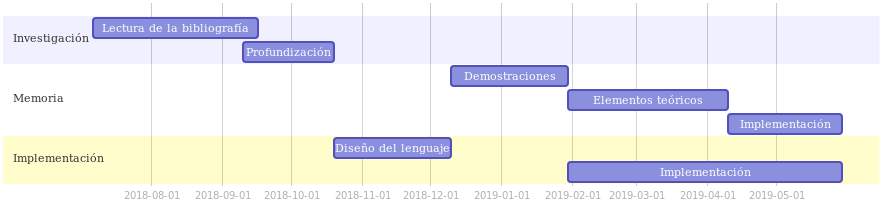
\includegraphics[width=1.6\textwidth]{imagenes/gantt1.png}
			\caption{Diagrama de Gantt del plan inicial}
			\label{fig:gantt1}
			\bigskip
			\bigskip
			\bigskip
			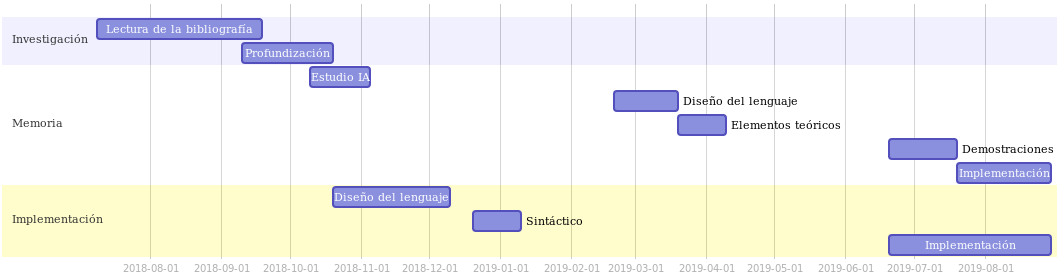
\includegraphics[width=1.6\textwidth]{imagenes/gantt2.png}
			\caption{Diagrama aproximado del trabajo real}
			\label{fig:gantt2}
		\end{center}
	\end{figure}
\end{landscape}
%
\chapter{Teoría de tipos}
\label{sect:tt}

Entre finales del siglo \rom{19} y principios del \rom{20} la teoría de conjuntos de Cantor, al mismo tiempo que experimentaba una expansión como formalismo en el que fundamentar las matemáticas, demostraba cierta inconsistencia en forma de paradojas. En 1899 el propio Cantor descubrió la primera, que se puede resumir como: Sea $T$ el cardinal del conjunto que contiene a todos los conjuntos, por como está definido, debería ser el mayor cardinal posible, sin embargo el Teorema de Cantor nos dice que $2^T > T$.\\

Sería sin embargo, en mayor media, otra paradoja la que llevaría a Russell a desarrollar los primeros elementos de la teoría de tipos, con el objetivo de eliminarla. La famosa paradoja de Russell se puede enunciar como: Sea $A = \{X : X \notin X\}$, ante la pregunta de si $A \in A$, en caso de que $A \in A$ entonces $A \notin A$ y en caso de que $A \notin A$ entonces $A \in A$. Russell haría la observación, recogida en el principio del círculo vicioso, de que estas paradojas estaban causadas por permitir expresar un conjunto por comprensión sin limitar el hecho de que se pueda hacer referencia a si mismo. Esta idea dará forma a algunos fundamentos de la teoría, como la sustitución del conjunto que contiene a todos los conjuntos por una jerarquía de ``universos".\\

Como es lógico la teoría ha sufrido un fuerte desarrollo desde la época de Russell, se ha aumentado y se han descubierto nuevos conceptos. La que nosotros estudiaremos será la llamada \textit{teoría de tipos de Martin-Löf} explicada en \textit{Homotopy Type Theory: Univalent Foundations of Mathematics} \cite{hottbook}.\\

\section{Diferencias con la teoría de conjuntos}

La principal diferencia de la teoría de tipos moderna con la teoría de conjuntos procede de la mirada particular
que se le da a su principal elemento, los tipos. No se tratan solamente como una colección que reemplaza a los conjuntos, sino que, mientras que la teoría de conjuntos tiene que construirse en el marco de un sistema deductivo como la lógica de primer orden, en la teoría de tipos los mismos tipos pueden verse como proposiciones. De esta forma demostrar una proposición representada por el tipo $A$ pasa por construir un elemento del tipo $A$.\\

Mientras que en la lógica de primer orden solo hay un tipo de sentencia, que una proposición dada tiene una demostración, la teoría de tipos cuenta con dos sentencias básicas. El análogo a ``$A$ tiene una demostración'' se escribe como ``$a : A$'' y se lee ``el término $a$ tiene tipo $A$''. Si $A$ representa una proposición se dice que $a$ es evidencia de $A$. Cuando $A$ se ve más como un conjunto que como una proposición $a:A$ es similar a $a \in A$ en la teoría de conjuntos, con una salvedad, en la teoría de conjuntos podemos considerar de forma separada el objeto $a$ sin tener en cuenta $A$, pero en la teoría de tipos todo elemento debe tener un tipo.\\

La otra sentencia disponible en la teoría de tipos es $a \equiv b : A$ o simplemente $a \equiv b$, que puede ser pensada como ``$a = b$ por definición''. En contraste, dados $a, b : A$, también se puede formar el tipo $a =_A b$, que sería el equivalente a la proposición ``$a$ y $b$ son iguales''. Si existe algún elemento del tipo $a =_A b$ decimos que $a$ y $b$ son (proposicionalmente) iguales.\\

Continuaremos presentando los tipos básicos de los que dispondremos y veremos la clara inspiración que toman de ellos los sistemas que encontramos normalmente en los lenguajes de programación.\\

\section{Tipos principales}

\subsection{Tipo función}

Dados dos tipos $A$ y $B$ podemos construir el tipo $A -> B$ de las funciones con dominio $A$ y codominio $B$. ¿Cómo? Existen dos formas, por definición directa o usando una abstracción lambda.\\

Por definición directa le damos a la función un nombre $f$ y expresamos $f : A -> B$ mediante la ecuación
$$f(x) :\equiv \Phi$$
Donde $\Phi$ es una expresión que puede involucrar a la variable $x$. Para que esta definición sea válida tenemos que demostrar que $\Phi:B$ si asumimos que $x:A$.\\

Usar una abstracción lambda nos permite no tener que dar un nombre a la función. Escribiendo la expresión $\lambda(x:A).\Phi$ tendríamos la misma definición que hemos dado con $f$. Dado que $\lambda(x:A).\Phi$ es una función podemos aplicarla a un argumento $a:A$ mediante la regla $(\lambda x.\Phi)(a) \equiv \Phi'$ donde $\Phi'$ es $\Phi$ sustituyendo todas las ocurrencias de la $x$ por $a$.\\

Para cualquier función $f:A->B$ podemos construir una función lambda $\lambda x.f(x)$ y dada la regla de aplicación podemos decir que $f \equiv (\lambda x.f(x))$. Esta igualdad nos da el principio de unicidad para los tipos función, mostrando que una función $f$ está determinada de forma única por sus valores. Esta igualdad también nos permite ver $f(x) :\equiv \Phi$ como $f :\equiv \lambda x.\Phi$.\\


\subsection{Universos y familias}

Un universo es un tipo cuyos elementos son tipos. Como se ha comentado antes si no tenemos cuidado al tratar con estos elementos podemos dar lugar a contradicciones. Para evitarlo rechazamos la existencia del universo de todos los tipos y en su lugar definimos una torre de universos $U_0:U_1:U_2:\dotsc$ donde cada $U_i$ es un elemento de $U_{i+1}$. Además si $A:U_i$ entonces también $A:U_{i+1}$. Escribiremos $A:U$ omitiendo el índice para denotar que $A$ es un tipo (i.e. reside en algún universo).\\

Llamamos familias de tipos a las funciones $B : A -> U$, que devuelven un tipo dependiendo de un parámetro $a:A$. A estas funciones también se les llama tipos dependientes y se corresponden con las familias de conjuntos en la teoría de conjuntos. Notar que dadas las restricciones sobre los universos no puede construirse una familia como $\lambda(i:\mathbb{N}).U_i$ al no existir un universo lo suficientemente grande para ser su codominio.\\


\subsection{Tipo de funciones dependientes}

Los tipos función dependientes o tipos $\Pi$ son una generalización de los tipos función. Los elementos de estos tipos son funciones cuyo codominio varía dependiendo del elemento del dominio al que son aplicadas. Dado el tipo $A:U$ y la familia $B : A -> U$, podemos construir el tipo $\Pi_{(x:A)} B(x):U$ de funciones dependientes. Cuando aplicamos una función dependiente $f:\Pi_{(x:A)} B(x)$ a un argumento $a:A$ obtenemos un elemento $f(a):B(a)$.\\

En el caso de las funciones dependientes también tenemos un principio de unicidad con $f \equiv (\lambda x.f(x))$ para todo $f:\Pi_{(x:A)} B(x)$.\\


\subsection{Tipo producto}

Dados los tipos $A,B:U$ denotamos al tipo de su producto cartesiano como $A \times B : U$. Teniendo un elemento $a:A$ y otro $b:B$ podemos construir el par $(a, b) : A \times B$. Para poder usar funciones sobre los pares introducimos una nueva regla: para cualquier $g : A -> (B -> C)$ podemos definir una función $f : A \times B -> C$ mediante $f((a, b)) :\equiv (g(a))(b)$.\\

La proyección sobre un tipo producto se define mediante las funciones:\\

\begin{align*}
  pr_1 \colon A \times B &\to A\\
  pr_1((a, b)) &:\equiv a\\
\end{align*}

\begin{align*}
  pr_2 \colon A \times B &\to B\\
  pr_2((a, b)) &:\equiv b\\
\end{align*}

Como alternativa podemos usar una función dependiente y obtener las proyecciones como casos particulares.\\

\begin{align*}
  rec_{A\times B} \colon \Pi_{C:U} (A \to B \to C) &\to A \times B \to C\\
  rec_{A\times B}(C, g, (a, b)) &:\equiv g(a)(b)\\
\end{align*}

\begin{align*}
  &pr_1 :\equiv rec_{A\times B}(A, \lambda a.\lambda b.a)\\
  &pr_2 :\equiv rec_{A\times B}(B, \lambda a.\lambda b.b)\\
\end{align*}


\subsection{Tipo de pares dependientes}
De la misma forma que el tipo de funciones dependientes generalizaba el tipo función, el tipo de pares dependientes generaliza el tipo producto permitiendo que el tipo del segundo elemento del par pueda variar en función del primer elemento. Dado el tipo $A:U$ y una familia $B : A->U$ denotamos al tipo de pares dependientes como $\sum_{(x:A)} B(x):U$. Dado un elemento $a:A$ y otro $b:B(a)$ podemos construir $(a, b) : \sum_{(x:A)} B(x):U$.\\

De la misma forma que para definir funciones sobre un tipo $A \times B$ usábamos una función auxiliar $g : A -> B -> C$, en este caso tendremos que para cualquier $g : \Pi_{(x:A)}B(x) -> C$ podemos definir una $f : (\sum_{(x:A)} B(x)) -> C$ como $f((a, b)) :\equiv g(a)(b)$.\\

Los tipos de pares dependientes se suelen utilizar para construir estructuras matemáticas. Por ejemplo, definimos un magma como un par ($A$, $m$) siendo $A:U$ un tipo y $m : A -> A -> A$ un operador binario. Dado que el tipo de $m$ depende de $A$ estamos ante un par dependiente. De esta manera podemos definir el tipo de los magmas como $Magma :\equiv \sum_{A:U} (A -> A -> A)$.\\

\subsection{Tipo de los booleanos}
Por último, y como ejemplo de un tipo más básico, introduciremos el tipo de los booleanos, escrito como $\textbf{2}:U$. Únicamente existen dos elementos con este tipo $0_2$ y $1_2$.\\

Para definir una función $f : \textbf{2} -> C$ necesitamos dos elementos $c_0, c_1:C$ para usar en las ecuaciones\\
$$f(0_2) :\equiv c_0$$
$$f(1_2) :\equiv c_1$$

También podemos definir mediante una función dependiente el equivalente a un if-then-else en un lenguaje de programación:\\

\begin{align*}
  rec_2 \colon \Pi_{C:U} C ->  C -> C &\to \textbf{2} -> C\\
  rec_2(C, c_0, c_1, 0_2) &:\equiv c_0\\
  rec_2(C, c_0, c_1, 1_2) &:\equiv c_1\\
\end{align*}


\section{De la teoría de tipos a los sistemas de tipos}
Es innegable que la teoría de tipos ha tenido gran influencia en las ciencias de la computación y en especial en el diseño de lenguajes de programación. Varios de los tipos mentados anteriormente presentan su análogo en los lenguajes más conocidos: en \textit{C} una función ``\textit{bool f(bool a, bool b);}'' estaría tipada como $f : \textbf{2} -> \textbf{2} -> \textbf{2}$ y un elemento ``\textit{'(a b)}'' de \textit{Lisp} es exactamente del tipo $A \times B$. Con respecto a las funciones y los pares dependientes han sido la inspiración para un sistema de tipos novedoso \textit{llamado sistema de tipos dependientes} que se puede encontrar en lenguajes experimentales como \textit{Idris} y que aspira a dar total libertad a la hora de elegir como de restrictivo quieres que sea el tipado de un programa.\\

Nos adentramos entonces en la parte de la teoría de tipos más aplicada, donde nos centraremos en como definir los tipos en los que estamos interesados, combinarlos en un sistema concreto, estudiar como se comporta y demostrar que tiene buenas propiedades. En este punto es fundamental el libro de Benjamin C.Pierce \textit{Types and Programming Languages} \cite{TPL}. En él se desarrolla la imagen especular de los tipos ya vistos y alguno más que nos hemos dejado en el tintero, esta vez poniendo énfasis en cómo definir su funcionamiento y de que forma introducirlos en un lenguaje.\\

%
\chapter{Sistemas de cálculo} \label{sect:sistemas_de_calculo}

Al crear un lenguaje nuestro objetivo está claro, tenemos que diseñar una herramienta que permita el cálculo de expresiones de forma más conveniente cuanto más comunes sean en nuestro contexto particular. Parece entonces sensato preguntarse qué es el cálculo, profundizar en su naturaleza y conocer sus límites. Entramos en el terreno de la Teoría de la Computación.\\
Para llevar a cabo esta tarea necesitaremos dos elementos, un modelo formal suficientemente simple que se acerque a lo que intuitivamente conocemos como cálculo y un conjunto de herramientas matemáticas que nos permitan razonar sobre este. El primero es lo que se llama un sistema de cálculo o \textit{calculi} y entre ellos el más conocido es el \textit{cálculo lambda}, el cual tomaré prestado para introducir las diferentes herramientas que usaremos a lo largo del trabajo.\\

La mejor forma de entender el funcionamiento del cálculo lambda es verlo en acción.

$$(\lambda x.x) y$$

En este pequeño ejemplo tenemos todos los componentes del cálculo lambda; el término $\lambda x.x$ se denomina abstracción lambda y es la piedra angular del sistema, a los términos $x$ e $y$ se les llama variables. Los paréntesis determinan el alcance de la abstracción, indicando que la variable $x$ se encuentra en su interior, en ese caso decimos que $x$ está ligada, mientras que $y$ sería una variable libre al no estar encerrada por ninguna abstracción.
Por último tenemos una aplicación indicada por la yuxtaposición de la abstracción $\lambda x.x$ y el término $y$, esta disposición de términos implica que se pueden sustituir todas las variables $x$ dentro de la abstracción por el término $y$, obteniendo así la evaluación $(\lambda x.x) y \to y$, que se lee como ``$(\lambda x.x) y$ evalúa a $y$".\\


Una vez conocidas todas las piezas que componen el sistema es natural preguntarnos cuáles de todas sus posibles combinaciones son válidas. Por ejemplo, ¿podemos decir que la expresión  $(\lambda x.xx) \lambda x.xz$ es válida?, para describir formalmente estas reglas tenemos que introducir nuestra primera herramienta, las gramáticas. Existen diferentes tipos de gramáticas, clasificadas por su poder expresivo, pero todas tienen el mismo objetivo, establecer de forma inequívoca qué combinaciones de términos están permitidas y proporcionar métodos sistemáticos para comprobarlo. En este trabajo utilizaré exclusivamente gramáticas libres de contexto, dado que en ningún momento habrá necesidad de mayor capacidad expresiva. Usaré para su definición la sintaxis EBNF (extended \acs{BNF}), la cual explicaré brevemente a continuación al mismo tiempo que introduzco la gramática del cálculo lambda.\\

\begin{grammar}{t}{términos}
x             & variable \\
\lambda x.t     & abstracción \\
t\ t           & aplicación
\end{grammar}

\begin{grammar}{v}{valores}
\lambda x.t     & valor abstracción
\end{grammar}

\bigskip

Lo que esta notación nos dice es que a los términos del cálculo lambda les damos la etiqueta $t$, y un término puede ser una variable, una abstracción o una aplicación.
A su vez a los valores les damos la etiqueta $v$ y solamente las abstracciones son consideradas como valores.
La utilidad de distinguir entre términos y valores la veremos a continuación, pero de forma general podemos decir que los valores serán los únicos resultados posibles
tras finalizar la evaluación de una expresión.
Las abstracciones se codifican como ``$\lambda x.$''` junto con un término y las aplicaciones situando un término al lado de otro. De esta forma vemos que, efectivamente, $(\lambda x.xx) \lambda x.xz$ es una expresión válida, ya que las abstracciones son términos y una aplicación se puede producir entre dos términos cualesquiera. Pero aún nos queda una pregunta, ¿cómo se evalúa esta expresión? De la misma forma que podemos formalizar la sintaxis y la gramática del sistema podemos formalizar su significado, es decir, su semántica.\\

A la hora de especificar una semántica existen varios tipos de formalismos, nosotros usaremos la llamada semántica operacional (operational semantics), especialmente conveniente para lenguajes funcionales (i.e. aquellos fundamentados sobre el cálculo lambda). Es esta herramienta la que nos muestra el significado concreto de ``computar'' aplicado al cálculo lambda, que no es otra cosa que reescribir una expresión sustituyendo la variable ligada de una abstracción por el término situado a su izquierda.\\

\[
\inference[E-Aplicación1:]{t_1 -> t_1'}{t_1\ t_2 -> t_1'\ t_2}\\
\]
\[
\inference[E-Aplicación2:]{t_2 -> t_2'}{v_1\ t_2 -> v_1\ t_2'}\\
\]
\[
\inference[E-Sustitución:]{}{(\lambda x.t_{12})v_2 -> [x |-> v_2]t_{12}}
\]
\bigskip

La semántica operacional se compone de reglas, llamadas reglas de evaluación, las cuales toman prestada la notación de la deducción natural, donde si se cumple la proposición superior de la regla podemos deducir que también se cumple la inferior. Por ejemplo la regla (E-Aplicación1) se leería como ``si el término $t_1$ puede evaluarse a $t_1'$ entonces la expresión $t_1\ t_2$ puede evaluarse a $t_1'\ t_2$''. Notar que la regla (E-Aplicación2) es también la condición de parada de (E-Aplicación1) y entre las dos definen un orden de evaluación: primero se evalúa el término de la izquierda hasta obtener un valor y a continuación se evalúa el de la derecha.
Por último la notación utilizada en (E-Sustitución) $[x |-> v_2]t_{12}$ es equivalente al término $t_{12}$ sustituyendo todas las ocurrencias de $x$ por $v_2$, es decir $[x |-> v]xyx$ equivaldría a $vyv$.\\

Establecidas estas reglas ya podemos evaluar cualquier expresión. Veamos por ejemplo cual es el valor de $(\lambda x.x) (\lambda y.y) ((\lambda x.x) (\lambda z.(\lambda x.x) z))$:\\


\begin{gather*}
\inference[E-Sustitución:]{}{(\lambda x.x)(\lambda y.y) -> (\lambda y.y)} \\
\inference[E-Aplicación1:]{}{
\begin{array}{@{}c@{}}
(\lambda x.x) (\lambda y.y) ((\lambda x.x) (\lambda z.(\lambda x.x) z)) -> \\
 -> (\lambda y.y) ((\lambda x.x) (\lambda z.(\lambda x.x) z))
\end{array}} \\
\inference[E-Sustitución:]{}{(\lambda x.x) (\lambda z.(\lambda x.x) z) -> \lambda z.(\lambda x.x) z} \\
\inference[E-Aplicación2:]{}{
\begin{array}{@{}c@{}}
(\lambda y.y) ((\lambda x.x) (\lambda z.(\lambda x.x) z)) -> \\
 -> (\lambda y.y) (\lambda z.(\lambda x.x) z)
\end{array}} \\
\inference[E-Sustitución:]{}{(\lambda y.y) (\lambda z.(\lambda x.x) z) -> \lambda z.(\lambda x.x) z}
\end{gather*}
\bigskip


Tenemos así que $(\lambda x.x) (\lambda y.y) ((\lambda x.x) (\lambda z.(\lambda x.x) z)) ->^{*} \lambda z.(\lambda x.x) z$, donde $->^{*}$ significa que una expresión evalúa a otra en varios pasos. Como vemos, la notación utilizada nos permite tratar la salida de una regla como la entrada de otra, pudiendo escribir razonamientos de forma compacta y cómoda.\\

Con lo presentado hasta ahora podemos describir de manera inequívoca un lenguaje simple como el calculo lambda, pero si queremos añadir restricciones más complejas para obtener ciertas propiedades necesitamos echar mano de los sistemas de tipos.\\


\section{Restricción del lenguaje mediante sistemas de tipos}

Hasta ahora hemos usado el cálculo lambda como excusa para introducir las herramientas
necesarias para describir con precisión su sintaxis y sus reglas de evaluación.
Para hacer lo mismo con las reglas de tipado necesitaremos extender el sistema para
que acepte tipos, es decir, necesitamos un nuevo lenguaje, el llamado calculo lambda
simplemente tipado (simply typed lambda calculus).\\

Como ya hemos visto, lo primero a la hora de representar un lenguaje es definir su sintaxis.
La sintaxis del cálculo lambda simplemente tipado es similar a la del cálculo lambda ordinario, la única 
diferencia es que se añade nueva notación para indicar qué tipos aceptan las abstracciones. Estas diferencias
se encuentran marcadas en rojo en la siguiente gramática:\\

\begin{grammar}{t}{términos}
  x             & variable \\
  \lambda x\textcolor{myred}{:T}.t     & abstracción \\
  t\ t           & aplicación
\end{grammar}

\begin{grammar}{v}{valores}
  \lambda x\textcolor{myred}{:T}.t     & valor abstracción
\end{grammar}

{\color{myred}
\begin{grammar}{T}{tipos}
  T \to T    & tipo función
\end{grammar}
}

{\color{myred}
\begin{grammar}{\Gamma}{contexto}
  \o    & contexto vacío \\
  \Gamma,x:T    & asociación entre tipo y variable
\end{grammar}}

\bigskip

Lo primero que destaca es la notación ``$:T$'', la cual indica que una abstracción solo acepta parámetros del tipo $T$. Un tipo $T$ se construye mediante la sintaxis $T_1 \to T_2$, que es el tipo definitorio de una
función cuyo dominio son elementos del tipo $T_1$ y su imagen son elementos del tipo $T_2$.\\

Por último se define la representación de lo que llamamos un contexto. Para poder comprobar que una aplicación
tiene el tipo correcto (que el tipo de la expresión que pasamos a la abstracción coincide con el tipo de la abstracción) necesitamos conocer el tipo de todas las expresiones y por tanto tenemos que tratar el tipo asignado a cada expresión como una propiedad global del sistema (algo a lo que podemos acceder en cualquier momento), ahí es donde entra nuestro contexto. El contexto $\Gamma$ es simplemente una lista en la que se guarda el tipo que se le ha asignado a cada expresión, y usaremos la notación $\Gamma |- x:T$ para decir ``del contexto $\Gamma$ se deduce que $x$ tiene el tipo $T$''. Por ejemplo si $\Gamma = \o, x_1:T_1, x_2:T_2$ entonces $\Gamma |- x_1:T_1$.\\

Sobre las reglas de evaluación del cálculo lambda simplemente tipado no hay mucho que decir, son las mismas que
teníamos en el cálculo lambda con las adiciones sintácticas que hemos visto.\\

\[
\inference[E-Aplicación1:]{t_1 -> t_1'}{t_1\ t_2 -> t_1'\ t_2}\\
\]
\[
\inference[E-Aplicación2:]{t_2 -> t_2'}{v_1\ t_2 -> v_1\ t_2'}\\
\]
\[
\inference[E-Sustitución:]{}{(\lambda x\textcolor{myred}{:T_{11}}.t_{12})v_2 -> [x |-> v_2]t_{12}}
\]
\bigskip

Así llegamos al que es el propósito de esta sección, la nueva herramienta que nos permitirá definir nuestro sistema de tipos, las reglas de tipado. Estas reglas funcionan con la misma lógica que la semántica operacional, la diferencia es que en vez de hablar sobre la forma en que las expresiones se evalúan habla de cómo el tipo de una
expresión es deducido, y dado que solamente las expresiones que puedan ser producidas a través de estas reglas
son válidas en nuestro lenguaje, también impone restricciones sobre que combinaciones de tipos son válidas y cuales no.

\[\inference[T-Var:]{x:T \in \Gamma}{\Gamma |- x:T}\]

\[\inference[T-Abs:]
  {\Gamma,x:T_1 |- t_2:T_2}
  {\Gamma |- \lambda x:T_1.t2\ :\ T_1 -> T_2}
\]

\[\inference[T-Ap:]
  {\Gamma |- t_1:T_{11}->T_{12}\ \ \Gamma |- t_2:T_{11}}
  {\Gamma |- t_1\ t_2:T_{12}}
\]

La premisa de (T-Var), $x:T \in \Gamma$, se lee como ``El tipo asumido para x en $\Gamma$ es $T$''. Esto, como veremos, nos proporciona una regla para construir un contexto desde el que se pueda deducir que $x:T$. La regla (T-Abs) nos dice que, si en nuestro contexto tenemos que la variable de la abstracción está asociada al tipo $T_1$ y se deduce que el cuerpo de la abstracción tiene el tipo $T_2$, a esta abstracción le corresponderá el tipo de una función que lleva elementos del tipo $T_1$ en elementos del tipo $T_2$. Por último la regla (T-Ap) impone la restricción de que en las aplicaciones la expresión de la izquierda debe ser un tipo función y la de la derecha tiene que tener el mismo tipo que su dominio.\\

Para ver el funcionamiento de este sistema demostraremos que $(\lambda x:Bool.x)true$ tiene como tipo $Bool$. En este caso consideraremos que $Bool$ es un tipo primitivo y añadiremos la regla \inference[T-True:]{}{\o |- true:Bool}.\\

\[\inference[T-Ap:]
  {\inference[T-Abs:]
    {\inference[T-Var:]
      {x:Bool \in x:Bool}
      {x:Bool |- x:Bool}}
    {\o |- \lambda x:Bool.x : Bool -> Bool}
   \quad
   \inference[T-True:]{}
    {\o |- true:Bool}}
  {\o |- (\lambda x:Bool.x)true : Bool}
\]

\bigskip

Dado que la regla (T-Ap) construye un contexto donde la combinación de tipos es válida y debido a la regla (T-Abs), solo tiene sentido que en el contexto aparezca $x:T$ si existe la etiqueta $\lambda x:T$, así desde un punto de vista práctico podemos leer $x:T \in \Gamma$ como ``La etiqueta x:T se encuentra en la expresión''.\\

Notar que en base a este sistema de tipos, una expresión como $(\lambda x:Int.x)true$ sería rechazada, ya que
no existe ninguna derivación mediante la que pueda tiparse. De esta forma ganamos control sobre que clase de
parámetros pueden o no recibir las abstracciones. Sin embargo, añadir un sistema de tipos a un lenguaje
puede tener ventajas que van incluso más allá de mejorar el control que se tiene sobre él, se puede forzar
a que el lenguaje cumpla ciertas propiedades y el cálculo lambda simplemente tipado es un gran ejemplo de esto.\\

\begin{theorem}[Normalization property]
  La evaluación de un programa bien tipado en el cálculo lambda simplemente tipado termina en un número finito de pasos.
\end{theorem}

Ya que la demostración de este teorema requiere de técnicas de normalización que no son relevantes para el resto del trabajo y se puede encontrar en \cite{TPL}, no se abordará. En todo caso, la observación fundamental es
que, simplemente añadiendo un sistema de tipos, hemos sido capaces de asegurar algo tan deseable como 
que cualquier programa escrito en este lenguaje siempre termina. Evidentemente esta propiedad no podía venir sin
un coste, y es que, debido al problema de la parada, el cálculo lambda simplemente tipado no puede ser turing-completo.\\

A pesar de todo, este ejemplo nos sirve como incentivo para estudiar qué otras propiedades podrían ser deseables
en un lenguaje de programación. A la que nosotros prestaremos más atención será a si nuestro lenguaje es seguro.\\

\begin{definition}[Forma normal]
  Un término $t$ está en forma normal si no se le puede aplicar ninguna regla de evaluación (i.e no existe $t'$ tal que $t -> t'$).
\end{definition}

\begin{definition}[Término atascado]
  Decimos que un término cerrado (término sin variables libres) se encuentra atascado (in stuck state) si está
  en forma normal pero no es un valor.
\end{definition}

\begin{definition}[Seguridad]
  Decimos que un sistema de tipos es seguro (safe o sound) si cualquier término bien tipado no se queda atascado.
  Diremos también que un lenguaje es seguro si su sistema de tipos lo es.
\end{definition}


Es evidente que poder garantizar la seguridad de un lenguaje es extremadamente útil en la práctica ya que el
programa o bien seguirá ejecutándose o eventualmente llegará a un valor final. Evitamos así situaciones en
las que su comportamiento no está determinado, como por ejemplo leer en una posición de memoria no reservada en \textit{C}.\\

Esta propiedad es tan importante en la Teoría de Lenguajes de Programación que se ha desarrollado un procedimiento estándar para demostrarla en un lenguaje arbitrario. Esta demostración se realiza en dos pasos a
través de los teoremas de \textit{progreso} y \textit{preservación}.

\begin{theorem}[Progreso]
  Un término bien tipado no está atascado.
\end{theorem}

\begin{theorem}[Preservación]
  Si un término está bien tipado, tras un paso de evaluación lo sigue estando.
\end{theorem}

Si podemos demostrar que un determinado lenguaje cumple ambas propiedades habremos deducido con éxito que un término bien tipado nunca puede quedarse atascado durante su evaluación. Como ejemplo y para terminar esta sección, veamos como podríamos demostrar que el cálculo lambda simplemente tipado es seguro. Esta demostración está extraída directamente del capítulo 9 de \textit{Types and Programming Languages} \cite{TPL}.\\

\begin{theorem}[Progreso del cálculo lambda simplemente tipado]
\label{theo:prog_lambda}
  Sea $t$ un término cerrado y bien tipado (i.e. $\o |- t:T$ para algún $T$), entonces o bien $t$ es un valor o existe algún $t'$ tal que $t -> t'$.
\end{theorem}

\begin{proof}
  La demostración se realizará por inducción sobre las posibles derivaciones de $t$. Para ello es necesario introducir el concepto de subtérmino. Si $t$ es un término en el que a su vez aparecen los términos $t_1, t_2, ..., t_n$ diremos que estos son subtérminos inmediatos de $t$. Por ejemplo $x$ sería un subtérmino inmediato de $\lambda x.x$.\\
  
  Así, supuesto cierto el progreso para todos los subtérminos inmediatos de $t$ podemos poner en marcha la inducción.\\
  
  Según nuestra gramática tenemos tres casos posibles:
  \begin{enumerate}
    \item Que $t$ sea una variable ($t = x$).
    \item Que $t$ sea una abstracción ($t = \lambda x:T.t'$).
    \item Que $t$ sea una aplicación ($t = t_1\ t_2$).
  \end{enumerate}
  
  El primer caso no se puede dar ya que $t$ es un término cerrado y no hay ninguna regla que permita que durante
  la evaluación un término cerrado deje de serlo.\\
  
  El segundo caso es trivial, ya que una abstracción es un valor.\\
  
  El tercer caso es el más interesante. Por hipótesis de inducción $t_1$ o bien será un valor o podrá evaluarse un paso más. Lo mismo pasa con $t_2$. Además al ser $t$ un término bien tipado necesariamente $\o |- t1:T_{11} -> T_{12}$ y $\o |- t2:T_{11}$. Tenemos así tres casos posibles:\\
  
  \begin{itemize}
    \item Si existe un $t'_1$ tal que $t_1 -> t'_1$ entonces aplicando la regla (E-Aplicación1) $t -> t'_1\ t_2$.
    
    \item Si $t_1$ es un valor y $t_2 -> t'_2$ aplicando (E-Aplicación2) tenemos que $t -> t_1\ t'_2$.
    
    \item Si $t_1$ y $t_2$ son valores. Como $t1:T_{11} -> T_{12}$, $t_1$ tendrá la forma $\lambda x:T_{11}.t_{12}$, por lo que aplicando (E-Sustitución) obtendremos $t -> [x -> t_2]t_1$.
  \end{itemize}
  
\end{proof}


\begin{theorem}[Preservación del cálculo lambda simplemente tipado]
\label{theo:pres_lambda}
  Sea $t$ un término cerrado y bien tipado con $\Gamma |- t:T$ y $t -> t'$ entonces $\Gamma |- t':T$.
\end{theorem}

\begin{proof}
  Aplicaremos inducción sobre las subderivaciones, sinedo la hipótesis que si $s:S$ y $s -> s'$ entonces $s':S$. Veamos caso por caso con que regla podríamos deducir que $t:T$.\\
  
  \begin{itemize}
    \item \textbf{(T-Var):} En este caso deducimos que $t=x$ y $x:T$.\\
    Dado que $t$ es un término no cerrado no tenemos en cuenta este caso.\\
    
    \item \textbf{(T-Abs):} En este caso deducimos que $x:T_1$, $t_2:T_2$ y $t=\lambda x:T_1.t_2$.\\
    En este caso $t$ es un valor y se cumplen las condiciones del teorema por omisión.
    
    \item \textbf{(T-Ap):} En este caso deducimos que $t_1:T_{11} -> T_{12}$, $t_2:T_{11}$ y $t = t_1t_2$.\\
    Con este $t$ hay tres reglas que permiten la evaluación $t -> t'$:\\
    
    \begin{itemize}
      \item \textbf{(E-Aplicación1):} Deducimos que $t_1 -> t'_1$ y por hipótesis de inducción $t'_1:T_{11} -> T_{12}$. Entonces $t -> t' = t'_1t_2$ y aplicando (T-Ap) tenemos que $t':T_{12}$.\\
      
      \item \textbf{(E-Aplicación2):} Deducimos que $t_1 = v_1$ es un valor y $t_2 -> t'_2$. Por hipótesis de inducción $t'_2:T_{11}$. Entonces $t -> t' = v_1t'_2$ y aplicando (T-Ap) tenemos que $t':T_{12}$.\\
      
      \item \textbf{(E-Sustitución):} Deducimos que $t_1 = \lambda x:T_{11}.t_{12}$ y que $t_2 = v_2$ es un valor. Como $t_1:T_{11} -> T_{12}$, dado un valor $v:T_{11}$ necesariamente $[x |-> v]t_{12} : T_{12}$. Entonces $t -> t' = [x |-> v_2]t_{12}$ y tenemos que $t':T_{12}$.\\
    \end{itemize}
  \end{itemize}
\end{proof}

%
\chapter{Aplicación a la inteligencia artificial}
\label{sect:ap_ia}

Uno de los problemas más frustrantes encontrado a la hora de trabajar en algún proyecto que presente un mayor enfoque en los algoritmos, especialmente aquellos que involucran alguna forma de inteligencia artificial, es que el lenguaje en el que se trabaja parece interponerse en tu camino.
Cuando se diseña un sistema complejo desde el punto de vista de arquitectura de software los objetos y las clases te proporcionan una ayuda invaluable para su organización, si estas diseñando una web tienes lenguajes específicos que te ayudan a estructurar su estética, incluso cuando programas a bajo nivel dispones de herramientas que te proporcionan un control total sobre la máquina y, si es posible, te ayudan a no cometer errores.\\

Sin embargo parece que al trabajar con \acs{IA} debemos escoger el lenguaje menos malo. \textit{Python} parece un buen candidato y en efecto muchos lo usan, es agradable y no se mete mucho en tu camino, sin embargo esto es a costa de un buen rendimiento y de la corrección que proporciona un sistema de tipos. Con \textit{Java} tienes esto último, pero introduciendo una cantidad de papeleo inmensa para hacer lo más básico, lo cual no es muy agradable si lo único que quieres es centrarte en los algoritmos. Por último, si necesitas velocidad podrías decidirte por \textit{C++}, en este caso te dará más problemas el manejo de memoria que la lógica del propio programa.
No hemos puesto estos lenguajes como ejemplo de forma arbitraria, sino que son, como veremos a continuación, algunos de los más usados en IA.\\


En esta capítulo recopilaremos las características que harían de un lenguaje una herramienta óptima para codificar los problemas a los que se enfrenta la inteligencia artificial. Seguramente la solución que obtengamos no sea ni mucho menos la óptima, tampoco se pretende, nos conformamos con poder aportar alguna idea interesante.\\


\section{Justificación para un lenguaje orientado a la IA}
¿Por qué diseñar un lenguaje especifico para inteligencia artificial? ¿Se gana algo frente a los lenguajes ya existentes?

Uno de los argumentos más contundentes en contra de un lenguaje para IA es que, de hecho, no puede existir, el campo es muy poco definido, utiliza muchas técnicas diferentes y evoluciona demasiado rápido. La mejor aproximación no pasaría por crear un lenguaje específico sino por implementar librerías de calidad para cada caso.
Nuestra respuesta es que esto no explica el porqué algunos lenguajes son más usados que otros en IA y las librerías especializadas parecen acumularse en estos mientras que otros carecen de ellas. Pareciera que hay elementos que hacen de algunos entornos especialmente atractivos para la implementación de algoritmos de inteligencia artificial. \\

Desafortunadamente no hemos encontrado ningún estudio al respecto, así que se ha realizado un pequeño análisis utilizando datos de GitHub. Primero vamos a ver en que lenguajes están escritos los 500 repositorios más populares (con más estrellas) que aparecen en GitHub al buscar ``artificial intelligence'':\\

\begin{lstlisting}[style=python, caption={Script para obtener el número de proyectos por lenguaje entre los 500 proyectos más importantes de Github}]
import itertools
import time
from github import Github
import matplotlib.pyplot as plt
import matplotlib.ticker as ticker


# Devuelve un diccionario que asocia a cada lenguaje su número de repositorios
def count_repos_by_lang(repos):
	repos_by_lang = {}

	for repo in repos:
		lang = repo.language
		if lang is None:
			continue
		# Si el lenguaje principal es Jupyter Notebook utilizamos el segundo más usado
		if lang == 'Jupyter Notebook':  
			languages = repo.get_languages()
			# En caso de que el único lenguaje sea Jupyter Notebook
			if len(languages) == 1:
				continue
			lang = sorted(languages, key=languages.get, reverse=True)[1]
		repos_by_lang[lang] = repos_by_lang.get(lang, 0) + 1

	return repos_by_lang


# Iniciamos sesión en GitHub
g = Github("usuario", "clave")

# Obtenemos los 500 repositorios más populares en inteligencia artificial
ai_repos = itertools.islice(g.search_repositories("artificial intelligence", sort="stars"), 500)
ai_repos_by_lang = count_repos_by_lang(ai_repos)

# Los disponemos en una gráfica
plt.bar(list(ai_repos_by_lang.keys()), list(ai_repos_by_lang.values()), color=(0.16, 0.5, 0.73, 1))
plt.xticks(rotation=90, fontsize='8')
plt.yticks(fontsize='8')
plt.subplots_adjust(bottom=0.2)
plt.show()
\end{lstlisting}

Los resultados obtenidos se presentan en la figura \ref{fig:ailang}.\\

\begin{figure}[h]
  \begin{center}
    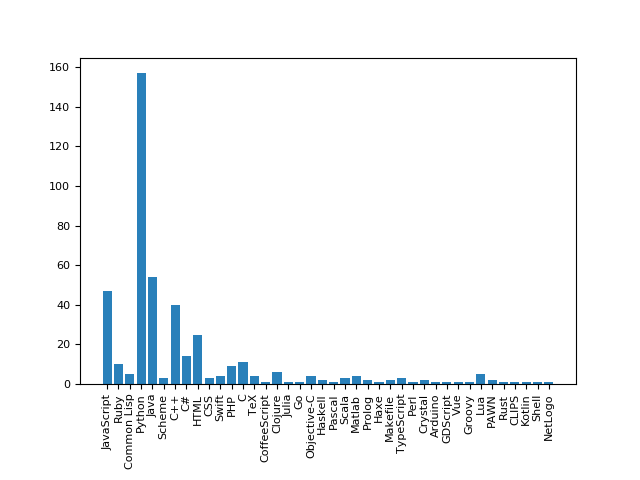
\includegraphics[width=1.0\textwidth]{imagenes/ai-lang.png}
    \caption{Número de proyectos por lenguaje entre los 500 proyectos de IA más populares de Github}
    \label{fig:ailang}
  \end{center}
\end{figure}

A priori parece que es cierto que hay lenguajes que destacan más en el campo de la inteligencia artificial, pero cabe la posibilidad de que estos datos simplemente reflejen la popularidad de cada lenguaje. Para descartar esto obtendremos los 500 repositorios más populares de GitHub y calcularemos el ratio de uso en IA frente al uso general de cada lenguaje:\\

\begin{lstlisting}[style=python, caption={Script para obtener el ratio entre proyectos de IA y proyectos generales por lenguaje en Github}]
# Obtenemos los 500 repositorios más populares de GitHub
popular_repos = itertools.islice(g.search_repositories("stars:>1", sort="stars"), 500)
popular_repos_by_lang = count_repos_by_lang(popular_repos)

# Calculamos el ratio de uso de cada lenguaje en proyectos de ia y en general
proportion_by_lang = {}
for lang in ai_repos_by_lang.keys():
	proportion_by_lang[lang] = ai_repos_by_lang[lang] / popular_repos_by_lang.get(lang, -1)

# Lo disponemos en una gráfica
plt.axes().yaxis.set_minor_locator(ticker.MultipleLocator(1))
plt.axhline(y=0, linewidth=0.75, color=(0.27, 0.27, 0.27))
plt.axhline(y=1, linewidth=0.35, color=(0.27, 0.27, 0.27))
plt.bar(list(proportion_by_lang.keys()), list(proportion_by_lang.values()), color=(0.16, 0.5, 0.73, 1))
plt.xticks(rotation=90, fontsize='8')
plt.yticks(fontsize='8')
plt.subplots_adjust(bottom=0.2)
plt.show()
\end{lstlisting}

Notar que si un lenguaje se ha usado en proyectos de IA pero no en proyectos generales el ratio sería infinito, en este caso le asignaremos como valor el número de repositorios de IA en el que se usa pero en negativo, para que no haya confusión. Teniendo esto en cuenta los resultados quedan como se muestra en la figura \ref{fig:proplang}.\\

\begin{figure}[h]
  \begin{center}
    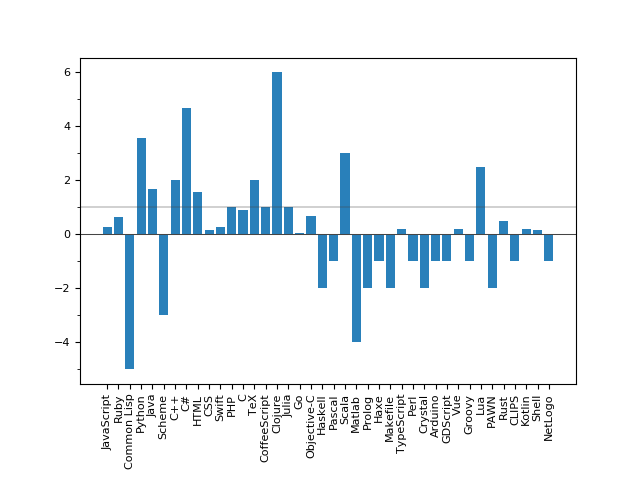
\includegraphics[width=1.0\textwidth]{imagenes/proportion-lang.png}
    \caption{Ratio entre proyectos de IA y proyectos generales por lenguaje en Github.}
    \label{fig:proplang}
  \end{center}
\end{figure}

Los lenguajes con un ratio menor que 1 son menos usados en IA que en otro tipo de proyectos y viceversa. Esto claramente no es un estudio serio, contiene bastantes errores que pueden arrojar datos imprecisos, por ejemplo depende de lo que GitHub entienda como ``artificial intelligence'' en su búsqueda. Además los ratios de algunos lenguajes pueden explicarse por sus particularidades, por ejemplo HTML y CSS, siendo lenguajes específicos del diseño web, es esperable que no puntúen muy bien. Sin embargo creo que cumple con la intención de señalar que realmente hay lenguajes que atraen a los desarrolladores de IA más que otros. Entonces cabe preguntarse ¿por qué? Estas diferencias pueden deberse a múltiples factores: librerías, comunidad, soporte de herramientas (p.e. debuggers, gestores de paquetes), tradición, etc. Sin embargo estos elementos tienen que formarse alrededor de un lenguaje, por lo tanto este tiene que ofrecer un potencial que otros no, pero además esto nos lleva a otro punto a favor de un lenguaje especializado en IA.\\

Que un lenguaje esté especializado en inteligencia artificial no solo significa que adapte su sintaxis o que tenga determinados constructos semánticos especialmente útiles (lo cual no es poca cosa), significa que gran parte del esfuerzo estará dirigido a tener un entorno lo más adaptado posible. Significa que se podrán invertir recursos en tener las mejores librerías de NPL, ML, planificación, estadística, etc posibles. Que las herramientas tales como debuggers estarán pensadas especialmente para resolver los problemas que plantee este campo sin dividir recursos en las necesidades que puedan surgir de, por ejemplo, la programación web o la de sistemas. También quiere decir que todas estas herramientas y librerías podrían estar al día de los últimos avances en investigación. En definitiva, una menor superficie nos permite enfocar mejor nuestros esfuerzos.\\


\section{Cómo diseñar un lenguaje orientado a la IA}
Que un lenguaje para IA tenga sentido no quiere decir que las objeciones planteadas arriba estén erradas, ciertamente el hecho de que la inteligencia artificial como campo esté muy pobremente definido y que se mueva muy rápido plantea muchas dificultades.\\

Por estas razones no es factible que este lenguaje sea un \acs{DSL}, como podría serlo uno orientado a un dominio más concreto (p.e. \textit{Prolog} en programación lógica), sino que deberá ser un lenguaje de propósito general, pero con ciertas características especialmente convenientes.
El ejemplo más próximo sería trasladar lo que ha hecho \textit{Julia} en el área de la computación numérica a la inteligencia artificial.
Para extraer estas características primero debemos conocer las necesidades más habituales a la hora de implementar una IA.\\

\subsection{Peculiaridades de la inteligencia artificial como ingeniería de software}
Günter Neumann en \cite{neumann_programming_nodate} rescata ciertos elementos que diferencian el trabajo en inteligencia artificial del de otras áreas y que explicarían porqué \textit{Lisp} y \textit{Prolog} han sido lenguajes tan relevantes en este campo:\\

\begin{itemize}
  \item La IA se centra en la computación simbólica más que en el procesamiento de números, siendo especialmente adecuados para el manejo de símbolos los lenguajes declarativos.\\
  
  \item La especificación inicial de un problema de IA es compleja, es más eficaz desarrollar los algoritmos de forma gradual mediante prototipos.\\
  
  \item Los algoritmos de IA no requieren de un control total de la máquina, por lo que es beneficioso un mayor nivel de abstracción que libere al programador de detalles de bajo nivel como el manejo de memoria.\\
\end{itemize}

Aunque algunos de estos puntos ya han sido superados y los vemos como normales en los lenguajes actuales (incluso se podría discutir el primero dada la importancia de la estadística en la IA moderna), hay que tener en cuenta que antes de que \textit{Lisp} introdujese avances como la recolección de basura lo mejor que se tenía era \textit{Fortran}, que se especializaba en el puro procesamiento numérico.\\

Nos permitiremos añadir otros factores que, con base en la teoría computacional de la mente explicada de forma muy accesible por Steven Pinker en \textit{How the Mind Works} \cite{how_mind_works} y por experiencia personal, en nuestra opinión también caracterizan al campo:\\

\begin{itemize}
  \item Mayor énfasis en los algoritmos que en el diseño de software.
  
  \item Ejecuciones largas, se necesita algún mecanismo que asegure que el programa no va a fallar después de varias horas de ejecución por escribir mal el nombre de una variable.
  
  \item Consumo de recursos considerable.
  
  \item Uso de herramientas lógicas y estadísticas, siendo particularmente útil la capacidad de codificar objetivos y modelos del mundo.
  
  \item Frecuente manejo de diferentes estructuras de datos.
  
  \item Concurrencia. Muchos de nuestros procesos mentales ocurren en paralelo.
  
  \item Necesidad de feedback continuo. Esto ayuda en el proceso de ensayo y error que supone calibrar un algoritmo.
  
  \item Visualización y comparación de resultados.
  
  \item Diseño modular que facilite la integración de distintas herramientas de forma organizada.
\end{itemize}


Creemos que un lenguaje que de respuesta a estas particularidades es un buen candidato para ser usado en IA más allá de las diferentes modas que puedan sucederse.


\section{Aspectos principales de nuestro lenguaje}
Intentemos esbozar los principales componentes de un lenguaje pensando en dar solución a los puntos anteriores.

Parece buena idea establecer una lista de prioridades en características que puedan estar en conflicto. Esto permite simplificar la elección de introducir o no un elemento que requiere un ``trade-off'' entre alguna de estas. Basta ver si la característica que se beneficia tiene más prioridad que la que sale perjudicada. Para este caso la siguiente lista me parece razonable:

\begin{enumerate}
  \item Velocidad de implementación, testeo y cambio.
  
  \item Eficiencia.
  
  \item Corrección de los programas.
\end{enumerate}


\subsection{Runtime}
\subsubsection*{Sistema de traducción: Compilado AOT vs Interpretado vs JIT}
Veamos las ventajas e inconvenientes de cada uno de los tipos.\\

\textbf{Compilación AOT:}\\

\begin{itemize}
  \item {\color{okgreen} Ventaja}: Produce código muy eficiente.\\
  \item {\color{okgreen} Ventaja}: Solo pasa por el proceso de traducción una vez.\\
  \item {\color{okgreen} Ventaja}: Quien recibe el ejecutable no necesita tener un compilador instalado.\\
  \item {\color{myred} Inconveniente}: Cada vez que se quiera probar un cambio hay que volver a compilar. Puede paliarse con un buen sistema de compilación.\\
\end{itemize}

\textbf{Interpretación:}\\

\begin{itemize}
  \item {\color{okgreen} Ventaja}: Mayor flexibilidad (p.e. pueden modificarse a si mismos en tiempo de ejecución).\\
  \item {\color{okgreen} Ventaja}: No hay que compilar cada cambio.\\
  \item {\color{myred} Inconveniente}: Tiene más limitaciones a la hora de hacer eficiente el código.\\
  \item {\color{myred} Inconveniente}: Pasa por el proceso de traducción cada vez que se ejecuta el programa.\\
\end{itemize}

\textbf{Compilación JIT:}\\

\begin{itemize}
  \item {\color{okgreen} Ventaja}: Mantiene todas las ventajas de la interpretación.\\
  \item {\color{okgreen} Ventaja}: La eficiencia es cercana a la de la compilación AOT, incluso en algunos casos puede hacer optimizaciones específicas con los datos de la ejecución actual y los del entorno donde se ejecuta.\\
  \item {\color{myred} Inconveniente}: La compilación se realiza en cada ejecución.\\
  \item {\color{myred} Inconveniente}: Algunas optimizaciones que realizaría un compilador AOT son demasiado costosas para ser hechas en tiempo de ejecución.\\
  \item {\color{myred} Inconveniente}: Es complicado de implementar comparado con la interpretación y la compilación AOT. 
\end{itemize}

En nuestra opinión, el sistema que mejor cumple nuestros requisitos sería un compilador JIT con opción de compilación AOT. De esta forma conseguimos un workflow ágil con bastante eficiencia y en caso de que el overhead del JIT no sea aceptable o se necesite un ejecutable independiente se podría compilar AOT.
La principal desventaja sería la dificultad de implementación, que ya de por sí es elevada con un solo traductor (sobre todo en el caso de un JIT).


\subsubsection*{Manejo de memoria: manual vs GC vs ownership}

\textbf{Manual:}\\

\begin{itemize}
  \item {\color{okgreen} Ventaja}: Control total sobre la memoria, lo que permite programas más eficientes. \\
  \item {\color{myred} Inconveniente}: El programador debe razonar sobre la memoria, lo cual consume ``espacio cognitivo'' para pensar en los algoritmos.\\
  \item {\color{myred} Inconveniente}: Es un sistema propenso a fallos que además no pueden detectarse en tiempo de compilación (El lenguaje no es seguro).\\
\end{itemize}

\textbf{Recolector de basura:}

\begin{itemize}
  \item {\color{okgreen} Ventaja}: El programador se despreocupa del manejo de la memoria.\\
  \item {\color{okgreen} Ventaja}: Permite lenguajes seguros.\\
  \item {\color{myred} Inconveniente}: Añade overhead a la ejecución.\\
  \item {\color{myred} Inconveniente}: Aumenta la complejidad del compilador.\\
\end{itemize}

\textbf{Ownership (à la \textit{Rust}):}

\begin{itemize}
  \item {\color{okgreen} Ventaja}: Permite lenguajes seguros, los fallos de memoria se detectan en tiempo de compilación.\\
  \item {\color{okgreen} Ventaja}: No añade overhead.\\
  \item {\color{myred} Inconveniente}: El programador sigue teniendo que razonar sobre la memoria, además con restricciones sobre su uso.\\
\end{itemize}

Dado que tanto el manejo manual como el ownership distraen al programador de su tarea principal y dificultan el realizar cambios en el código, siguiendo nuestra lista de prioridades la única opción factible que nos queda es usar un recolector de basura.\\


\subsection{Sistema de tipos}
La primera elección que tenemos que tomar claramente es si queremos un sistema de tipos, es decir, si nuestro lenguaje va a ser débilmente o fuertemente tipado.\\

Un sistema débil proporciona más flexibilidad y rapidez en la implementación, pero uno fuerte da herramientas para asegurar cierto buen comportamiento de los programas y la información extra puede aprovecharse para generar código más eficiente.\\

Por suerte existe una forma de obtener las ventajas de ambos sistemas, el tipado gradual. Un lenguaje con este sistema permitiría prototipados que pueden cambiarse rápidamente y una vez que se ha llegado a una versión definitiva poder garantizar cierta corrección. Me parece el sistema ideal a la hora de trabajar en algoritmos de inteligencia artificial.\\


\subsection{Concurrencia}
La capacidad de paralelizar código es crucial en el ámbito de la IA, no solo porque permite disminuir el tiempo de ejecución de los programas, sino porque es muy posible que la inteligencia real esté constituida de muchos procesos que trabajan a la vez, en palabras de Marvin Minsky ``la mente es una sociedad de agente''.\\

Siguiendo el razonamiento de liberar al programador de carga extra en la medida de lo posible, los sistemas de memoria compartida mediante mutex o semáforos quedan descartados. Esto nos deja con un sistema de paso de mensajes, mucho más simple y seguro.\\

En este aspecto es interesante la programación concurrente tipada, especialmente diseñada para paso de mensajes y que podría añadir una capa más de corrección al código. Sin embargo, como cualquier otro sistema de tipos, también resta flexibilidad y no conocemos ningún sistema de session-types graduales.\\


\subsection{Características finales}

Después de las consideraciones anteriores, y teniendo en cuenta las limitaciones de este trabajo, llegamos a la conclusión de que nuestro lenguaje debe ser compilado AOT, con recolección de basura, tipos graduales, facilidades al cálculo numérico como álgebra lineal incorporada en la sintaxis y a la computación simbólica como ``variants'' y átomos. Otros elementos también muy importantes, como la concurrencia y un sistema de módulos, se dejarán como trabajo futuro en pos de enfocarnos en mayor medida en el diseño de un sistema de tipos robusto.\\

%
\chapter{Nuestra propuesta de lenguaje: \textit{tail}}
\label{sect:form_tail}

Las conclusiones alcanzadas y las decisiones tomadas en el capítulo \ref{sect:ap_ia} cobrarán forma en el diseño de un nuevo lenguaje, al que hemos llamado \textit{tail}, cuyo nombre es un juego de palabras con las siglas de ``The Artificial Intelligence Language''.\\

A lo largo de este capítulo introduciremos el lenguaje, formalizaremos su sintaxis, su gramática y su sistema de tipos para terminar demostrando que \textit{tail} es turing-completo y seguro.

\section{Presentación informal del lenguaje}

\subsection{Aritmética básica}

En cualquier lenguaje que pretenda facilitar la computación es indispensable una representación numérica con la que trabajar de forma cómoda. Esto gana aún más importancia si tenemos en cuenta la naturaleza de nuestro lenguaje, que aspira a ser un entorno donde se implementen algoritmos que hagan uso intensivo de operaciones numéricas. Por esta razón creo necesario ofrecer un amplio abanico de tipos numéricos codificados directamente en el lenguaje con el doble propósito de facilitar el trabajo con estos y a la vez poder optimizar al máximo las operaciones.\\

Empezaremos introduciendo los tipos numéricos de \textit{tail} y sus representaciones. En \textit{tail} existen cuatro tipos primitivos de números: enteros, racionales, reales y complejos. Estos números se pueden expresar a través de sus representaciones literales. A continuación se muestra un ejemplo de cada tipo.

\begin{lstlisting}[style=tail, caption={Ejemplo de expresiones numéricas literales}]
5 # Número entero
3//4 # Número racional
2.3 # Número real
PI # Número real
3 + 2i # Número complejo
\end{lstlisting}

Los enteros y los racionales coinciden con la definición matemática usual.\\
Los números reales siguen una representación de coma flotante y, ya sea un literal o una constante como $PI$, serán por necesidad aproximaciones.\\
Por último los complejos se construyen sumando una parte real a una imaginaria. La parte real puede seguir cualquiera de las notaciones anteriores, mientras que a la imaginaria se le añade una $i$ al final. En caso de querer representar el número $i$ será necesario escribir $1i$.\\


Las operaciones aritméticas disponibles para estos tipos son las de opuesto, suma, resta, multiplicación, división, exponenciación y módulo junto con las operaciones lógicas de comparación.
\begin{lstlisting}[style=tail, caption={Operaciones con expresiones numéricas}]

# Opuesto de un número
-5 # Resultado: -2
-3//4 # Resultado: -3/4
-PI # Resultado: -3.1415...
-(3 + 2i) # Resultado: -3 - 2i

# Suma
5 + 5 # Resultado: 10
5 + (-5) # Resultado: 0
3//4 + 2//4 # Resultado: 5/4
PI + 2 # Resultado: 5.1415...
(3 + 2i) + (2 + i) # Resultado: 5 + 3i

# Resta
5 - 5 # Resultado: 0
5 - (-5) # Resultado: 10
3//4 - 2//4 # Resultado: 1/4
PI - 2 # Resultado: 1.1415...
(3 + 2i) - (2 + i) # Resultado: 1 + i

# Multiplicación
5 * 3 # Resultado: 15
5 * -3 # Resultado: -15
3//4 * 2//4 # Resultado: 3/8
PI * 2 # Resultado: 6.2831
2 * (3 + 2i) # Resultado: 6 + 4i
(3 + 2i) * (2 + i) # Resultado: 4 + 7i

# División
5 / 3 # Resultado: 1.666...
3//4 / 2//4 # Resultado: 3/2
PI / 2 # Resultado: 1.5707...
(2 + 2i) / 2 # Resultado: 1.0 - 1.0i
2 / (2 + 2i) # Resultado: 0.5 - 0.5i
(3 + 2i) / (2 + i) # Resultado: 1.6 + 0.2i

# Exponenciación
5 ^ 2 # Resultado: 25
3//4 ^ 2 # Resultado: 9/16
PI ^ 2 # Resultado: 9.8696...
(3 + 2i)^2 # Resultado: 5 + 12i

# Módulo. Solo se permite sobre naturales o enteros.
7 % 5 # Resultado: 2
-7 % 5 # Resultado: -2
7 % -5 # Resultado: 2

# Comparaciones. Las comparaciones entre números permitidas son las usuales:
# = (igual), != (distinto), > (mayor), < (menor), >= (mayor o igual),
# <= (menor o igual).
2 = 2 # Resultado: True
2.3 = 2.3 # Resultado: True
2.3 != 2 # Resultado: True
2 < 3 # Resultado: True
2.25 > 3 # Resultado: False
3 <= 3 # Resultado: True
4 >= 2 # Resultado: False
(3 + 2i) = (3 + 2i) # Resultado: True
(3 + 2i) > (1 + 2i) # Resultado: True
\end{lstlisting}

Las operaciones $>$, $<$, $>=$ y $\mathligsoff <=$ sobre los complejos se definen como el orden lexicográfico en $\mathbb{R}^2$.\\

De la misma forma se implementa el álgebra de Boole mediante las operaciones $and$, $or$, $xor$ y $not$ y los literales $True$ y $False$ como se describe en el siguiente listado.

\begin{lstlisting}[style=tail, caption={Operaciones booleanas}]
# Algebra de Boole

# And
False and False # Resultado: False
False and True # Resultado: False
True and False # Resultado: False
True and True # Resultado: True

# Or
False or False # Resultado: False
False or True # Resultado: True
True or False # Resultado: True
True or True # Resultado: True

# Xor
False xor False # Resultado: False
False xor True # Resultado: True
True xor False # Resultado: True
True xor True # Resultado: False

# Not
not False # Resultado: True
not True # Resultado: False
\end{lstlisting}

\subsection{Strings y operaciones de entrada y salida}

Aunque tengamos la capacidad de realizar cálculos aritméticos, para que nuestros programas sean realmente útiles es necesario que puedan comunicarse con el mundo exterior, recibiendo parámetros y mostrando resultados. Esta funcionalidad se implementa tradicionalmente utilizando secuencias de caracteres o ``strings'', ya que es la forma más natural de interactuar con el usuario. El sistema que implementa \textit{tail} con este fin es muy básico, y está pensado para que a partir de él se construyan abstracciones de más alto nivel. En el siguiente listado se muestran ejemplos de los elementos que lo componen. 

\begin{lstlisting}[style=tail, caption={Strings y Entrada/Salida}]
# Los Strings se delimitan con comillas
"Hola Mundo!"

# Se puede evaluar código dentro de un String usando "\{\}"
"2 + 3 = {2 + 3}" # Resultado: "2 + 3 = 5"

# Un String se puede imprimir por pantalla con la fución write
write("Hola Mundo!\n")
writeln("Hola Mundo!")

# La función read lee un caracter de un archivo
c := read()
# La función readln almacena la siguiente linea de un archivo en un string
l := readln()

# Los archivos estandar son
stdin, stdout, stderr, stdnull
# Los archivos se pueden utilizar como parámetro en las funciones anteriores
writeln("Hola Mundo!", stderr)
# Al leer del archivo nulo se omite la operación y se devuelve el string vacío
l := readln(stdnull)
# Al escribir en el archivo nulo se omite la operación
write("Hola Mundo!\n", stdnull)
# Las funciones write y writeln utilizan stdout como archivo por defecto
# Las funciones read y readln ulitizan stdin como archivo por defecto

typeof stdin # Resultado: ReadFile
typeof stdout # Resultado: WriteFile
typeof stdnull # Resultado: File
\end{lstlisting}

Este sistema, a pesar de utilizar elementos tradicionales como los archivos y las funciones \textit{read()} y \textit{write()} y tener carencias en las operaciones disponibles con strings y archivos, dispone de dos elementos que en nuestra opinión son interesantes.\\

Uno es la existencia del archivo \textit{stdnull}, inspirado en el directorio \mbox{\textit{/dev/null}} de unix, que permite, utilizando adecuadamente variables, mostrar u omitir la salida por consola de ciertas líneas con mínimo esfuerzo, algo muy útil a la hora de debuggear.\\

El otro es la diferenciación entre los tipos \textit{File}, \textit{ReadFile} y \textit{WriteFile}, que como su nombre indica restringe las operaciones posibles sobre el archivo a lectura y escritura, solo lectura y solo escritura respectivamente. Esto es un paso más sobre los modos de apertura que encontramos en otros lenguajes, ofreciendo una capa de seguridad extra que nos indica en tiempo de compilación si estamos utilizando una operación inválida sobre el archivo.


\subsection{Tipos, variables y átomos}

Ya hemos visto algunos de los tipos base disponibles en \textit{tail}, como Bool, String, File y los tipos numéricos. Sin embargo el sistema de tipos de \textit{tail} es mucho más rico y se trata, de hecho, de una de las características principales que lo hacen tan interesante en el campo de la inteligencia artificial. De momento introduciremos la sintaxis básica para declarar variables y anotar sus respectivos tipos.

\begin{lstlisting}[style=tail, caption={Variables y funciones}]
# El tipo de una variable se declara con ":"
x : Int

# Para asignar un valor a una variable se utiliza ":="
x := 23

# La declaración y asignación se pueden hacer en un único paso
y : Real := 2.3

# El tipo a -> b hace referencia a las funciones que toman un parámetro
# de tipo a y devuelven un valor del tipo b
f : Int -> Int

# Para asignar una expresión a una función los parametros se ponen entre "()"
f(x) := x + 1

# En caso de no tener parámetros los paréntesis siguen siendo necesarios
g() : Void -> Int := 23

# Las funciones se invocan con "nombre\_función(parámetros)"
f(22) # Resultado: 23
\end{lstlisting}

%# Se permite la sobrecarga de operadores con una sintaxis especial
%·+·(a, b) : String, String -> String := ... # Sobrecarga el operador binario "+" en Strings
%-·(l) : List -> List := ... # Sobrecarga el operador unario "-"\ en listas
%·++(x) : Complex -> Complex := ... # Sobrecarga el operador unario "++"\ por la derecha
%|·|(v) : Vector -> Nat := ... # Sobrecarga el operador |·| en vectores

%# |v| es azucar sintáctico para |·|(v), por lo demás son funciones normales
%# Operadores permitidos: +·, -·, #·, $·, ~·, ¬·, @·, &·, not·,
%#                        ·++, ·--,
%#                        ·+·, ·-·, ·<·, ·>·, ·=·, ·!=·, ·<=·, ·>=·, ·or·, ·and·, ·xor·, ·/·, ·//·, ·%·, ·*·, ·^·,
%#                        |·|, ·[·]
%# Pecedencias: Unario prefijo > Unario posfijo > Binario > Envolvente

El sistema de tipos elegido combina dos modelos diferentes que se complementan especialmente bien y que tienen como objetivo conseguir una transición lo más suave posible entre un programa sin tipos y uno completamente tipado. Como ya hemos comentado esta técnica de desarrollo de software brilla especialmente en entornos donde se requieren prototipados rápidos, sin una arquitectura diseñada de antemano y que sufren numerosos cambios en el proceso, pero que a la vez no pueden prescindir de cierto nivel de seguridad. Estas características las cumplen al pie de la letra muchos programas de inteligencia artificial de la actualidad. La habilidad de poder mezclar expresiones tipadas y no tipadas se la aporta el modelo del tipado gradual, lo cual logra añadiendo un nuevo tipo, el ``?'', significando que no se conoce el tipo de la expresión en tiempo de compilación.

\begin{lstlisting}[style=tail, caption={Tipos graduales}]
# Tipo ?
x : ?

# A x se le puede asignar cualquier valor, cuyo tipo será comprobado en
# tiempo de ejecución
x := 23
x := "Hola"

# Si no se declara explícitamente el tipo de una variable se le asigna ?
y := 32
y := "Ciao"

# En una función el tipo por defecto es ? -> ?
foo(var) := var + 1
foo("Hola") # Error en tiempo de ejecución
\end{lstlisting}

Aquí podemos ver el beneficio que aporta la decisión de poder anotar el tipo de una variable y asignarle un valor de forma separada. Al escribir un primer prototipo no tenemos que preocuparnos por los tipos, pudiendo añadir más tarde las anotaciones necesarias justo encima de las asignaciones, sin siquiera tener que modificar las lineas ya escritas. Del mismo modo se facilita comentar las anotaciones de tipos.\\

La segunda capacidad del sistema es la de poder unir, intersecar y negar tipos de forma análoga a los conjuntos matemáticos, disponiendo así de un estadio más en la transición entre expresiones tipadas y no tipadas. Ya no solo podemos decidir si una variable tendrá un tipo concreto o no, sino que además podemos asignarle un conjunto de tipos posibles con \textit{or} y \textit{not} e ir afinando con \textit{and}.

\begin{lstlisting}[style=tail, caption={Unión e intersección de tipos}]
# Unión de tipos
# Acepta tanto enteros como Strings
foo(var) : Int or String -> ? := ...

# Intersección de tipos
# Acepta valores que pertenezcan tanto al conjunto de Printables
# como al de Iterables.
foo(var) : Printable and Iterable -> ? := ...

# Complementario de un tipo
# Acepta cualquier valor que no sea entero.
foo(var) : not Int -> ? := ...
\end{lstlisting}

Me parece apropiado introducir en este punto los átomos como un ejemplo de cómo distintos elementos que podrían parecer independientes dentro de un lenguaje, con ligeros retoques, pueden apoyarse entre ellos llegando a ser más útiles que la suma de sus partes.\\

Los átomos (atoms) o símbolos (symbols) son un tipo primitivo presente en diferentes lenguajes como \textit{Erlang}, \textit{Lisp} o \textit{Prolog} cuyas instancias de distinguen de forma única por su nombre. Su principal utilidad es la de servir como identificadores fáciles de recordar. Tradicionalmente, si el lenguaje tiene tipado estático, todos los átomos se agrupan bajo un único tipo, sin embargo gracias a la capacidad de nuestro sistema de unir, intersecar y negar tipos nosotros podemos hacer algo más interesante.

\begin{lstlisting}[style=tail, caption={Átomos}]
# Los literales de átomos se declaran con ":nombre\_átomo"
:atomo

# Todos los átomos tienen un tipo predefinido que se representa como su nombre
# en CamelCase
typeof :mi_atomo # Resultado: :MiAtomo

# Además todos los tipos átomo son un subtipo de Atom.

# Los átomos son útiles para ser utilizados como flags
f : Int, Int, :Suma or :Resta -> Int
f(x, y, op) :=
  if op = :suma then
    x + y
  else
    x - y
  
f(22, 1, :suma) # Resultado: 23
f(22, 1, :smua) # Error en tiempo de compilación
\end{lstlisting}

Lo que hemos hecho ha sido asignarle a cada átomo su propio tipo, el cual solo puede tener una instancia. En un sistema de tipos tradicional esto no tendría mayores consecuencias, puesto que limitar una variable o parámetro a un único valor no es muy útil. En cambio, al combinarlo con la unión e intersección de tipos podemos confeccionar una lista de identificadores admitidos (o excluidos mediante \textit{not}), de forma que el compilador puede informarnos en el momento en que intentemos utilizar un átomo incorrecto.

Aún con un sistema expresivo y unos tipos primitivos adecuados llegará un momento en el que el usuario necesite definir sus propios tipos. El mecanismo disponible en \textit{tail} para este fin consiste en una extensión de las variants (también conocidas como algebraic data types), que a la vez que mantiene sus propiedades usuales permite que cumplan la función de records (también conocidos como structs).


\begin{lstlisting}[style=tail, label={lst:tipos}, caption={Declaración de tipos}]
# Un tipo se declara con "variant"\ seguido de sus posibles valores
variant Pajaro :: Colibri | Gaviota | Aguila

# Para invocar un constructor de un tipo usamos "NombreTipo::NombreConstructor"
Pajaro::Aguila = Pajaro::Gaviota # Resultado: False

# Los constructores pueden tener parámetros y se permiten definiciones recursivas
variant List :: Cell(next, value) : List, ? | End

# Estos constructores se llaman pasando los parámetros con "()"
List::Cell(List::End, 1) # Resultado: Lista con el elemento 1

# Se puede acceder a los valores del constructor de un tipo mediante "."
# Esta funcionalidad permite que las variants se usen como records
variant Point :: Point(x, y) : Real, Real
norm(p:Point) := sqrt(p.x^2 + p.y^2)

# Gracias a un poco de azucar sintáctico podemos simular objetos.
# En la llamada a una función tomamos lo que hay a la izquierda de un punto
# como el primer argumento.
p.norm() # Esto es lo mismo que norm(p).
\end{lstlisting}

\subsection{Estructuras de datos}

Es indispensable para un lenguaje que pretenda agilizar el desarrollo de software proporcionar un conjunto suficientemente amplio de estructuras de datos. Esto es debido a que disponer de estructuras estándar no solo libra al programador de construir las suyas propias o de buscarlas en una biblioteca, sino que además unifica las interfaces de códigos escritos por distintas personas, evitando tener que realizar tediosas conversiones entre estructuras equivalentes.\\

En \textit{tail} se incluyen tuplas, listas, vectores, diccionarios (o tablas hash) y matrices. Las matrices son especialmente interesantes teniendo en cuenta el uso intensivo que se hace del álgebra lineal en la inteligencia artificial actual, especialmente en los campos de visión por computador y aprendizaje automático.

\begin{lstlisting}[style=tail, caption={Estructuras de datos}]
# Tuplas
tupla : Int, Bool, Real := 23, False, 2.3

# Se pueden extraer los elementos de una tula con pattern matching
a, b, c := tupla # Resultado: a = 23, b = False, c = 2.3

# Aunque las funciones solo aceptan un parámetro se pueden
# usar tuplas y pattern matching para pasar varios
f(x, y, z) : Int, Bool, Real -> Unit := ...
f(a, b, c) # Igual que f(tupla)

# Tambien se pueden usar tuplas para devolver múltiples valores
f(x) := x + 1, x + 2, x + 3
a, b, c := f(22) # Reslutado: a = 23, b = 24, c = 25


# Listas
lista : List of Int := <2 3 2 32 323>

# Cuando no se especifica, el tipo por defecto de una lista es List of ?
List = List of ? # Resultado: True


# Vectores
vector : Vector of Real := [23.2 3.23 32.3 2.0]

# Cuando no se especifica, el tipo por defecto de un vector es Vector of ?
Vector = Vector of ? # Resultado: True


# Diccionarios
d : Dictionary of Atom, Int := :clave1 => 23, :clave2 => 32

# Notar que la selección de parámetros por nombre en funciones consiste solo en
# pasar un diccionario.

# Cuando no se especifica, el tipo por defecto de un diccionario
# es Dictionary of ?, ?
Dictionary = Dictionary of ?, ? # Resultado: True


# Matrices
m : Matrix of Real := [2.3 3.2 | 23.2 32.3]

# Se puede utilizar tanto "|"\ como "||"\ para separar filas
# esto permite escribir la matriz anterior como
m := [ 2.3  3.2  |
     | 23.2 32.3 ]
\end{lstlisting}

La sintaxis elegida para las tuplas no es casual. En \textit{tail} las funciones solo admiten un único parámetro, cuando construyes una función de $n$ parámetros realmente estás definiendo una función cuyo único parámetro es una tupla de $n$ elementos y mediante pattern matching le estás asignando un nombre a cada uno de ellos. Lo mismo ocurre cuando llamas una función con $n$ parámetros separados por comas; en vez de pasarlos uno a uno el único parámetro que realmente pasas es una tupla construida de forma literal dentro de los paréntesis. De esta forma si $t := 1, 2, 3$ son equivalentes $f(1, 2, 3)$ y $f(t)$. Esta construcción que en principio podría parecer irrelevante facilita enormemente el trabajo con funciones que devuelven varios parámetros, como se muestra en el siguiente ejemplo.\\

\begin{lstlisting}[style=tail]
f : Int -> Int, Int, Int
f(x) := x+1, x+2, x+3

g : Int, Int, Int -> Int
g(a, b, c) := a + b + c

# En otro lenguaje primero tendríamos que deconstruir la tupla que devuelve f
a, b, c := f(1)
g(a, b, c) # Resultado: 9

# En tail la composición puede hacerse directamente
g(f(1)) # Resultado: 9
\end{lstlisting}

\subsection{Control de flujo}

La última parte de \textit{tail} que queda por explicar es el control de flujo, que agrupa las construcciones que permiten decidir las acciones que tomará el programa dependiendo del resultado de computaciones anteriores. En \textit{tail} solo existen dos, \textit{if-elif-else} y \textit{match}.


\begin{lstlisting}[style=tail, label={lst:control_flujo}, caption={Control de flujo}]
# Condicionales
if cond then 1 else 0 # Resultado: 1 si cond = True, 0 si cond = False

if cond1 then 1
elif cond2 then 2
else 3
# Resultado: 1 si cond1 = True, 2 si cond1 = False y cond2 = True,
# 3 si cond1 = cond2 = False

# El tipo de una expresión condicional es la unión de los tipos de
# todos los posibles valores

typeof if cond then 1 else "Hola" # Resultado: Int or String

# Si un if no tiene un else asociado se considera que else devuelve el tipo Unit
if cond then 1 # Igual que if cond then 1 else unit


# Pattern matching
match n with
  | 1 -> "Uno"
  | 2 -> "Dos"
  | _ -> "Otro"
  
match l with
  | <> -> "No hay nada"
  | <h | t> -> "Primer elemento: {h}, Resto de la lista: {t}"
  
variant Point :: Point2D(x, y) | Point3D(x, y, z)
  
match p with
  | Point::Point2D(x, y) -> x + y
  | Point::Point3D(x, y, z) -> x + y + z
  
x : Point or Pajaro

match x with
  | Point::Point2D(x, y) -> x + y
  | Point::Point3D(x, y, z) -> x + y + z
  | Pajaro::Colibri -> "Colibri"
  | Pajaro::_ -> "Otro pajaro"
  
# El tipo de un match es la unión de los tipos de todos sus posibles valores
typeof match b with True -> 1 | False -> False # Resultado: Int or Bool
\end{lstlisting}

La sentencia \textit{if} es un elemento clásico que se encuentra en prácticamente todos los lenguajes de propósito general, \textit{tail} no es la excepción y su funcionamiento es idéntico. La única peculiaridad que presenta es que en \textit{tail} todo es una expresión (i.e. devuelve un valor) y por tanto también el \textit{if-elif-else}. Esto en sí no es una novedad, dado que en lenguajes como Lisp los \textit{if-else} también son expresiones. El elemento novedoso es que en lenguajes tipados, si el \textit{if-elif-else} es una expresión, se le tiene que exigir que los resultados del \textit{if}, de los \textit{elif} y del \textit{else} sean del mismo tipo, pero gracias a la posibilidad de unir tipos nosotros no nos tenemos que enfrentar a esta restricción.

Por otro lado el \textit{match}, aunque es común en lenguajes funcionales, puede resultar un poco más extraño. Su principal función es la de deconstruir estructuras como tuplas, listas o variants y decidir una acción dependiendo de sus valores. Al igual que ocurría con el \textit{if}, en lenguajes tipados como ML se exige que todos los resultados posibles del \textit{match} sean del mismo tipo; a nosotros nos basta con calcular la unión.

\section{Sintaxis} \label{sect:sintaxis}

Ya tenemos una visión general de \textit{tail} y su funcionamiento, ahora nos será mucho más fácil entender las formalizaciones subyacentes. Comenzaremos explicando la gramática que define su sintaxis y la notación utilizada para denotar distintas construcciones.\\

Antes de empezar es necesario destacar que esta gramática no es todo lo rigurosa que podría ser. Esto es porque su finalidad no es ser una formalización que pueda ser entendida por un ordenador (la gramática utilizada para tal fin puede encontrarse en la segunda sección del apéndice \ref{apendice:sintaxis_tail}), sino ser fácilmente entendible por los lectores y descargar la notación de las reglas de evaluación y tipado.\\

En primer lugar definimos los términos del lenguaje. Recordar que los términos son los bloques básicos del sistema y pueden aparecen en los pasos intermedios de la evaluación. A continuación se muestra la gramática de los términos que considero más relevantes o que necesitan de una explicación, la gramática exhaustiva se puede encontrar en la primera sección del apéndice \ref{apendice:sintaxis_tail}).

\smallskip
\hspace*{-3cm}
\begin{grammar}{t}{términos}
x             & variable \\
n             & constante numérica \\
\ \<match>\ t\ \<with>\ n\ \mathligsoff -> \mathligson\ t & match numérico \\
\ \<match>\ t\ \<with>\ \_\ \mathligsoff -> \mathligson\ t & match por defecto \\
``s"         & constante string \\
\ :x            & átomo \\
\ \<if> t \<then> t\ \{\<elif> t \<then> t\} \<else> t & condicional \\
\ \<lambda> x.t     & función lambda \\
t_i^{i \in 1...n} & tupla \\
\ \<match>\ t\ \<with>\ t_i^{i \in 1...n} \mathligsoff -> \mathligson\ t & match tupla \\
\ <t_i^{i \in 1...n}> & lista \\
\ \<match>\ t\ \<with>\ <t \mid \overline{t}> \mathligsoff -> \mathligson\ t & match lista \\
{} [{t_i}^{i \in 1...n}] & vector \\
{} [t_{ij}^{\stackrel{i \in 1...n}{j \in 1...m}}] & matriz \\
{t_i => \overline{t}_i}^{i \in 1...n} & diccionario\\
\ \<variant> V::C_i({x_{ij} : \tau_{ij}}^{j \in 1...r_i})^{i \in 1...n} & declaración variant \\
{V::C_i(t_{ij})}^{j \in 1...r_i} & instancia variant \\
\ \<match> t \<with> {V::C_i(t_{ij})}^{j \in 1...r_i} \mathligsoff -> \mathligson\ t & match variant \\
... \\
\end{grammar}
\smallskip
\smallskip


Diseccionemos esta gramática. Lo primero que nos encontramos son las variables. En \textit{tail} las variables empiezan por una letra minúscula y admiten letras, números y algunos caracteres especiales. Pero ahora no nos preocupamos por eso y simplemente las notaremos por $x$ o alguna variación como $x_i$, $x'$ o $\overline{x}$. Lo mismo ocurre con las constantes numéricas, la notación $n$ y sus variantes recogen todas las formas numéricas que hemos visto en la sección anterior, desde los números naturales a los complejos.\\

Seguidamente aparece una forma de $\<match>$ aplicada a números. Se trata también de una forma simplificada en la que se obvian todas las demás posibles opciones para centrarse en una específica que empareja con un número. Como se ha apuntado antes, esta gramática no admitiría la forma descrita en el listado \ref{lst:control_flujo}, pero permite simplificar notablemente la notación. Se da la misma situación con el match por defecto, no excluye que puedan existir otras opciones de emparejamiento, pero se centra en ese caso en concreto.\\

Continuamos con $``s"$, que representa un literal de string. El uso de la $s$ indica que el interior de las comillas no es necesariamente un término (en este caso sería $``t"$) y que sigue un formato distinto de las variables y los numerales. Del mismo modo $:x$ indica que un átomo se escribe como una variable precedida por ``:".\\

En el caso del condicional lo único a explicar es el significado de las llaves. La expresión que se encuentra entre \{\} puede repetirse cero o más veces, es decir, $\<elif> t$ puede obviarse o repetirse. En el término $\<lambda> x.t$ destacar que el uso de la $x$ implica que sigue el mismo formato que las variables.\\

En las tuplas, listas, vectores, matrices y diccionarios usamos la notación $t_i^{i \in 1...n}$ o $t_{ij}^{\stackrel{i \in 1...n}{j \in 1...m}}$ para indicar una secuencia de $n$ términos o una disposición en dos dimensiones de $n \times m$ términos.\\

Nos queda revisar la notación de las variants, en este caso tenemos dos variedades, pero ambas comparten los mismos elementos. En la expresión $V::C_i({x_{ij} : \tau_{ij}}^{j \in 1...r_i})^{i \in 1...n}$ la $V$ hace referencia al nombre de la variant y $C_i$ a los $n$ posibles constructores. El uso de $x_{ij} : \tau_{ij}$ nos indica una secuencia de $r_i$ elementos (i.e. el número varía dependiendo del constructor) con formato ``variable:tipo''. Como veremos más adelante $\tau$ recoge todos los posibles tipos, al igual que $t$ recoge todos los posibles términos. Por último ${V::C_i(t_{ij})}^{j \in 1...r_i}$ indica la instanciación de una variant mediante el constructor $i$-ésimo. Esta notación quizá pueda resultar algo confusa a primera vista, pero encaja bastante bien con la descrita en el listado \ref{lst:tipos}.\\


Respecto a la gramática de los valores no hay mucho que decir, simplemente demarcan que términos son válidos como resultado final de la evaluación de un programa. En lo que respecta a la notación siguen la misma que acabamos de ver.\\

\smallskip
\hspace*{-2cm}
\begin{grammar}{v}{valores}
n             & constante numérica \\
True          & constante true \\
False          & constante false \\
``t^s"         & constante string \\
\ :x            & átomo \\
\ \<lambda> x.t     & función lambda \\
t_i^{i \in 1...n} & tupla \\
\ <t_i^{i \in 1...n}> & lista \\
{} [{t_i}^{i \in 1...n}] & vector \\
{} [t_{ij}^{\stackrel{i \in 1...n}{j \in 1...m}}] & matriz \\
{t_i => \overline{t}_i}^{i \in 1...n} & diccionario\\
V::C_i(t_{ij})^{j \in 1...r_i} & instancia variant \\
\end{grammar}
\smallskip

En referencia a la sintaxis que seguirán las expresiones sobre tipos, se hace una distinción entre los tipos estáticos, aquellos que se conocen completamente en tiempo de compilación, que notaremos por $T$ o $S$ y los tipos graduales, denotados por $\tau$ o $\sigma$. La principal diferencia entre ambos grupos es que la sintaxis de los tipos dinámicos permite la utilización de $?$ en sus expresiones. Además, es fácil observar que los tipos estáticos son un subconjunto de los graduales.\\

\hspace*{-2cm}
\begin{grammar}{T}{tipos estáticos}
B                            & tipos base \\ % Int, String, :<NombreAtomo>, ...
T -> T                       & tipo función \\
T \<or> T                    & unión de tipos \\
T \<and> T                   & intersección de tipos \\
\ \<not> T                   & negación de tipos \\
Void                         & tipo void \\
\mathbb{0}                   & tipo vacío \\
U                            & tipo universal \\
{T_i}^{i \in 1...n}          & tipo tupla \\
List \<of> T                 & tipo lista \\
Vector \<of> T               & tipo vector \\
Dictionary \<of> T, T        & tipo diccionario \\
Matrix \<of> T               & tipo matriz \\
\end{grammar}

\hspace*{-2cm}
\begin{grammar}{\tau}{tipos graduales}
\ ?                            & tipo desconocido \\
B                            & tipos base \\ % Int, String, :<NombreAtomo>, ...
\tau -> \tau                 & tipo función \\
\tau \<or> \tau              & unión de tipos \\
\tau \<and> \tau             & intersección de tipos \\
\ \<not> T                     & negación de tipos \\
Void                         & tipo vacío \\
U                            & tipo universal \\
{\tau_i}^{i \in 1...n}       & tipo tupla \\
List\ [\<of> \tau]           & tipo lista \\
Vector\ [\<of> \tau]         & tipo vector \\
Dictionary\ [\<of> \tau, \tau]      & tipo diccionario \\
Matrix\ [\<of> \tau]         & tipo matriz \\
\end{grammar}

\bigskip

Es importante hacer una distinción entre el tipo $\mathbb{0}$ y el tipo $Void$. El tipo $\mathbb{0}$, interpretado como un conjunto, sería el equivalente al conjunto vacío, es decir, no existe ningún término que tenga como tipo $\mathbb{0}$. Su consideración es necesaria de forma teórica para que exista un tipo que sea subtipo de cualquier otro, pero en la práctica no es posible anotarlo en el lenguaje, ya que un elemento de tipo $\mathbb{0}$ no puede existir, una función que acepte un elemento de tipo $\mathbb{0}$ no puede ser llamada y una función que devuelva un elemento de tipo $\mathbb{0}$ se vería forzada a diverger. Por otro lado el tipo $Void$ es más parecido al tipo $unit$ presentado en \cite{TPL}, es decir, un tipo que solo tiene un elemento y cuyo uso es el que estamos acostumbrados en lenguajes como \textit{C} o \textit{Java}, es decir, notar funciones que no reciben ningún parámetro o que no devuelven ningún valor.\\

Por último definimos la sintaxis que ulitlizaremos para trabajar con el contexto. Es muy similar a la vista en el capítulo \ref{sect:sistemas_de_calculo}, pero esta vez se utiliza tanto para anotar el tipo como para asignarle un valor a una variable.\\

\hspace*{-2cm}
\begin{grammar}{\Gamma}{contexto}
\o               & contexto vacío \\
\Gamma, x:\tau   & anotación de tipo \\
\Gamma, x:=t     & asignación de valor \\
\end{grammar}

\bigskip


Conocida la sintaxis de \textit{tail} podemos pasar a explicar ciertos aspectos sobre cómo se evalúan sus expresiones.

%% Evaluación
\section{Reglas de evaluación}
\mathlig{~<}{\ \widetilde{\leq}\ }

Una de la primeras diferencias que uno percibe cuando se aproxima tanto a lenguajes imperativos como a funcionales es la distinción (o la falta de ella) entre sentencias y expresiones.
Mientras que en los lenguajes imperativos clásicos existen sentencias, términos que cambian el estado del programa pero no devuelven ningún valor (p.e. asignaciones), los lenguajes funcionales tienden a ser reticentes a la hora de permitir cambios de estado y es más normal que todos sus elementos sean expresiones. Por su parte, \textit{tail} mezcla la tradición de ``todo es una expresión'' procedente de lenguajes funcionales como \textit{Lisp} y \textit{ML} con el cambio de estado que permiten los sistemas imperativos. De esta forma se evita el uso de construcciones que intentan emular el funcionamiento de las sentencias, como la expresión ``let'', que imita las asignaciones, manteniendo elementos que facilitan el razonamiento sobre el lenguaje como el operador de secuencia.\\

Precisamente por este motivo se ha tomado la decisión de que, términos como la anotación de un tipo o la asignación de un valor, que normalmente serían sentencias, sean expresiones que devuelven el valor que se asigna o que se anota, como se puede ver en las siguientes reglas.\\

\[
\inference[E-Assig:]
{x \<:=> v \in \Gamma}
{\begin{array}{@{}c@{}}
\Gamma |- x \<:=> v \\
x\<:=>v -> v
\end{array}}
\]

\bigskip

\[
\inference[E-TypeDec:]{}{t:\tau -> t}
\]

\bigskip


Aunque esto es algo que no parece demasiado útil, supone no desperdiciar una oportunidad para generar un valor y permite, por ejemplo, la concatenación de asignaciones y anotaciones de tipos o que la asignación de un elemento sea permitida como condición en un $\<if>$ o un $\<match>$, que junto con unas reglas de ``scope'' adecuadas puede producir algo como esto:\\

\begin{lstlisting}[style=tail]
if x := f() then
  writeln("x es {x}")
\end{lstlisting}

Por otro lado el operador secuencia ``convierte'' expresiones en sentencias evaluando la que se encuentra a la izquierda y descartando su resultado, lo cual es reminiscente al uso del ``$\<;>$'' en \textit{Java} o \textit{C}.\\

\[
\inference[E-Seq:]{t_1 -> t_1'}{t_1 \<;> t_2 -> t_1' \<;> t_2}
\]

\bigskip

\[
\inference[E-SeqNext:]{}{v \<;> t -> t}
\]

\bigskip

Un elemento recurrente en el diseño de lenguajes de programación es el uso del llamado azúcar sintáctico (sintactic sugar), que no es más que la utilización de elementos ya definidos del lenguaje para generar formas más cómodas de usarlos. En \textit{tail} un ejemplo lo podemos ver en la declaración de funciones, que se traduce en la asignación de una expresión lambda a una variable.\\

\[
\inference[E-FuncSintSug:]{}{f(x) := t -> f := \<lambda> x.t}
\]

\bigskip

La última regla que considero necesitada de explicación es la que evalúa los bloques. Un bloque en definitiva, cumple la misma función de alteración del orden de evaluación que un paréntesis, pero generando un nuevo ``scope''. El scope es el ámbito de visibilidad del contexto, en un scope diferente se utiliza un contexto diferente. Esto significa que dependiendo del scope en el que te encuentres tendrás acceso a unas variables o a otras. Tradicionalmente los scopes se distribuyen en forma de árbol, en la que los scopes inferiores tienen acceso al contexto de los superiores. Esto es precisamente lo que se indica en la regla (E-BlockRed): Con la notación $\Gamma' := \Gamma$ creamos un nuevo contexto con los mismos elementos que el actual, mientras que con $->_{\Gamma'}$, indicamos que para esa evaluación ulitlizaremos como contexto $\Gamma'$.\\

\[
\inference[E-BlockRed:]
{t -> t'}
{
\Gamma' := \Gamma, \\
BeginBlock\ t\ EndBlock ->_{\Gamma'} BeginBlock\ t'\ EndBlock
}
\]

\bigskip

\[
\inference[E-Block:]{}{BeginBlock\ v\ EndBlock -> v}
\]

\bigskip

En \textit{tail} el comienzo y el fin de un bloque se demarca mediante la identación del código, a más nivel de identación mayor profundidad de bloque. Sin embargo no es posible denotar esto explícitamente en la semántica, esa es la razón por la que se utilizan en su lugar los tokens $BeginBlock$ y $EndBlock$.\\

En el apéndice \ref{apendice:evaluacion_tail} se encuentra un listado exhaustivo de reglas de evaluación.\\


\section{Sistema de tipos}

El sistema de tipos de \textit{tail} permite un tipado gradual con unión e intersección de tipos, este sistema está basado en los trabajos \cite{castagna_gradual_2017} y \cite{ranzato_gradual_2017}, modificándolos ligeramente con el fin de adaptarse al resto de elementos del lenguaje.\\

Como ya se ha comentado, el equilibrio entre flexibilidad y garantías que ofrece este sistema me parece especialmente interesante cuando consideramos la implementación de algoritmos de inteligencia artificial.\\

En la sección \ref{sect:sintaxis} ya se han presentado las gramáticas para construir tipos estáticos ($T$) y graduales ($\tau$). A partir de ahora notaremos los conjuntos definidos por ellas como $STypes$ y $GTypes$ respectivamente.\\

Definiremos también una relación de subtipado $\leq$ sobre $STypes$ como la relación de inclusión cuando interpretamos los tipos estáticos como el conjunto de todos los valores que tienen dicho tipo. En este caso $Void$ se correspondería con el conjunto vacío y $U$ con el conjunto máximo (el conjunto de todos los valores bien tipados). Utilizaremos $\simeq$ para denotar la relación de equivalencia que se induce de $\leq$.
Es necesario hacer notar que la relación de subtipado sobre funciones puede un poco diferente a lo que se esperaría, como se puede observar en su regla de derivación.\\
\[
  \inference{T_1 \leq S_1\ \ S_2 \leq T_2}{S_1 -> S_2 \leq T_1 -> T_2}
\]

Como vemos, el subtipado de los argumentos está ``invertido'', a este tipo de relación se le llama contravariante, en contraposición con las relaciones directas llamadas covariantes. En este caso la inversión responde al hecho de que una función que acepte $S_1$ como argumento, también aceptará $T_1$ y por tanto las funciones con tipo $S_1 -> T$ serán un subconjunto de las funciones con tipo $T_1 -> T$.\\

Teniendo ya una relación de subtipado sobre $STypes$ el paso lógico será extenderla a $GTypes$. Para este fin tenemos que presentar algunos conceptos más.\\

\begin{definition}[Concretización]
Definimos la función de concretización $\gamma$ entre $GTypes$ y las partes de $STypes$ como:\\

  \begin{align*}
  \gamma \colon GTypes &\to \mathcal{P}(STypes)\\
  \gamma(?) &\mapsto STypes \\
  \gamma(\tau_1 \<or> \tau_2) &\mapsto \{T_1 \<or> T_2 \mid T_i \in \gamma(\tau_i)\} \\
  \gamma(\tau_1 \<and> \tau_2) &\mapsto \{T_1 \<and> T_2 \mid T_i \in \gamma(\tau_i)\} \\
  \gamma(\<not> T) &\mapsto \{\<not> T\} \\
  \gamma(\tau_1 -> \tau_2) &\mapsto \{T_1 -> T_2 \mid T_i \in \gamma(\tau_i)\} \\
  \gamma(B) &\mapsto \{B\} \\
  \gamma(Void) &\mapsto \{Void\} \\
  \gamma(U) &\mapsto \{U\} \\
\end{align*}
\end{definition}

Intuitivamente lo único que hace la concretización es construir el conjunto de todos los tipos estáticos que podría admitir un determinado tipo gradual $\tau$.\\

\begin{proposition}[Gradual Extrema]
  Para todo tipo gradual $\tau \in GTypes$ existen dos tipos estáticos $\tau^{\Uparrow}$ y $\tau^{\Downarrow}$ tal que para todo $T \in \gamma(\tau),\ \tau^{\Downarrow} \leq T \leq \tau^{\Uparrow}$.\\
\end{proposition}

En \cite{castagna_gradual_2017} también se explica que es posible el cálculo efectivo de $\tau^{\Uparrow}$ y $\tau^{\Downarrow}$. Para calcular $\tau^{\Uparrow}$ (resp. $\tau^{\Downarrow}$) basta con remplazar $?$ por $U$ (resp. $Void$) en todas las ocurrencias covariantes y por $Void$ (resp. $U$) en las contravariantes. Ya estamos en posición de extender $\leq$ a $Gtypes$.\\

\begin{definition}[Extensión del subtipado]
  Para cada par $\sigma$, $\tau$ de tipos graduales definimos la relación $~<$ como:
  $$\sigma ~< \tau \Leftrightarrow \sigma^{\Downarrow} \leq \tau^{\Uparrow}$$
\end{definition}

\begin{definition}[Extensión de la negación de subtipado]
	Para cada par $\sigma$, $\tau$ de tipos graduales definimos la relación $\widetilde{\nleq}$ como:
	$$\sigma \widetilde{\nleq} \tau \Leftrightarrow \sigma^{\Uparrow} \nleq \tau^{\Downarrow}$$
\end{definition}

En esencia, lo que esta definición nos dice es que consideraremos que un tipo gradual es subtipo (resp. no es subtipo) de otro si alguno de los tipos estáticos que acepta presentan esta relación.\\

Para terminar de hacer útil este sistema necesitamos decidir cuándo podemos aplicar una función sobre un valor y qué tipo de resultado nos va a devolver. Estas nociones las formalizamos mediante el operador dominio ($dom(.)$) y el operador ``tipo del resultado" ($.\circ.$). Sobre tipos sin unión ni intersección $dom(S -> T)$ devuelve el dominio de la función (i.e. $S$) y $(S -> T) \circ S'$, siendo $S' \leq S$ devuelve el tipo que resulta de aplicar una función de tipo $(S -> T)$ a $S'$ (i.e. $T$). Por desgracia la extensión de estos operadores no es tan directa como la de la relación de subtipado, dado que determinar el dominio o el tipo que devuelven expresiones como $((Int -> Bool) \<and>\ \<not> Int) \<or> (\<not> (Bool -> Int) \<and> (Int -> Int))$ no es trivial. La solución consistirá en definir una nueva función de concretización que en \cite{castagna_gradual_2017} llaman concretización aplicativa, la cual es una definición técnica construida específicamente para la extensión de estos operadores.\\

\begin{definition}[Concretización aplicativa]
Siendo $\mathcal{P}_f$ el conjunto de todos los subconjuntos finitos, definimos las funciones $\gamma_{\mathcal{A}}^{+}$ y $\gamma_{\mathcal{A}}^{-}$ como:\\

\begin{equation*}
\begin{aligned}[t]
  \gamma_{\mathcal{A}}^{+} \colon GTypes &\to \mathcal{P}_f(\mathcal{P}_f(GTypes))\\
  \gamma_{\mathcal{A}}^{+}(U) &\mapsto \{\O\} \\
  \gamma_{\mathcal{A}}^{+}(B) &\mapsto \{\O\} \\
  \gamma_{\mathcal{A}}^{+}(?) &\mapsto \{\{? -> ?\}\} \\
  \gamma_{\mathcal{A}}^{+}(Void) &\mapsto \O \\
  \gamma_{\mathcal{A}}^{+}(\sigma -> \tau) &\mapsto \{\{\sigma -> \tau\}\} \\
  \gamma_{\mathcal{A}}^{+}(\<not> T) &\mapsto \gamma_{\mathcal{A}}^{-}(T) \\
  \gamma_{\mathcal{A}}^{+}(\tau_1 \<or> \tau_2) &\mapsto \gamma_{\mathcal{A}}^{+}(\tau_1) \cup \gamma_{\mathcal{A}}^{+}(\tau_2) \\
  \gamma_{\mathcal{A}}^{+}(\tau_1 \<and> \tau_2) &\mapsto \{T_1 \cup T_2 \mid T_i \in \gamma_{\mathcal{A}}^{+}(\tau_i)\} \\
\end{aligned}
\begin{aligned}[t]
  \gamma_{\mathcal{A}}^{-} \colon STypes &\to \mathcal{P}_f(\mathcal{P}_f(STypes))\\
  \gamma_{\mathcal{A}}^{-}(U) &\mapsto \O \\
  \gamma_{\mathcal{A}}^{-}(B) &\mapsto \{\O\} \\
  \gamma_{\mathcal{A}}^{-}(Void) &\mapsto \{\O\} \\
  \gamma_{\mathcal{A}}^{-}(S -> T) &\mapsto \{\O\} \\
  \gamma_{\mathcal{A}}^{-}(\<not> T) &\mapsto \gamma_{\mathcal{A}}^{+}(T) \\
  \gamma_{\mathcal{A}}^{-}(T_1 \<or> T_2) &\mapsto \{S_1 \cup S_2 \mid S_i \in \gamma_{\mathcal{A}}^{-}(T_i)\} \\
  \gamma_{\mathcal{A}}^{-}(T_1 \<and> T_2) &\mapsto \gamma_{\mathcal{A}}^{-}(T_1) \cup \gamma_{\mathcal{A}}^{-}(T_2) \\
\end{aligned}
\end{equation*}
\end{definition}

\bigskip

\begin{definition}[Operadores de tipos graduales]
Sean $\tau$ y $\sigma$ dos tipos graduales tal que $\tau$ es un tipo función y $\sigma ~< \widetilde{dom}(\tau)$. Las extensiones de los operadores, $\widetilde{dom}(\tau)$ y $\tau \widetilde{\circ} \sigma$, se definen como:

$$\widetilde{dom}(\tau) = \bigwedge_{S \in \gamma_{\mathcal{A}}^{+}(\tau)} \bigvee_{\rho -> \rho' \in S} \rho^{\Uparrow}$$

$$\tau \widetilde{\circ} \sigma = \bigvee_{S \in \gamma_{\mathcal{A}}^{+}(\tau)} \bigvee_{\begin{array}{@{}c@{}} Q \subsetneq S \\ \sigma \widetilde{\nleq} \bigvee_{\rho -> \rho' \in Q} \rho \\ \sigma^{\Uparrow} \<and> \bigvee_{\rho -> \rho' \in S \setminus Q} \rho^{\Uparrow} \nleq Void \end{array}} \bigwedge_{\rho -> \rho' \in S \setminus Q} \rho'$$

Donde $\bigwedge$ y $\bigvee$ representan las operaciones de intersección y unión de tipos ($\<and>$ y $\<or>$) sobre todos los elementos del conjunto indicado.\\
\end{definition}

Con estos operadores ya tenemos las herramientas suficientes para formalizar el sistema, sin embargo considero oportuno dar una breve justificación de por qué esta definición encaja con el comportamiento esperado. Lo primero a tener en cuenta es que esta construcción está basada en la forma normal disyuntiva, que consiste en la unión de intersecciones de tipos función, y se utiliza en los sistemas con unión e intersección de tipos pero sin tipos graduales. Un tipo en forma normal tiene la siguiente estructura:\\

$$T \simeq \bigvee_{f \in F} \bigwedge_{j \in P_f} S_j -> T_j \<and> \bigwedge_{n \in N_f} \<not>(S_n -> T_n)$$

Y dados $T$ un tipo función y $S \leq dom(T)$ en forma normal disjuntiva se conocen expresiones para el cálculo de los operadores:\\

$$dom(T) = \bigwedge_{f \in F} \bigvee_{j \in P_f} S_j$$

$$T \circ S = \bigvee_{f \in F} \bigvee_{\begin{array}{@{}c@{}} Q \subsetneq P_f \\ S \widetilde{\nleq} \bigvee_{q \in Q} S_q \end{array}} \bigwedge_{p \in P_f \setminus Q} T_p$$

Sin entrar en detalles podemos ver un patrón común entre las dos definiciones. La función de la concretización aplicativa es, principalmente, definir de forma adecuada los conjuntos $F$ y $P_f$. La modificación más destacable es la adicción de la condición $\sigma^{\Uparrow} \<and> \bigvee_{\rho -> \rho' \in S \setminus Q} \rho^{\Uparrow} \nleq \mathbb{0}$ al operador $\widetilde{\circ}$, cuya utilidad se explica con un ejemplo.
Supongamos que tenemos una función de tipo $\tau$, con $\tau = (? -> Bool) \<and> (Int -> Int)$ y se la aplicamos a un argumento de tipo $Int$. Intuitivamente el resultado debería ser de tipo $Int$, ya que solo pueden darse dos casos:\\

\begin{enumerate}
  \item Si en tiempo de ejecución $? -> Bool$ resulta ser incompatible con un argumento de tipo $Int$, solo se tendrá en cuenta la anotación $Int -> Int$ y el resultado terminará siendo de tipo $Int$.\\
  \item Si en tiempo de ejecución $? -> Bool$ es compatible con un argumento de tipo $Int$ el resultado tendrá tipo $Bool \<and> Int$, pero como la intersección de estos tipos es vacía, la función no devolverá ningún valor y necesariamente divergerá.\\
\end{enumerate}

Veamos que ocurre al calcular $\tau\ \widetilde{\circ}\ Int$. Primero tenemos que $\gamma_{\mathcal{A}}^{+}(\tau) = \{\{? -> Bool, Int -> Int\}\}$ y por tanto consideramos un único $S = \{? -> Bool, Int -> Int\}$. En consecuencia el subconjunto $Q$ está limitado a ser $\{? -> Bool\}$, $\{Int -> Int\}$ o $\O$. La primera condición descarta $\{Int -> Int\}$ como posible $Q$, ya que $Int\ \widetilde{\nleq}\ ?$ se cumple, pero $Int\ \widetilde{\nleq}\ Int$ no. Por tanto los únicos $Q$ posibles son $Q = \{? -> Bool\}$ y $Q = \O$ produciendo como resultado $Int \<or> (Bool \<and> Int)$, equivalente a $Int$.\\

Consideremos ahora que aplicamos la misma función a un elemento de tipo $Bool$. Intuitivamente deberíamos obtener un resultado de tipo $Bool$, ya que la anotación $Int -> Int$ es incompatible este argumento. Si solo dispusiésemos de la primera condición, dado que $Bool\ \widetilde{\nleq}\ ?$ y $Bool\ \widetilde{\nleq}\ Int$ obtendríamos como resultado $Bool \<or> Int \<or> (Bool \<and> Int)$, equivalente a $Bool \<or> Int$, sin embargo es imposible que la función devuelva un elemento de tipo $Int$. El problema es que estamos considerando la opción $Q = \{? -> Bool\}$, la cual no tiene sentido eliminar de $S$, ya que una función de tipo $Int -> Int$, que es el que queda en $S \setminus Q$, no puede aplicarse a un elemento de tipo $Bool$. La segunda condición se encarga de asegurar que las funciones que quedan en $S \setminus Q$ sean compatibles con algún valor del tipo del argumento.\\

Lo ya explicado debería ser suficiente para entender las reglas de tipado presentadas en el apéndice \ref{apendice:tipos_tail} y tener una idea general de cómo podrían ser implementadas en un compilador real.\\

%% SUBSECTION
\section{Turing-completitud}

Una vez formalizados los elementos clave de \textit{tail} estamos en posición de demostrar ciertas propiedades. Las que trataremos en este trabajo serán su capacidad expresiva, mediante la demostración de que \textit{tail} es turing-completo, que abordaremos en esta sección, y la seguridad cuando utilizamos únicamente tipos estáticos.\\

Conocer la capacidad expresiva que presenta el lenguaje que estás diseñando es algo fundamental, no porque necesariamente todos los lenguajes deban de ser turing-completos, de hecho algunos DSL se benefician de la simplicidad, sino porque conocer las limitaciones de lo que se pude programar en el sistema informa sobre su idoneidad como herramienta para ciertas tareas.\\

La demostración de que \textit{tail} es turing-completo es prácticamente trivial, basta con darse cuenta de que se puede construir un isomorfismo entre el cálculo lambda y un subconjunto de \textit{tail} que solamente utilice la expresión $\<lambda>$. La demostración podría quedarse aquí, pero dado que el principal objetivo de este trabajo es la introducción en técnicas de diseño de lenguajes, me parece conveniente utilizar una vía demostración alternativa que es más fácilmente generalizable a lenguajes sin funciones lambda. Este método consiste en demostrar que el conjunto las funciones recursivas (o $\mu$-recursivas), como se describen en \cite{cutland_computability_1980}, son codificables en \textit{tail}. Dado que mediante estas funciones se puede calcular lo mismo que con una máquina de turing estaríamos demostrando que \textit{tail} es turing-completo.\\

La clase de las funciones $\mu$-recursivas está generada por tres tipos de funciones:\\

\begin{enumerate}
  \item Las funciones constantes para cualquier $n$ y $k$ $\in \mathbb{N}$.
  \begin{equation*}
  \begin{aligned}[c]
  &f \colon \mathbb{N}^k \to \mathbb{N}\\
  &f(x_1,...,x_k) \mapsto n \\
  \end{aligned}
  \end{equation*}
  
  \item La función sucesor de un número natural.
  \begin{equation*}
  \begin{aligned}[c]
  &S \colon \mathbb{N} \to \mathbb{N}\\
  &S(x) \mapsto x + 1 \\
  \end{aligned}
  \end{equation*}
  
  \item Las funciones proyección para cualquier $i$ y $k$ $\in \mathbb{N}$ con $1 \leq i \leq k$.
  \begin{equation*}
  \begin{aligned}[c]
  &P_i^k \colon \mathbb{N}^k \to \mathbb{N}\\
  &P_i^k(x_1, ..., x_k) \mapsto x_i \\
  \end{aligned}
  \end{equation*}
  
\end{enumerate}

Junto con tres operadores que actúan sobre estas funciones.\\

\begin{enumerate}
  \item El operador de composición ($\circ$), que dada una función $h(x_1, ..., x_m)$ y $m$ funciones $g_i(x_1, ..., x_k)$ se define como:\\
  $$(h \circ (g_1, ..., g_m))(x_1, ..., x_k) = h(g_1(x_1, ..., x_k), ..., g_m(x_1, ..., x_k))$$
  
  \item El operador de recursión primitiva ($\rho$), que dadas dos funciones $g(x_1, ..., x_k)$ y $h(y,z,x_1, ..., x_k)$ se define como:\\.
  \begin{align*}
  &\rho(g, h)(0, x_1, ..., x_k) = g(x_1, ..., x_k)\\
  &\rho(g, h)(y+1, x_1, ..., x_k) = h(y, \rho(g, h)(y, x_1, ..., x_k), x_1, ..., x_k)
  \end{align*}
  
  \item El operador de minimización ($\mu$), que dada una función $f(y, x_1, ..., x_k)$ se define como:\\
\[
\mu(f)(x_1, ..., x_k) = z \Leftrightarrow
  \begin{cases}
    f(z, x_1, ..., x_k) = 0\\
    f(i, x_1, ..., x_k) > 0 &\forall\ 0 \leq i \leq z-1
  \end{cases}
\]
  
\end{enumerate}

Veamos entonces que tanto las funciones generadoras como los operadores se pueden codificar en \textit{tail}.\\

Empezamos por la función constante, que fijado un $k$ y un $n$ en \textit{tail} es fácilmente expresable como:\\
\begin{lstlisting}[style=tail]
f(x_1, ..., x_k) := n
\end{lstlisting}

Tenemos que demostrar, usando las reglas presentes en el apéndice \ref{apendice:evaluacion_tail}, que la siguiente expresión evalúa a $n$.\\
\begin{lstlisting}[style=tail]
f(a_1, ..., a_k)
\end{lstlisting}

Esto requiere de una pequeña torre de reglas de evaluación, que concluyen en que efectivamente la función se comporta de la forma correcta.\\

\begin{gather*}
\inference[E-FuncSintSug:]{}{f(x_1, ..., x_k) := n -> f := \<lambda> x_1, ..., x_k.n} \\
\inference[E-Assig:]{}{\Gamma |- f := \<lambda> x_1, ..., x_k.n} \\
\inference[E-Var:]{}{f -> \<lambda> x_1, ..., x_k.n} \\
\inference[E-AppRed:]{}{f(a_1, ..., a_k) -> \<lambda> x_1, ..., x_k.n(a_1, ..., a_k)} \\
\inference[E-App:]{}{\<lambda> x_1, ..., x_k.n(a_1, ..., a_k) -> n}
\end{gather*}
\bigskip

De forma similar demostramos que se puede implementar la función sucesor, aunque en este caso tenemos que confiar en que el operador ``+'' actúa de la forma esperada, la única forma de solventar esto sería especificar una axiomática de los naturales dentro de las reglas, algo que realmente no merece el esfuerzo que conlleva. Comprobamos entonces que la evaluación del siguiente fragmento de código produce el resultado deseado, en este caso $a + 1$.\\
\begin{lstlisting}[style=tail]
s(x) := x+1
s(a)
\end{lstlisting}
\begin{gather*}
\inference[E-FuncSintSug:]{}{s(x) := x+1 -> s := \<lambda> x.x+1} \\
\inference[E-Assig:]{}{\Gamma |- s := \<lambda> x.x+1} \\
\inference[E-Var:]{}{s -> \<lambda> x.x+1} \\
\inference[E-AppRed:]{}{s(a) -> \<lambda> x.x+1(a)} \\
\inference[E-App:]{}{\<lambda> x.x+1(a) -> a+1}
\end{gather*}
\bigskip

Terminamos con las funciones básicas comprobando que la siguiente implementación de la proyección produce $a_i$ como resultado.\\
\begin{lstlisting}[style=tail]
pki(x_1, ..., x_k) := x_i
pki(a_1, ..., a_k)
\end{lstlisting}

\begin{gather*}
\inference[E-FuncSintSug:]{}{pki(x_1, ..., x_k) := x_i -> s := \<lambda> x_1, ..., x_k.x_i} \\
\inference[E-Assig:]{}{\Gamma |- pki := \<lambda> x_1, ..., x_k.x_i} \\
\inference[E-Var:]{}{pki -> \<lambda> x_1, ..., x_k.x_i} \\
\inference[E-AppRed:]{}{pki(a_1, ..., a_k) -> \<lambda> x_1, ..., x_k.x_i(a_1, ..., a_k)} \\
\inference[E-App:]{}{\<lambda> x_1, ..., x_k.x_i(a_1, ..., a_k) -> a_i}
\end{gather*}
\bigskip


Empezamos ahora a demostrar que es posible implementar los operadores. A partir de este punto las demostraciones empiezan a ser mucho más pesadas y farragosas, y están presentes solo por motivos de completitud, sin pretender que aporten mucho valor, ya que simplemente observar el código que define los operadores es probablemente más convincente que una página llena de reglas lógicas.\\

En el siguiente código se encuentra el operador de composición (o de sustitución). Recordamos su definición:\\

$$(h \circ (g_1, ..., g_m))(x_1, ..., x_k) = h(g_1(x_1, ..., x_k), ..., g_m(x_1, ..., x_k))$$

\begin{lstlisting}[style=tail]
subs(h, g_1, ..., g_m) :=
  lambda x_1, ..., x_k.
    h(g_1(x_1, ..., x_k), ..., g_m(x_1, ..., x_k))
  
subs(s, t_1, ..., t_m)(a_1, ..., a_k)
\end{lstlisting}

Para hacer el código y la demostración un poco más legible, realizaremos un pequeño cambio de notación, considerando $x \equiv x_1, ..., x_k$, $a \equiv a_1, ..., a_k$, $g \equiv g_1, ..., g_m$ , $t \equiv t_1, ..., t_m$, $g(x) \equiv g_1(x_1, ..., x_k), ..., g_m(x_1, ..., x_k)$ y $t(x) \equiv t_1(x_1, ..., x_k), ..., t_m(x_1, ..., x_k)$. De esta forma el mismo código queda mucho más limpio:\\

\begin{lstlisting}[style=tail]
subs(h, g) := lambda x. h(g(x))
subs(s, t)(a)
\end{lstlisting}

Comprobamos que la evaluación de $subs(s, t)(a)$ resulta en $s(t(a))$. Deshaciendo el camino de notación quedaría $s(t_1(a_1, ..., a_k), ..., t_m(a_1, ..., a_k))$, justo el resultado que queríamos.\\

\begin{gather*}
\inference[E-FuncSintSug:]{}{subs(h, g) := \<lambda>x.h(g(x)) -> subs := \<lambda>h,g.\<lambda>x.h(g(x))} \\
\inference[E-Assig:]{}{\Gamma |- subs := \<lambda>h,g.\<lambda>x.h(g(x))} \\
\inference[E-Var:]{}{subs -> \<lambda>h,g.\<lambda>x.h(g(x))} \\
\inference[E-AppRed:]{}{subs(s, t) -> \<lambda>h,g.\<lambda>x.h(g(x))(s, t)} \\
\inference[E-App:]{}{\<lambda>h,g.\<lambda>x.h(g(x))(s, t) -> \<lambda>x.s(t(x))}\\
\inference[E-AppRed:]{}{\<lambda>h,g.\<lambda>x.h(g(x))(s,t)(a) -> \<lambda>x.s(t(x))(a)}\\
\inference[E-App:]{}{\<lambda>x.s(t(x))(a) -> s(t(a))}
\end{gather*}
\bigskip

Con el operador $\rho$ procedemos de manera similar. Recordemos que se define como:
$$\rho(g, h)(0, x_1, ..., x_k) = g(x_1, ..., x_k)$$
$$\rho(g, h)(y+1, x_1, ..., x_k) = h(y, \rho(g, h)(y, x_1, ..., x_k), x_1, ..., x_k)$$


Realizamos la misma simplificación de la notación sobre las variables $x$ y $a$ e implementamos su funcionalidad en el siguiente fragmento de código.\\

\begin{lstlisting}[style=tail]
rho(g, h) :=
  f(y, x) :=
    if y = 0 then g(x)
    else h(y-1, f(y-1, x), x)
    
rho(s, t)(b, a)
\end{lstlisting}

La evaluación de $rho(s, t)(b, a)$ resulta en ``$\<if> b=0 \<then> s(a) \<else> t(b-1, f(b-1, a), a)$'' y basta con comprobar el funcionamiento de las reglas (E-If) y (E-Else) del apéndice \ref{apendice:evaluacion_tail} para darse cuenta de que esta expresión encaja con la definición tanto en el caso $b=0$ como en el caso $b \neq 0$.\\


\begin{gather*}
\hspace{-1cm}
\inference[E-FuncSintSug:]{}{\begin{array}{@{}c@{}}
f(y, x) := \<if> y=0 \<then> g(x) \<else> h(y-1, f(y-1, x), x) ->\\
f := \<lambda>x,y.\<if> y=0 \<then> g(x) \<else> h(y-1, f(y-1, x), x)
\end{array}} \\
\hspace{-1cm}
\inference[E-AssigRed:]{}{\begin{array}{@{}c@{}}
rho(g, h) := f(y, x) := \<if> y=0 \<then> g(x) \<else> h(y-1, f(y-1, x), x) -> \\
rho(g, h) := f := \<lambda>x,y.\<if> y=0 \<then> g(x) \<else> h(y-1, f(y-1, x), x)
\end{array}} \\
\hspace{-1cm}
\inference[E-Assig:]{}{\begin{array}{@{}c@{}}
\Gamma |- f := \<lambda>x,y.\<if> y=0 \<then> g(x) \<else> h(y-1, f(y-1, x), x), \\
f := \<lambda>x,y.\<if> y=0 \<then> g(x) \<else> h(y-1, f(y-1, x), x) -> \\
\<lambda>x,y.\<if> y=0 \<then> g(x) \<else> h(y-1, f(y-1, x), x)
\end{array}} \\
\hspace{-1cm}
\inference[E-AssigRed:]{}{\begin{array}{@{}c@{}}
rho(g, h) := f := \<lambda>x,y.\<if> y=0 \<then> g(x) \<else> h(y-1, f(y-1, x), x) -> \\
rho(g, h) := \<lambda>x,y.\<if> y=0 \<then> g(x) \<else> h(y-1, f(y-1, x), x)
\end{array}} \\
\hspace{-1cm}
\inference[E-FuncSintSug:]{}{\begin{array}{@{}c@{}}
rho(g, h) := \<lambda>x,y.\<if> y=0 \<then> g(x) \<else> h(y-1, f(y-1, x), x) -> \\
rho := \<lambda> g, h.\<lambda>x,y.\<if> y=0 \<then> g(x) \\
\<else> h(y-1, f(y-1, x), x)
\end{array}} \\
\hspace{-1cm}
\inference[E-Assig:]{}{\begin{array}{@{}c@{}}
\Gamma |- rho := \<lambda> g, h.\<lambda>x,y.\<if> y=0 \<then> g(x)\\
\<else> h(y-1, f(y-1, x), x)
\end{array}} \\
\hspace{-1cm}
\inference[E-Var:]{}{rho -> \<lambda> g, h.\<lambda>x,y.\<if> y=0 \<then> g(x) \<else> h(y-1, f(y-1, x), x)} \\
\inference[E-AppRed:]{}{\begin{array}{@{}c@{}}
rho(s, t) -> \<lambda> g, h.\<lambda>x,y.\<if> y=0 \<then> g(x)\\
\<else> h(y-1, f(y-1, x), x)(s, t)
\end{array}} \\
\hspace{-1cm}
\inference[E-App:]{}{\begin{array}{@{}c@{}}
\<lambda> g, h.\<lambda>x,y.\<if> y=0 \<then> g(x) \<else> h(y-1, f(y-1, x), x)(s, t) -> \\
\<lambda>x,y.\<if> y=0 \<then> s(x) \<else> t(y-1, f(y-1, x), x)
\end{array}} \\
\hspace{-1cm}
\inference[E-AppRed:]{}{\begin{array}{@{}c@{}}
\<lambda> g, h.\<lambda>x,y.\<if> y=0 \<then> g(x)\\
\<else> h(y-1, f(y-1, x), x)(s, t)(b, a) ->\\
\<lambda>x,y.\<if> y=0 \<then> s(x) \<else> t(y-1, f(y-1, x), x)(b, a)
\end{array}} \\
\hspace{-1cm}
\inference[E-App:]{}{\begin{array}{@{}c@{}}
\<lambda>x,y.\<if> y=0 \<then> s(x) \<else> t(y-1, f(y-1, x), x)(b, a) -> \\
\<if> b=0 \<then> s(a) \<else> t(b-1, f(b-1, a), a)
\end{array}} \\
\end{gather*}
\bigskip


Terminamos al fin con el operador $\mu$, definido como:

\[
\mu(f)(x_1, ..., x_k) = z \Leftrightarrow
  \begin{cases}
    f(z, x_1, ..., x_k) = 0\\
    f(i, x_1, ..., x_k) > 0 &\forall\ 0 \leq i \leq z-1
  \end{cases}
\]

Simplificando también la notación sobre las variables $x$ y $a$ obtenemos el siguiente código:\\

\begin{lstlisting}[style=tail]
mu(f) :=
  loop(z, x) :=
    if f(z, x) = 0 then z
    else loop(z+1, x)
  lambda x.loop(0, x)
  
mu(g)(a)
\end{lstlisting}

Aplicando las reglas de evaluación obtenemos la siguiente torre.\\

\begin{gather*}
\hspace{-1cm}
\inference[E-FuncSintSug:]{}{\begin{array}{@{}c@{}}
loop(z, x) := \<if> f(z,x)=0 \<then> z \<else> loop(z+1, x) ->\\
loop := \<lambda>z,x.\<if> f(z,x)=0 \<then> z \<else> loop(z+1, x)
\end{array}} \\
\hspace{-1cm}
\inference[E-Seq:]{}{\begin{array}{@{}c@{}}
loop(z, x) := \<if> f(z,x)=0 \<then> z \<else> loop(z+1, x); \<lambda> x.loop(0, x) ->\\
loop := \<lambda>z,x.\<if> f(z,x)=0 \<then> z \<else> loop(z+1, x); \<lambda> x.loop(0, x)
\end{array}} \\
\hspace{-1cm}
\inference[E-AssigRed:]{}{\begin{array}{@{}c@{}}
mu(f) := loop(z, x) := \<if> f(z,x)=0 \<then> z \<else> loop(z+1, x);\\ \<lambda> x.loop(0, x) ->\\
mu(f) := loop := \<lambda>z,x.\<if> f(z,x)=0 \<then> z \<else> loop(z+1, x);\\ \<lambda> x.loop(0, x)
\end{array}} \\
\hspace{-1cm}
\inference[E-Assig:]{}{\begin{array}{@{}c@{}}
\Gamma |- loop := \<lambda>z,x.\<if> f(z,x)=0 \<then> z \<else> loop(z+1, x),\\
loop := \<lambda>z,x.\<if> f(z,x)=0 \<then> z \<else> loop(z+1, x) -> \\
\<lambda>z,x.\<if> f(z,x)=0 \<then> z \<else> loop(z+1, x)
\end{array}} \\
\hspace{-1cm}
\inference[E-Seq:]{}{\begin{array}{@{}c@{}}
loop := \<lambda>z,x.\<if> f(z,x)=0 \<then> z \<else> loop(z+1, x); \<lambda> x.loop(0, x) ->\\
\<lambda>z,x.\<if> f(z,x)=0 \<then> z \<else> loop(z+1, x); \<lambda> x.loop(0, x)
\end{array}} \\
\hspace{-1cm}
\inference[E-AssigRed:]{}{\begin{array}{@{}c@{}}
mu(f) := loop := \<lambda>z,x.\<if> f(z,x)=0 \<then> z \<else> loop(z+1, x);\\ \<lambda> x.loop(0, x) -> \\
mu(f) := \<lambda>z,x.\<if> f(z,x)=0 \<then> z \<else> loop(z+1, x);\\ \<lambda> x.loop(0, x)
\end{array}} \\
\displaybreak
\hspace{-1cm}
\inference[E-SeqNext:]{}{\begin{array}{@{}c@{}}
\<lambda>z,x.\<if> f(z,x)=0 \<then> z \<else> loop(z+1, x); \<lambda> x.loop(0, x) -> \\
\<lambda> x.loop(0, x)
\end{array}} \\
\hspace{-1cm}
\inference[E-AssigRed:]{}{\begin{array}{@{}c@{}}
mu(f) := \<lambda>z,x.\<if> f(z,x)=0 \<then> z \<else> loop(z+1, x);\\ \<lambda> x.loop(0, x) -> \\
mu(f) := \<lambda> x.loop(0, x)
\end{array}} \\
\hspace{-1cm}
\inference[E-FuncSintSug:]{}{mu(f) := \<lambda> x.loop(0, x) -> mu := \<lambda> f.\<lambda> x.loop(0, x)} \\
\hspace{-1cm}
\inference[E-Assig:]{}{\Gamma |- mu := \<lambda> f.\<lambda> x.loop(0, x)} \\
\hspace{-1cm}
\inference[E-Var:]{}{mu -> \<lambda> f.\<lambda> x.loop(0, x)} \\
\hspace{-1cm}
\inference[E-AppRed:]{}{mu(g) -> \<lambda> f.\<lambda> x.loop(0, x)(g)} \\
\hspace{-1cm}
\inference[E-AppRed:]{}{mu(g)(a) -> \<lambda> f.\<lambda> x.loop(0, x)(g)(a)} \\
%\inference[E-Var:]{}{loop -> \<lambda>z,x.\<if> f(z,x)=0 \<then> z \<else> loop(z+1, x)}
%\inference[E-App:]{}{\<lambda> x_1, ..., x_k.n(a_1, ..., a_k) -> n}
\end{gather*}

Tras este proceso obtenemos como resultado 
$$\<lambda> f.\<lambda> x.loop(0, x)(g)(a)$$
Recordemos que $loop$ está definido en el contexto como ``$\Gamma |- loop := \<lambda>z,x.\<if> f(z,x)=0 \<then> z \<else> loop(z+1, x)$'' y por lo tanto esta expresión puede desarrollarse indefinidamente. Esto hace referencia a la capacidad del lenguaje de generar bucles no acotados a través de la recursividad y depende exclusivamente de las operaciones contenidas dentro del bucle el que este termine o no. En este caso, podemos ver claramente que en el momento en que se cumpla la condición $g(z, a) = 0$ el bucle terminará dando como resultado $z$.\\


\section{Seguridad}

Continuamos demostrando que \textit{tail} es seguro, tal como lo hemos definido en el capítulo \ref{sect:sistemas_de_calculo}. Como ya se comentó en ese capítulo, la forma estándar de demostrar la seguridad de un lenguaje es demostrar su progreso y preservación, y eso es precisamente lo que vamos a hacer.\\

Hay que tener en cuenta que en el grado en que \textit{tail} permite tipos graduales y en consecuencia es posible escribir un programa sin ningún tipo estático, \textit{tail} no puede ser seguro. Aún así, nuestro enfoque será demostrar que si solo usamos tipos estáticos \textit{tail} sí que es seguro, de esta manera podremos decir que cuanto más porcentaje de tipado estático exista en un programa, más seguro será.\\

\begin{theorem}[Progreso de \textit{tail}]
  Sea $t$ un término de tail cerrado y bien tipado de forma estática, entonces o bien $t$ es un valor o existe algún $t'$ tal que $t -> t'$.
\end{theorem}

\begin{proof}
Procederemos por inducción sobre los subtérminos de $t$ al igual que en la demostración del teorema \ref{theo:prog_lambda}. Antes de nada podemos eliminar los casos donde $t$ es un término no cerrado, es decir, variables, asignaciones y anotaciones y los casos donde $t$ es un valor (constante numérica, constante true, constante false, constante string, átomo, función lambda, tupla, lista, vector, matriz, diccionario e instancia de una variant) por ser triviales. Comprobamos entonces los elementos restantes de la gramática.\\

\begin{itemize}
  \item \textbf{$t = (t')$:}\\
  Si $t'$ es un valor podemos aplicar (E-Par). \\
  Si $t'$ puede evaluarse a un $t''$ aplicamos (E-ParRed).\\
  
  \item \textbf{$t = t_1;t_2$:}\\
  Si $t_1$ es un valor podemos aplicar (E-SeqNext). \\
  Si $t_1$ puede evaluarse a un $t_1'$ aplicamos (E-Seq).\\
  
  \item \textbf{$t = t_1(t_2)$:}\\
  Dado que $t$ es un término bien tipado, necesariamente $\o |- t_1 : T_{11} -> T_{12}$ y $\o |- t_2:T_{11}$, por lo tanto, necesariamente $t_1$ es o evalúa en una expresión $\<lambda> x.\overline{t}$, ya que es el único valor que puede ser tipado con un tipo flecha.\\
  
  Si $t_1$ puede evaluarse en un $t_1'$ aplicamos (E-AppRed).\\
  Si $t_2$ puede evaluarse en $t_2'$ y $t_1$ es un valor (y por tanto una función lambda) podemos usar (E-AppParameterRed).\\
  Si $t_1$ y $t_2$ son valores aplicamos (E-App).\\
  
  Notar que el uso de un operador $op$ es equivalente a llamar a la función $op(x)$ si es unario o $op(x_1, x_2)$ si es binario y podemos utilizar el mismo razonamiento. Algo similar ocurre si $t = t_1.t_2(t_3)$, que es azúcar sintáctico para $t_2(t_1, t_3)$ por la regla (E-MethodSintSug).\\
  
  \item \textbf{$t = \<match> t' \<with> t_{1i}\  - >\ t_{2_i}$:}\\
  
  Si $t'$ evalúa a $t''$ usamos (E-MatchRed).\\
  Si $\exists\ i\ t.q\ t_{1i} -> t_{1i}'$ usamos (E-MatchPatternRed).\\
  
  Como $t$ está bien tipado los $t_{1i}$ solo pueden ser:\\
  
  \begin{itemize}
    \item Valores con un operador $\cdot=\cdot \colon T_{1i}, T_{1i} -> Bool$ definido, en este caso usamos (E-MatchEqual).\\
    \item Deconstructores de tuplas de la forma $x_1, ..., x_n$, en este caso usamos (E-MatchTuple).\\
    \item Deconstructores de listas de la forma $<x \mid \overline{x}>$, en este caso usamos (E-MatchList).\\
    \item Deconstructores de variants de la forma $V::C(x_1, ..., x_n)$, en este caso usamos (E-MatchVariant).\\
    \item El caracter ``\_'', en este caso usamos (E-MatchAny).\\
  \end{itemize}
  
  \item \textbf{$t = \<if> t_{11} \<then> t_{12} \<else> t_2$:}\\
  Si $t_{11}$ se puede evaluar en $t'_{11}$ usamos (E-IfRed).\\
  
  Si $t_{11}$ es un valor, dado que $t$ está bien tipado, necesariamente \mbox{$\o |- t_{11} : Bool$} y por tanto $t_{11}$ solo puede ser $True$ o $False$.\\
  Si $t_{11} = True$ usamos (E-If).\\
  Si $t_{11} = False$ usamos (E-Else).\\
  
   \item \textbf{$t = t_1.t_2$:}\\
   Si $t_1$ se puede evaluar en $t'_1$ usamos (E-DotRed).\\
   Si $t_1$ es un valor, como $t$ está bien tipado, $t_1$ debe ser la instancia de una variant, y por tanto podemos aplicar (E-ProjectionVariant).\\
\end{itemize}
\end{proof}

\bigskip

En el caso del teorema de preservación tenemos que cambiar el enunciado con respecto al teorema \ref{theo:pres_lambda}, ya que en el cálculo lambda simplemente tipado no existe una relación de subtipado. Sin embargo el siguiente teorema sigue cumpliendo la condición necesaria de un teorema de preservación, es decir, que si $t$ está bien tipado y $t -> t'$ entonces $t'$ también está bien tipado.\\

\begin{theorem}[Preservación de \textit{tail}]
\label{theo:pres_tail}
  Sea $t$ un término de tail cerrado y bien tipado estáticamente con $\Gamma |- t:T$ y $t -> t'$ entonces $\Gamma |- t':T'$ con $T' \leq T$.
\end{theorem}

\begin{proof}
La demostración sigue exactamente el mismo patrón que vimos en el capítulo \ref{sect:sistemas_de_calculo}. Debido a que \textit{tail} tiene muchas más posibles derivaciones que el cálculo lambda simplemente tipado se han omitido las reglas que concluyen directamente que $t$ es un valor. Además se aprovecha la naturaleza esquemática de la demostración utilizando el siguiente formato:\\

\begin{itemize}
  \item \textbf{(ReglaDeTipado):}
  Consecuencias de que $t:T$ sea tipado con esta regla.\\
  
  \begin{itemize}
    \item \textbf{(ReglaDeEvaluación):}
    Consecuencias de que $t -> t'$ sea evaluado con esta regla.\\
  \end{itemize}
\end{itemize}

A partir de ahora la variable $T$ hará referencia al tipo de $t$ y la variable $t'$ al resultado de la evaluación de $t$.\\

\begin{itemize}
  \item \textbf{(T-TypeDec):}\\
    $t = t_1:T_1$\\
    $t_1:T_1$\\
    $T = T_1$\\
  
  \begin{itemize}
    \item \textbf{(E-TypeDec):}\\
      $t -> t_1 \Rightarrow t':T_1 = T$\\
  \end{itemize}
  
  
  \item \textbf{(T-Assig):}\\
  $t = x \<:=> t_1$\\
  $t_1 : T_1$\\
  $x : T_2$\\
  $T_1 \leq T_2$\\
  $T = T_2$\\
  
  \begin{itemize}
    \item \textbf{(E-AssigRed):}\\
    $t_1 -> t'_1 \Rightarrow t'_1 : T'_1 \leq T_1 \leq T_2$\\
    $t -> x := t'_1$, usando (T-Assig) tenemos que $t':T_2 = T$\\
    
    \item \textbf{(E-Assig):}\\
    $t_1 = v$\\
    $t -> v \Rightarrow t':T_1 \leq T$\\
  \end{itemize}
  
  
  \item \textbf{(T-Typeof):}\\
  $t = \<typeof> t_1$\\
  $t_1:T_1$\\
  $T = String$\\
  
  \begin{itemize}
    \item \textbf{(E-Typeof):}\\
    $t -> string(T_1) \Rightarrow t':String = T$\\
  \end{itemize}
  
  
  \item \textbf{(T-App):}\\
  $t = f(t_1)$\\
  $f : T_f \leq \mathbb{0} -> U$\\
  $t_1:T_1 \leq dom(T_f)$\\
  $T = T_f \circ T_1$\\
  
  \begin{itemize}
    \item \textbf{(E-AppRed):}\\
    $f -> f' \Rightarrow f' : T_f' \leq T_f \Rightarrow dom(T'_f) \geq dom(T_f) \geq T_1$\\
    $t -> f'(t_1)$, usando (T-App) $t':T'_f \circ T_1 \leq T_f \circ T_1$\\
    
    \item \textbf{(E-AppParameterRed):}\\
    $t_1 -> t'_1 \Rightarrow t'_1 : T'_1 \leq T_1 \leq dom(T_f)$\\
    $f(t_1) -> f(t'_1)$, usando (T-App) tenemos que $t':T_f \circ T'_1 \leq T_f \circ T_1$\\
    
    \item \textbf{(E-App):}\\
    Como $f$ es un valor y $T_f \leq \mathbb{0} -> U$ entonces $f = \<lambda> x. \overline{t}$ y por (T-Lambda) $\Gamma, x:T_x |- \overline{t} : T_{\overline{t}}$\\
    $t_1 = v$\\
    $t -> [x |-> v] \overline{t} \Rightarrow t':T_{\overline{t}} \leq T_f \circ T_1$\\
    
  \end{itemize}
  
  
  \item \textbf{(T-If):}\\
  $t = \<if> t_1 \<then> t_2 \<else> t_3$\\
  $t_1 : Bool$\\
  $t_2 : T_2$\\
  $t_3 : T_3$\\
  $T = T_2 \<or> T_3$\\
  
  \begin{itemize}
    \item \textbf{(E-IfRed):}\\
    $t_1 -> t'_1 \Rightarrow t'_1 : T'_1 \leq T_1$\\
    $t -> \<if> t'_1 \<then> t_2 \<else> t_3$, usando (T-If) tenemos que \mbox{$t': T_2 \<or> T_3 = T$}\\
    
    \item \textbf{(E-If):}\\
    $t_1 = True$\\
    $t -> t_2 \Rightarrow t': T_2 \leq T_2 \<or> T_3$\\
    
    \item \textbf{(E-Else):}\\
    $t_1 = False$\\
    $t -> t_3 \Rightarrow t': T_3 \leq T_2 \<or> T_3$\\
  \end{itemize}
  
  
  \item \textbf{(T-Seq):}\\
  $t = t_1;t_2$\\
  $t_1:T_1$\\
  $t_2:T_2$\\
  $T = T_2$\\
  
  \begin{itemize}
    \item \textbf{(E-Seq):}\\
    $t_1 -> t'_1$\\
    $t -> t'_1;t_2$, usando (T-Seq) tenemos que $t':T_2 = T$\\
    
    \item \textbf{(E-SeqNext):}\\
    $t_1 = v$\\
    $t -> t_2 \Rightarrow t':T_2 = T$\\
  \end{itemize}
  
  
  \item \textbf{(T-Par):}\\
  $t = (t_1)$\\
  $t_1:T_1$\\
  $T = T_1$\\
  
  \begin{itemize}
    \item \textbf{(E-Par):}\\
    $t -> t_1 \Rightarrow t':T_1 = T$\\
  \end{itemize}
  
  
  \item \textbf{(T-Block):}\\
  $t = BeginBlock\ t_1\ EndBlock$\\
  $t_1:T_1$\\
  $T = T_1$\\
  
  \begin{itemize}
    \item \textbf{(E-Block):}\\
    $t -> t_1 \Rightarrow t':T_1 = T$\\
  \end{itemize}
  
  
  \item \textbf{(T-ProjectionVariant):}\\
  $t = V::C_i(t_{i1}, ..., t_{in}).x_{ik}$\\
  $t_{ij}:T_{ij}$\\
  $T = T_{ik}$\\
  
  \begin{itemize}
    \item \textbf{(E-ProjectionVariant):}\\
    $t -> t_{ik} \Rightarrow t':T_{ik} = T$\\
  \end{itemize}
  
  
  \item \textbf{(T-Match):}\\
  $t = \<match> t_0 \<with> t_{1i} -> t_{2i}$\\
  $t_0:T_0$
  $t_{1i}:T_0$\\
  $t_{2i}:T_i$\\
  $\exists\ \cdot = \cdot:T_e$ con $T_0 \leq dom(T_e)$ y $T_e \circ T_0 = Bool$\\
  $T = \bigvee_{i=1}^n T_i$\\
  
  \begin{itemize}
    \item \textbf{(E-MatchRed):}\\
    $t_0 -> t'_0 \Rightarrow t'_0:T'_0 \leq T_0 \leq dom(T_e)\ y\ T_e \circ T'_0 = Bool$\\
    $t -> \<match> t'_0 \<with> t_{1i} -> t_{2i}$, usando (T-Match) tenemos que $t':\bigvee_{i=1}^n T_i = T$\\
    
    \item \textbf{(E-MatchPatternRed):}\\
    $t_{ii} -> t'_{1i} \Rightarrow t'_{ii}:T'_0 \leq T_0$\\
    $t -> \<match> t_0 \<with> t'_{1i} -> t_{2i}$, usando (T-Match) tenemos que $t':\bigvee_{i=1}^n T_i = T$\\
    
    \item \textbf{(E-MatchEqual):}\\
    $t_0 = v_0$\\
    $t_{1i} = v_i$\\
    $v_j = v_0 y v_i \neq v_0\ \forall\ i = 1...j$\\
    $t -> t_{2j} \Rightarrow t':T_j \leq \bigvee_{i=1}^n T_i$\\
    
    \item \textbf{(E-MatchAny):}\\
    $t_0 = v_0$\\
    $t_{1j} = \_$\\
    $t -> t_{2j} \Rightarrow t':T_j \leq \bigvee_{i=1}^n T_i$\\
  \end{itemize}
  
  El mismo razonamiento se puede usar sobre (T-MatchVariant), (T-MatchList) y (T-MatchTuple) utilizando (E-MatchVariant), (E-MatchList) y (E-MatchTuple) respectivamente en vez de (E-MatchEqual).\\
\end{itemize}
\end{proof}

%
\chapter{Implementación de un compilador para \textit{tail}}
\label{sect:impl}
Hemos implementado el compilador para el lenguaje \textit{tail} en el lenguaje de programación \textit{OCaml}, utilizando \textit{Opam} y \textit{Dune} para la gestión de dependencias y el control del proceso de compilación respectivamente.\\

\textit{Ocaml} es un lenguaje funcional, basado en \textit{ML} y ampliamente usado en el desarrollo de procesadores de lenguajes gracias a disponer de tipos algebraicos, que facilitan la creación y el trabajo con árboles, contar con optimización para la recursividad de cola, generar código nativo eficiente y soportar diversas librerías útiles para la construcción de analizadores léxicos y sintácticos.\\

Durante la planificación de la implementación se tuvieron en cuenta otras posibles tecnologías. Resumiremos brevemente las razones por las que no fueron elegidas:\\

\begin{itemize}
	\item \textbf{\textit{Haskell}:} Quizá el lenguaje funcional más conocido. Presenta algunas ventajas de las que dispone \textit{Ocaml}, como tipos algebraicos y código nativo eficiente. Sin embargo, el ser un lenguaje funcional puro y la menor disponibilidad de librerías especializadas en lenguajes lo hacen menos conveniente que \textit{Ocaml} para este proyecto concreto.\\
	
	\item \textbf{\textit{Python}:} Es un lenguaje ampliamente usado, con muy buen soporte de librerías de todo tipo y fácil de utilizar. Sería una gran opción de no ser por su bajo rendimiento, que no es admisible en un software del que el usuario espera respuestas rápidas, como lo es un compilador.\\
	
	\item \textbf{\textit{Racket}:} Esta es una opción muy interesante. \textit{Racket} es un dialecto de \textit{Scheme} que proporciona un entorno específicamente pensado para la ``programación orientada a lenguajes'', que propone crear un lenguaje específico para cada problema que quieras resolver. Debido a esto proporciona gran cantidad de herramientas para el procesamiento de lenguajes y la generación de código. El principal problema es que restringe la creación de lenguajes a su plataforma y, como consecuencia, sería necesario que el usuario instalase \textit{Racket} para poder compilar código de \textit{tail}.\\
\end{itemize}

La instalación de \textit{OCaml} dependerá del entorno de trabajo. Las instrucciones se pueden encontrar en \url{https://ocaml.org/docs/install.html}. En entornos Unix es recomendable instalarlo a través de Opam, lo cual puede hacerse mediante la línea de comandos.\\


\textbf{En Ubuntu:}\\

\begin{lstlisting}[style=Consola]
  sudo add-apt-repository ppa:avsm/ppa
  sudo apt update
  sudo apt install opam
  opam init
  eval `opam env`
  opam switch create 4.07.1+flambda
  eval `opam env`
\end{lstlisting}


\textbf{En Debian:}\\

\begin{lstlisting}[style=Consola]
  sudo apt-get install opam
  opam init
  eval `opam env`
  opam switch create 4.07.1+flambda
  eval `opam env`
\end{lstlisting}


\textbf{En Arch Linux y derivados:}\\

\begin{lstlisting}[style=Consola]
  sudo pacman -S opam
  opam init
  eval `opam env`
  opam switch create 4.07.1+flambda
  eval `opam env`
\end{lstlisting}


\textbf{En Fedora, CentOS y RHEL:}\\

\begin{lstlisting}[style=Consola]
  sudo dnf install opam
  opam init
  eval `opam env`
  opam switch create 4.07.1+flambda
  eval `opam env`
\end{lstlisting}


\textbf{En OSX:}\\

\begin{lstlisting}[style=Consola]
  # Instalar Opam mediante Hombrew
  brew install gpatch
  brew install opam
  
  # Instalar Opam mediante MacPort
  port install opam
  
  # Instalar OCaml
  opam init
  eval `opam env`
  opam switch create 4.07.1+flambda
  eval `opam env`
\end{lstlisting}

Igualmente \textit{Dune} pude instalarse mediante \textit{Opam} con el comando \lstinline[style=Consola]{opam install dune}. Con esto ya tenemos todo lo necesario para compilar el proyecto. Posicionándonos en el directorio principal (el que contiene el archivo \textit{tail.opam}) escribiremos las siguientes instrucciones.\\

\begin{lstlisting}[style=Consola]
  # Instalar las bibliotecas necesarias
  opam install . --deps-only
  
  # Compilar el proyecto
  dune build
  
  # Ejecutar tail
  dune exec -- tailc -s <archivo tail a compilar>
\end{lstlisting}

La implementación de \textit{tail} puede dividirse en tres partes: análisis sintáctico, análisis semántico y generación de código. Veamos como se ha desarrollado cada una de ellas.\\


\section{Análisis sintáctico}

La manera estándar de abordar la construcción de un compilador, como bien se explica en \textit{Compilers: Principles, Techniques, and Tools} \cite{dragoonBook}, es separar las fases de análisis léxico, que convierte el código fuente en una serie de tokens, normalmente mediante expresiones regulares y de análisis sintáctico, que toma los tokens proporcionados por el léxico y comprueba que se ajustan a la especificación de una gramática. Para esta tarea se utilizan herramientas especializadas, llamadas lexers y parsers, como las conocidas \textit{lex} y \textit{yacc}.\\

En un principio también seguimos este enfoque, utilizando los equivalentes a \textit{lex} y \textit{yacc} en \textit{OCaml}, \textit{sedlex} y \textit{menhir}. Sin embargo, después de un tiempo qeudó claro que no eran las herramientas adecuadas para un lenguaje como \textit{tail}, que está basado en la identación y utiliza la mínima cantidad de delimitadores posibles (p.e. en las tuplas). Seguía siendo posible usarlas, pero se necesitaba demasiada comunicación desde el parser hacia el lexer, que es algo complicado de conseguir en estos sistemas, haciendo el código difícil de entender y susceptible a errores. Había entonces dos opciones, escribir un parser propio o utilizar una librería de combinadores monádicos.\\

Escribir un parser específico para un lenguaje es algo habitual en lenguajes maduros. Pocos de los lenguajes más conocidos están basados en herramientas generales como \textit{lex} y \textit{yacc}. Eso es debido a la flexibilidad y rendimiento que te proporciona poder adaptar el algoritmo de análisis sintáctico a las necesidades de tu lenguaje. Sin embargo también es la aproximación que más tiempo consume y no es recomendarle usarla cuando la gramática todavía no es estable, ya que un cambio en este tipo de sistemas puede ser muy costoso.\\

Por otro lado los combinadores monádicos son un punto intermedio interesante. Un combinador monádico no es más que un operador que recibe y devuelve una mónada, la cual aísla el estado del sistema permitiendo que el programador se despreocupe de su mantenimiento. Esto en un parser se traduce en que no tienes que lidiar con que posición del archivo estás leyendo o si se ha producido algún error con anterioridad. Una explicación más en profundidad puede encontrarse en \url{https://ocamlverse.github.io/content/monadic-parsers-angstrom.html}. Los combinadores monádicos proporcionan la flexibilidad de un parser específico junto con una comodidad similar a la de generadores de analizadores sintácticos como \textit{yacc}, con la diferencia de que mientras que estos suelen estar limitados a gramáticas $LR(1)$ los combinadores monádicos pueden lidiar con gramáticas $LR(n)$ para un $n$ arbitrario. Esta ventaja también es un inconveniente, ya que la única manera de conseguir esto es mediante backtracking y si no se tiene cuidado la ejecución puede volverse extremadamente lenta.\\

Tras estudiar estas opciones la decisión fue rescribir los analizadores léxico y semántico utilizando la librería de combinadores monádicos \textit{MParser} \cite{mparser}. La implementación se encuentra en el archivo \textit{src/parser/tailparser.ml}. La función que comienza el análisis es \textit{parse}, que recibe un canal de entrada donde se encuentra el código fuente y devuelve un árbol de sintaxis abstracta que está definido por el tipo \textit{expression} en el archivo \textit{src/ast.ml}. Este árbol se utilizará en la fase de análisis semántico.\\

Este árbol se codifica como un tipo algebraico recursivo, que representa la estructura de un programa escrito en \textit{tail} cuando se hace corresponder cada elemento de la gramática con uno de los posibles constructores. Su definición se presenta en el siguiente listado.\\

\begin{lstlisting}[style=ocaml]
type expression = Sequence of info * expression list
| Unit
| Parentheses of info * expression
| Block of info * expression
| BinOp of info * operator * expression * expression
| PrefixOp of info * operator * expression
| PostfixOp of info * operator * expression
| Variable of info * string
| Function of info * string * string list * expression
| Lambda of info * string list * type_expression * expression
| FunctionCall of info * expression * expression option
| Annotation of info * string * type_expression
| VariantDeclaration of info * string * variant_constructor list
| VariantInstance of info * string * string * expression option
| VariantProjection of info * expression * string
| VariantDecomposition of info * string * string * string list
| Assignment of info * string * expression
| If of info * expression * expression
             * expression list * expression option
| Elif of info * expression * expression
| Else of info * expression
| Match of info * expression * (expression * expression) list
| AnyMatch of info
| IntLiteral of info * int
| RealLiteral of info * float
| StringLiteral of info * string
| AtomLiteral of info * string
| BoolLiteral of info * bool
| TupleLiteral of info * expression list
| TupleDecomposition of info * string list
| ListLiteral of info * expression list
| ListDecomposition of info * string * string
| VectorLiteral of info * expression list
| MatrixLiteral of info * expression list list
| DictionaryLiteral of info * (expression * expression) list
\end{lstlisting}

De esta forma una expresión como ``\lstinline[style=tail]{x := 1}'', se correspondería con\\ ``\mbox{\lstinline[style=ocaml]{Assignment(i, "x", IntLiteral(i, 1))}}''. Donde ``i'' contiene cierta información, como la posición del archivo donde se ha leído la expresión, que será útil para proporcionar mensajes de error de calidad.\\

Por último ilustramos con un ejemplo el funcionamiento de \textit{MParser}, definiendo la regla para identificar un entero y construir su representación en el árbol sintáctico.\\

\begin{lstlisting}[style=ocaml]
let decimal = many1_chars digit

let int_literal =
	get_pos >>= fun sp -> decimal
	>>= fun s -> get_pos
	>>= fun ep -> return (IntLiteral (pos_info sp ep, int_of_string s))
\end{lstlisting}

La primera regla que definimos es \textit{decimal}, que hace uso de dos combinadores proporcionados por la librería: \textit{digit} identifica cualquier caracter del ``0'' al ``9'' y lo devuelve como una mónada de tipo \textit{char}, por su parte \textit{many1\_chars} intenta aplicar la regla \textit{digit} varias veces y devuelve el resultado como una mónada de tipo \textit{string}. De esta forma podemos identificar cualquier sucesión de caracteres numéricos.\\

La regla \textit{int\_literal} hace uso del operador $>>=$, que se corresponde con la función \textit{bind} habitual de las mónadas. Este operador presenta la siguiente signatura:

\begin{center}
	\lstinline[style=ocaml]{val (>>=): ('a, 's) t -> ('a -> ('b, 's) t) -> ('b, 's) t}
\end{center}

La notación \lstinline[style=ocaml]{('a, 's) t} hace referencia a una mónada de tipo \lstinline[style=ocaml]{'a} con un estado de tipo \lstinline[style=ocaml]{'s}. Por tanto ese operador acepta como parámetros una mónada de tipo \lstinline[style=ocaml]{'a} y una función que transforma un elemento de tipo \lstinline[style=ocaml]{'a} a una mónada de tipo \lstinline[style=ocaml]{'b}, devolviendo una mónada de tipo \lstinline[style=ocaml]{'b}. La idea intuitiva detrás de esto es que $>>=$ toma una mónada y una función, rescata el elemento guardado en dicha mónada y le aplica la función para, a continuación, guardar el resultado en una nueva mónada y devolverla.\\

Sabiendo esto lo que se hace en el ejemplo es aplicarle a la mónada \textit{get\_pos} (que guarda la posición actual de lectura) una función que le aplica a la mónada \textit{decimal} otra función que le aplica a otra mónada \textit{get\_pos} (para obtener la posición final de lectura) una última función que devuelve una mónada que guarda una representación de un entero en el árbol sintáctico. O más sencillo: se obtiene la posición inicial y se le da como nombre ``sp'', se reconoce una secuencia de números y se le da como nombre ``s'', se obtiene la posición final y se le da como nombre ``ep'' y por último, utilizando estos datos se construye el tipo \textit{IntLiteral}.\\

El resto de reglas del análisis sintáctico siguen los mismos principios, haciendo uso cuando es necesario de otras primitivas y operadores proporcionados por \textit{MParser}.\\


\section{Análisis semántico}

Esta fase consiste en la comprobación de que el código no solamente se adhiere a las normas de la gramática, sino que además tiene sentido. Para ello hay que asegurarse de que, por ejemplo, no se utilicen variables o funciones que no han sido declaradas en el scope actual o uno superior. En \textit{tail} tampoco se permite utilizar una variable que no ha sido inicializada con un valor, esto también hay que vigilarlo. Es también en esta fase donde se implementa el sistema de tipos, comprobando que todas las expresiones están tipadas de forma correcta de acuerdo a las especificaciones de las reglas de tipado.\\

Para llevar a cabo esta serie de checkeos es necesaria una estructura donde ir guardando la información, la cual cumple la misma función que el contexto $\Gamma$ en las reglas de derivación. Esta estructura se llama tabla de símbolos y es un elemento estándar a la hora de implementar algún tipo de analizador de lenguajes \cite{dragoonBook}. La forma más simple de implementar una tabla de símbolos es utilizar una lista en la que se van introduciendo entradas tales como declaraciones de variables o de funciones, junto con una entrada especial $Block$ que delimita cuando comienza un nuevo scope. De esta forma para comprobar que una variable sea válida solo hay que comprobar que se encuentre en la lista y en el momento en que al recorrer el árbol sintáctico se sale del scope actual se borran todas las entradas hasta la última marca $Block$. Sin embargo esta técnica no es adecuada para lenguajes que necesitan de varias pasadas al árbol sintáctico como \textit{tail}. Dado que en \textit{tail} una función puede ser referenciada incluso antes de que se declare, siempre que sea accesible en ese scope, se necesita de una primera pasada para localizar a todas las funciones, pero esto no serviría de nada si después de recorrer el árbol todas las funciones han sido eliminadas de la tabla de símbolos. La solución a esto es utilizar una estructura recursiva en forma de árbol. Una tabla de símbolos tiene a su vez una lista de tablas de símbolos hijas que almacenan los símbolos accesibles en scopes inferiores. De esta forma, para comprobar si una variable es válida, se busca primero en la tabla actual y si no se encuentra se busca en las tablas padre. Esto evita el uso del marcador $Block$ y la necesidad de borrar entradas al salir de un scope. La implementación de la tabla de símbolos se encuentra en el archivo \textit{src/semantic/symbols\_table.ml}.\\

En \textit{tail} las tareas de comprobación se han dividido en cuatro funciones. Primero la función \textit{fill\_predefined}, definida en \textit{src/semantic/scopechecker.ml} rellena la tabla de símbolos con variables y funciones predefinidas del lenguaje. A continuación \textit{fill\_constants}, en el mismo archivo, recorre el árbol buscando variables declaradas como constantes, que en la implementación actual de \textit{tail} son únicamente la declaración de funciones, y las introduce en la tabla de símbolos, haciendo posible que se referencien incluso antes de su declaración siempre que se haga desde el scope adecuado. Ahora se llama a \textit{scope\_check}, también en \textit{src/semantic/scopeckecker.ml}, que se encarga de comprobar que todas las referencias a variables y funciones son válidas. Por último se utiliza \textit{type\_check}, que reside en el archivo \textit{src/semantic/typechecker.ml}, para revelar cualquier inconsistencia en el tipado. La coordinación de estas funciones se encuentra en el archivo \textit{src/semantic/tailsemantic.ml}, concretamente en la función \textit{check\_semantics}, que recibe como parámetro el árbol construido en la fase de análisis sintáctico.\\

El resultado de todas estas operaciones es un nuevo árbol sintáctico en la que esta vez, cada expresión está decorada con su tipo correspondiente y que se utilizará en la fase de generación de código.\\

Al igual que en apartado anterior explicaremos el funcionamiento de esta fase con un ejemplo simple. El siguiente fragmento de código forma parte de la comprobación de scope:

\begin{lstlisting}[style=ocaml]
let rec scope_check (ast:Ast.expression) (st:symbols_table) =
	match e with
	
	...
	
	| Assignment (i, n, e) ->
		let check_e st =
			begin match scope_check e st#next_child with
			| Ok new_st ->  Ok st
			| e -> e
			end
		in
		begin match st#find_variable_in_scope n with
		| Some (VariableEntry (n, t, init)) ->
			st#update_entry (VariableEntry (n, t, init))
			                (VariableEntry (n, t, true));
			check_e st
		| _ ->
			st#add_entry (VariableEntry (n, Unknown, true));
			check_e st
		end
	
	| Variable (i, n) ->
		begin match st#find_variable n with
		| Some v ->
			begin match v with
			| VariableEntry (n, _, false) -> Error (i, Printf.sprintf "The variable %s is not initialized." n)
			| _ -> Ok st
		end
		| None -> Error (i, Printf.sprintf "%s doesn't exist." n)
	end
\end{lstlisting}

Cuando recorriendo el árbol el programa se encuentra con una asignación, lo primero que hace es comprobar si la variable a la que se le va a asignar el valor existe en la tabla de símbolos. Si es así la actualiza para que figure como inicializada (líneas 15 y 16), si no existe la añade directamente. Por último continúa con el análisis de la expresión derecha de la asignación (línea 20), en este caso utilizando la tabla de símbolos hija de la actual, representando la entrada a un scope inferior (línea 8, \lstinline[style=ocaml]{st#next_child}).\\

En caso de encontrarse con una variable, comprueba que esta sea accesible desde el scope actual buscándola en la tabla de símbolos (línea 24). En caso de que no se encuentre devuelve el error correspondiente (línea 30). Si todo va bien comprueba que la variable está inicializada, algo que hemos hecho en la regla de asignación, y termina el análisis con un mensaje de error en caso de que no lo esté, o con la tabla de símbolos actualizada.\\

\section{Generación de código}
La fase de generación de código iba, en un principio, a apoyarse en el proyecto LLVM \cite{llvm}. Este proyecto proporciona una serie de herramientas para facilitar la programación de compiladores, las más destacables son: un lenguaje, a medio camino entre ensamblador y \textit{C}, pensado para ser utilizado como representación intermedia, un compilador que traduce este lenguaje a código máquina y una serie de librerías que facilitan la conversión del lenguaje original a dicha representación intermedia.\\

Las ventajas de utilizar LLVM son numerosas. Por un lado, una vez que has traducido tu lenguaje a la representación intermedia, puedes compilarlo a cualquier arquitectura soportada por el proyecto. Esto quiere decir que puedes disponer de código nativo sin sacrificar en portabilidad ni tener que aprender y generar el código ensamblador específico de varios sistemas. Además LLVM también proporciona herramientas para la optimización de código e incluso para añadir recolección de basura.\\

El funcionamiento básico sería sencillo: el compilador de tail recorrería el árbol sintáctico generando el lenguaje de representación intermedia. Este código intermedio, a su vez, sería traducido a código máquina gracias al compilador de LLVM. Sin embargo, se presentó una dificultad inesperada que no ha podido ser salvada. El código intermedio de LLVM es fuertemente tipado, esto quiere decir que para generarlo es necesario conocer los tipos de las variables y las funciones en tiempo de compilación, lo cual es incompatible con el tipado gradual de \textit{tail}. Además, la única solución que se ofrece para la compilación de lenguajes con tipado dinámico, el ``bitcasting'' (cambiar el tipo de los punteros para que acepten el valor asignado), no solo dificulta la implementación en gran medida, obligando a utilizar punteros en todas las variables, sino que además no funciona como debería, provocando problemas con la reserva de memoria. Este inconveniente se supone que será solucionado en próximas versiones, con la llegada de punteros opacos, pero actualmente LLVM no es una herramienta adecuada para lenguajes que no estén fuertemente tipados.\\

Tras invertir un tiempo considerable aprendiendo LLVM y realizando parte de la implementación y con el tiempo disponible reduciéndose, opinamos que lo más prudente era no realizar la fase de generación de código. Aunque esto suponga no completar totalmente uno de los objetivos, esta no constituye un elemento imprescindible del trabajo, siendo la parte fundamental del TFG el sistema de tipos.\\


\section{Ejemplos de ejecución}
Tras la explicación de la implementación vemos necesario validar su correcto funcionamiento. Para ello ofreceremos varios ejemplos de la ejecución del compilador con diferentes fragmentos de código, tanto correcto como incorrecto, para mostrar el comportamiento del programa.\\

El primer ejemplo consiste en una sencilla implementación de la sucesión de Fibonacci. Este código se puede encontrar en el archivo \textit{tests/test\_files/fibonacci\_1.tail}.\\
\newpage

\begin{lstlisting}[style=tail]
fib : Int -> Int
fib(n) :=
	if n <= 1 then
		1
	else
		fib(n-1) + fib(n-2)

write("fib(3) = {fib(3)}")
\end{lstlisting}

El código es totalmente correcto, por lo que sería esperable que el análisis terminase satisfactoriamente, y en efecto así sucede. La salida de la ejecución se muestra en la figura \ref{fig:fib1}\\

\begin{figure}[H]
	\begin{center}
		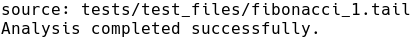
\includegraphics[width=0.7\textwidth]{imagenes/fib1.png}
		\caption{Resultado del análisis de la sucesión de Fibonacci.}
		\label{fig:fib1}
	\end{center}
\end{figure}

Ahora le realizaremos un pequeño cambio al código. En vez de llamar a la función \textit{fib} con el parámetro $3$, lo haremos con \textit{True}. El código se encuentra en \textit{tests/test\_files/fibonacci\_2.tail}.\\

\begin{lstlisting}[style=tail]
fib : Int -> Int
fib(n) :=
	if n <= 1 then
		1
	else
		fib(n-1) + fib(n-2)

write("fib(True) = {fib(True)}")
\end{lstlisting}

El sistema de tipos debería detectar que \textit{True} no es de tipo \textit{Int} y comunicárnoslo, y eso es lo que ocurre. El resultado se puede ver en la figura \ref{fig:fib2}\\

\begin{figure}[H]
	\begin{center}
		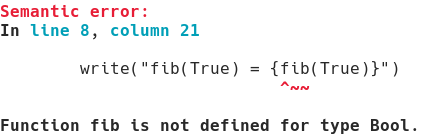
\includegraphics[width=0.7\textwidth]{imagenes/fib2.png}
		\caption{Resultado del análisis de la sucesión de Fibonacci con un parámetro incorrecto.}
		\label{fig:fib2}
	\end{center}
\end{figure}

Cambiaremos de nuevo este código para mostrar como también se detecta cuando una variable no ha sido declarada. Este código se puede encontrar en \textit{tests/test\_files/fibonacci\_3.tail}.\\

\begin{lstlisting}[style=tail]
fib : Int -> Int
fib(n) :=
	if x <= 1 then
		1
	else
		fib(n-1) + fib(n-2)

write("fib(3) = {fib(3)}")
\end{lstlisting}

Se puede ver como se captura el error en la figura \ref{fig:fib3}.\\

\begin{figure}[H]
	\begin{center}
		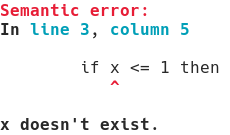
\includegraphics[width=0.35\textwidth]{imagenes/fib3.png}
		\caption{Resultado del análisis de la sucesión de Fibonacci con una variable inexistente.}
		\label{fig:fib3}
	\end{center}
\end{figure}

Modificaremos este código una última vez para ver que ocurre cuando usamos una variable que se nos ha olvidado inicializar. Se puede encontrar este código en \textit{tests/test\_files/fibonacci\_4.tail}.\\

\begin{lstlisting}[style=tail]
fib : Int -> Int
fib(n) :=
	if n <= 1 then
		1
	else
		fib(n-1) + fib(n-2)

x : Int

write("fib(x) = {fib(x)}")
\end{lstlisting}

Como se ve en la figura \ref{fig:fib4} el analizador semántico se da cuenta del fallo.\\

\begin{figure}[H]
	\begin{center}
		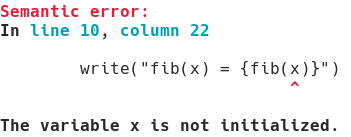
\includegraphics[width=0.55\textwidth]{imagenes/fib4.png}
		\caption{Resultado del análisis de la sucesión de Fibonacci con una variable sin inicializar.}
		\label{fig:fib4}
	\end{center}
\end{figure}

Veamos ahora dos programas que utilizan la unión de tipos. Mientras que el primero es completamente correcto, en el segundo a la variable $x$ se le asigna un valor de un tipo diferente al que se le ha declarado. El código se encuentra en \textit{tests/test\_files/union\_types\_1.tail} y \textit{tests/test\_files/union\_types\_2.tail} respectivamente.\\

\begin{lstlisting}[style=tail]
f : Bool -> :Hola or String

f(b) := if b then :hola else "hola"

x : Atom or String
x := f(True)

write("f(true) = {x}")
\end{lstlisting}

\begin{lstlisting}[style=tail]
f : Bool -> :Hola or String

f(b) := if b then :hola else "hola"

x : Atom or Int
x := f(True)

write("f(true) = {x}")
\end{lstlisting}

El análisis del primer programa termina correctamente, como se muestra en la figura \ref{fig:un1}.

\begin{figure}[H]
	\begin{center}
		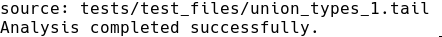
\includegraphics[width=0.7\textwidth]{imagenes/union1.png}
		\caption{Resultado del análisis de la unión de tipos.}
		\label{fig:un1}
	\end{center}
\end{figure}

En el segundo, en cambio, se detecta el error y se muestra por pantalla, siendo visible en la figura \ref{fig:un2}.\\

\begin{figure}[H]
	\begin{center}
		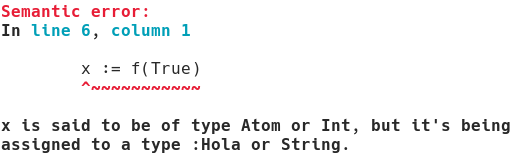
\includegraphics[width=0.75\textwidth]{imagenes/union2.png}
		\caption{Resultado del análisis de una asignación incorrecta con unión de tipos.}
		\label{fig:un2}
	\end{center}
\end{figure}


Hacemos ahora lo análogo con la intersección de tipos. A continuación se muestran dos programas, uno correcto y otro con una asignación del tipo equivocado. El código se encuentra en \textit{tests/test\_files/intersection\_types\_1.tail} y \textit{tests/test\_files/intersection\_types\_2.tail}. En las figuras \ref{fig:in1} y \ref{fig:in2} se muestra la salida de la ejecución.\\

\begin{lstlisting}[style=tail]
x : (:A1 or :A2) and (:A2 or :A3)
x := :a2

write("x = {x}")
\end{lstlisting}

\begin{figure}[H]
	\begin{center}
		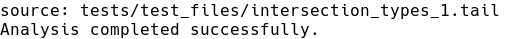
\includegraphics[width=0.75\textwidth]{imagenes/int1.png}
		\caption{Resultado del análisis de la intersección de tipos.}
		\label{fig:in1}
	\end{center}
\end{figure}

\begin{lstlisting}[style=tail]
x : (:A1 or :A2) and (:A2 or :A3)
x := :a3

write("x = {x}")
\end{lstlisting}

\begin{figure}[H]
	\begin{center}
		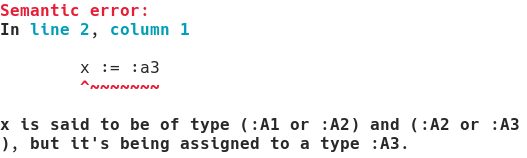
\includegraphics[width=0.75\textwidth]{imagenes/int2.png}
		\caption{Resultado del análisis de la intersección de tipos con una asignación incorrecta.}
		\label{fig:in2}
	\end{center}
\end{figure}


Para terminar comprobamos que el análisis de los tipos graduales funciona correctamente. En este primer fragmento de código, disponible en \textit{tests/test\_files/gradual\_types\_1.tail}, se ve como es posible pasar como argumento valores de diferentes tipos. En la figura \ref{fig:grad1} se muestra que el análisis termina correctamente.\\

\begin{lstlisting}[style=tail]
f : ?, Bool -> ? or String
f(x, b) := if b then x else "Nada"

write("f(3, True) = {f(3, True)}")
write("f(:hola, True) = {f(:hola, True)}")
\end{lstlisting}

\begin{figure}[H]
	\begin{center}
		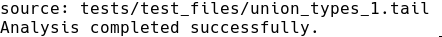
\includegraphics[width=0.7\textwidth]{imagenes/grad1.png}
		\caption{Resultado del análisis de tipos graduales.}
		\label{fig:grad1}
	\end{center}
\end{figure}

En cambio, cuando usamos un argumento del tipo incorrecto en el segundo parámetro, como en el siguiente código, el analizador lo detecta, como se muestra en la figura \ref{fig:grad2}. El código se puede encontrar en \textit{tests/test\_files/gradual\_types\_2.tail}.\\

\begin{lstlisting}[style=tail]
f : ?, Bool -> ? or String
f(x, b) := if b then x else "Nada"

write("f(3, :no_bool) = {f(3, :no_bool)}")
\end{lstlisting}

\begin{figure}[H]
	\begin{center}
		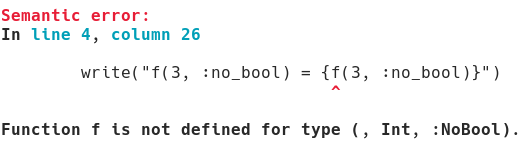
\includegraphics[width=0.8\textwidth]{imagenes/grad2.png}
		\caption{Resultado del análisis de tipos graduales con un argumento incorrecto.}
		\label{fig:grad2}
	\end{center}
\end{figure}

Así, damos por concluida la presentación de diferentes ejecuciones y con ello el capítulo dedicado a la implementación.\\
%
\chapter{Conclusiones y trabajo futuro}
\label{sect:con}

En este trabajo hemos abordado elementos fundamentales de la teoría de lenguajes de programación. Hemos visto como se relaciona la teoría de tipos matemática con su aplicación en lenguajes, mediante el estudio de los sistemas de tipado y su capacidad para codificar el funcionamiento de sistemas tipos que comprueban el buen uso de los tipos teóricos.\\

También se han presentado técnicas fundamentales como la demostración de la seguridad de un lenguaje mediante los teoremas de progreso y preservación y la comprobación de la turing-completitud haciendo uso de las funciones $\mu$-recursivas.\\

Se ha demostrado que el análisis de un lenguaje es una fase fundamental en su diseño y que los trabajos realizados en este campo dan como resultado mejoras tangibles en la calidad de los lenguajes que utilizamos diariamente. Sin embargo, aún queda mucho espacio para profundizar en los aspectos teóricos. Una vía de investigación futura interesante sería el estudio de la teoría de tipos dependientes, tanto sus posibles aplicaciones como sus implicaciones teóricas y sus conexiones con la lógica mediante el isomorfismo de Curry-Howard.\\

Respecto a la parte práctica, hemos diseñado un nuevo lenguaje, identificando los factores que lo pueden hace útil al usarlo en inteligencia artificial. Se ha formalizando su sintaxis, semántica y sistema de tipos y se han aplicado los resultados teóricos aprendidos para demostrar su buen comportamiento. A su vez se ha realizado una implementación parcial de su compilador, aprendiendo por el camino que antes de invertir tiempo en una tecnología es necesario cerciorarse de que se adecúa a nuestras necesidades. Una línea de trabajo evidente sería la conclusión del compilador, eligiendo un método de generación de código más adecuado. Otros elementos interesantes para desarrollar sería el diseño de un sistema de módulos para \textit{tail} y la adición de facilidades para la programación concurrente.\\
%\input{capitulos/07_Pruebas}
%
%\input{capitulos/08_Conclusiones}
%
%%\chapter{Conclusiones y Trabajos Futuros}
%
%
\nocite{*}
\bibliography{bibliografia}\addcontentsline{toc}{chapter}{Bibliografía}
\bibliographystyle{plain}
%\bibliographystyle{miunsrturl}
%
\begin{appendices}
\renewcommand{\thesection}{\Alph{section}}
\section{Sintaxis de tail.}
\label{apendice:sintaxis_tail}

\begin{grammar}{t}{términos}
(t)           & paréntesis \\
t;t           & secuencia \\
x             & variable \\
x := t        & asignación \\
x : \tau      & declaración tipo \\
\ \<typeof> t   & operador typeof \\
n             & constante numérica \\
-t            & operador opuesto \\
t + t         & operador suma \\
t - t         & operador resta \\
t * t         & operador producto \\
t / t         & operador cociente \\
t // t        & operador fracción \\
t \% t        & operador módulo \\
t\ \hat{}\ t & operador exponenciación \\
\ \<match>\ t\ \<with>\ n\ \mathligsoff -> \mathligson\ t & match numérico \\
\ \<match>\ t\ \<with>\ \_\ \mathligsoff -> \mathligson\ t & match por defecto \\
``t^s"         & constante string \\
\ :x            & átomo \\
True          & constante true \\
False          & constante false \\
t \<and> t        & operador and \\
t \<or> t         & operador or \\
t \<xor> t        & operador xor \\
\ \<not> t          & operador not \\
t = t          & operador igualdad \\
t != t         & operador desigualdad \\
t < t          & operador menor \\
t \mathligsoff <= \mathligson t         & operador menor-igual \\
t > t          & operador mayor \\
t >= t         & operador mayor-igual \\
\ \<if> t \<then> t\ \{\<elif> t \<then> t\} \<else> t & condicional \\
\ \<lambda> x.t     & función lambda \\
t(t)          & aplicación \\
t.t(t)        & método \\
... \\
\end{grammar}

\hspace*{-2cm}
\begin{grammar}{t}{términos}
... \\
t_i^{i \in 1...n} & tupla \\
\ \<match>\ t\ \<with>\ t_i^{i \in 1...n} \mathligsoff -> \mathligson\ t & match tupla \\
\ <t_i^{i \in 1...n}> & lista \\
\ \<match>\ t\ \<with>\ <x \mid \overline{x}> \mathligsoff -> \mathligson\ t & match lista \\
{} [{t_i}^{i \in 1...n}] & vector \\
{} [t_{ij}^{\stackrel{i \in 1...n}{j \in 1...m}}] & matriz \\
{t_i => \overline{t}_i}^{i \in 1...n} & diccionario\\
t[t]          & operador proyección \\
\ \<variant> V::C_i({l_{ij} : \tau_{ij}}^{j \in 1...r_i})^{i \in 1...n} & declaración variant \\
V::C_i(t_{ij})^{j \in 1...r_i} & instancia variant \\
t.t           & acceso atributo \\
\ \<match> t \<with> V::C_i(t_{ij})^{j \in 1...r_i} \mathligsoff -> \mathligson\ t & match variant \\
\end{grammar}

\bigskip
\hspace*{-2cm}
\begin{grammar}{v}{valores}
n             & constante numérica \\
True          & constante true \\
False          & constante false \\
``t^s"         & constante string \\
\ :x            & átomo \\
\ \<lambda> x.t     & función lambda \\
t_i^{i \in 1...n} & tupla \\
\ <t_i^{i \in 1...n}> & lista \\
{} [{t_i}^{i \in 1...n}] & vector \\
{} [t_{ij}^{\stackrel{i \in 1...n}{j \in 1...m}}] & matriz \\
{t_i => \overline{t}_i}^{i \in 1...n} & diccionario\\
V::C_i(t_{ij})^{j \in 1...r_i} & instancia variant \\
\end{grammar}

\bigskip
\hspace*{-2cm}
\begin{grammar}{T}{tipos estáticos}
B                            & tipos base \\ % Int, String, :<NombreAtomo>, ...
T -> T                       & tipo función \\
T \<or> T                    & unión de tipos \\
T \<and> T                   & intersección de tipos \\
\ \<not> T                     & negación de tipos \\
Void                         & tipo vacío \\
U                            & tipo universal \\
{T_i}^{i \in 1...n}          & tipo tupla \\
List \<of> T                 & tipo lista \\
Vector \<of> T               & tipo vector \\
Dictionary \<of> T, T        & tipo diccionario \\
Matrix \<of> T               & tipo matriz \\
\end{grammar}

\bigskip
\begin{grammar}{\tau}{tipos graduales}
\ ?                            & tipo desconocido \\
B                            & tipos base \\ % Int, String, :<NombreAtomo>, ...
\tau -> \tau                 & tipo función \\
\tau \<or> \tau              & unión de tipos \\
\tau \<and> \tau             & intersección de tipos \\
\ \<not> T                     & negación de tipos \\
Void                         & tipo vacío \\
U                            & tipo universal \\
{\tau_i}^{i \in 1...n}       & tipo tupla \\
List\ [\<of> \tau]           & tipo lista \\
Vector\ [\<of> \tau]         & tipo vector \\
Dictionary\ [\<of> \tau, \tau]      & tipo diccionario \\
Matrix\ [\<of> \tau]         & tipo matriz \\
\end{grammar}

\bigskip
\begin{grammar}{\Gamma}{contexto}
\o               & contexto vacío \\
\Gamma, x:\tau   & anotación de tipo \\
\Gamma, x:=t     & asignación de valor \\
\end{grammar}

\newpage
\section{Reglas de evaluación de tail.}
\label{apendice:evaluacion_tail}

\begin{figure}[p]
\caption{Reglas de evaluación de tail.}
\label{fig:evtail}

\bigskip
\bigskip

\inference[E-AssigRed:]{t -> t'}{x \<:=> t -> x \<:=> t'}

\bigskip

\inference[E-Assig:]
{x \<:=> v}
{\begin{array}{@{}c@{}}
\Gamma |- x \<:=> v \\
x\<:=>v -> v
\end{array}}

\bigskip

\inference[E-Var:]{\Gamma |- x \<:=> v}{x -> v}

\bigskip

\inference[E-TypeDec:]{}{t:\tau -> t}

\bigskip

\inference[E-Typeof:]{\Gamma |- t : \tau}{\<typeof> t -> string(\tau)}

\bigskip

\inference[E-FuncSintSug:]{}{f(x) := t -> f := \<lambda> x.t}

\bigskip

\inference[E-App:]{}{\<lambda> x . t (v) -> [x |-> v]t}

\bigskip

\inference[E-AppParameterRed:]{t -> t'}{\<lambda> x . \overline{t} (t) -> \<lambda> x . \overline{t} (t')}

\bigskip

\inference[E-AppRed:]{t_1 -> t_1'}{t_1(t_2) -> t_1'(t_2)}

\bigskip

\inference[E-If:]{}{\<if> True \<then> t_1 \<else> t_2 -> t_1}

\bigskip

\inference[E-Else:]{}{\<if> False \<then> t_1 \<else> t_2 -> t_2}

\bigskip

\inference[E-IfRed:]{t_1 -> t_1'}{\<if> t_1 \<then> t_2 \<else> t_3 -> \<if> t_1' \<then> t_2\ \<else> t_3}

\bigskip

\inference[E-Seq:]{t_1 -> t_1'}{t_1 \<;> t_2 -> t_1' \<;> t_2}

\bigskip

\inference[E-SeqNext:]{}{v \<;> t -> t}

\bigskip

\inference[E-ParRed:]{t -> t'}{(t) -> (t')}

\bigskip

\inference[E-Par:]{}{(v) -> v}

\bigskip

\inference[E-BlockRed:]
{t -> t'}
{
\Gamma' := \Gamma, \\
BeginBlock\ t\ EndBlock ->_{\Gamma'} BeginBlock\ t'\ EndBlock
}

\bigskip

\inference[E-Block:]{}{BeginBlock\ v\ EndBlock -> v}

\end{figure}


\begin{figure}[p]

\bigskip
\bigskip

\inference[E-String:]{}{``v^s \{v\} t^s" -> ``v^s" + string(v) + ``t^s"}

\bigskip

\inference[E-StringRed:]{t -> t'}{``v^s \{t\} t^s" -> ``v^s \{t'\} t^s"}

\inference[E-SubTypeTrue:]{\tau_1 ~< \tau_2}{\tau_1 \<<:> \tau_2 -> True}

\bigskip

\inference[E-SubTypeFalse:]{\tau_1 \ \widetilde{\nleq}\ \tau_2}{\tau_1 \<<:> \tau_2 -> False}

\bigskip

\inference[E-VariantDec:]{}{
\begin{array}{@{}c@{}}
\<variant> V \<::> C_1(l_{1 1} : \tau_{11}, ..., l_{1r_1} : \tau_{1r_1}) \mid ... \mid C_n(l_{n 1} : \tau_{n 1}, ..., l_{nr_n} : \tau_{nr_n}) -> \\
-> <{V::C_i(l_{ij} : \tau_{ij}}^{j \in 1...r_i})^{i \in 1...n}> \\
\Gamma |- V := {V::C_i({l_{ij} : \tau_{ij}}^{j \in 1...r_i})}^{i \in 1...n}
\end{array}}

\bigskip

\inference[E-VariantConstruct:]{\Gamma |- V := {V::C_i(l_{ij} : \tau_{ij}}^{j \in 1...r_i})^{i \in 1...n}}{
\begin{array}{@{}c@{}}
\Gamma |- V::C_i := \lambda x_1, ..., x_{r_i}.V::C_i(l_{ij} : \tau_{ij}^{j \in 1 ... r_i})^{i \in 1...n}
\end{array}}

\bigskip

\inference[E-ProjectionVariant:]{
\<variant> {V::C_i(x_{ij} : \tau_{ij}}^{j \in 1...r_i})^{i \in 1...n} \in \Gamma
}{
V::C_i(t_{i1}, ..., t_{in}).x_{ik} -> t_{ik}
}

\bigskip

\inference[E-DotRed:]{t_1 -> t'_1}{t_1.x -> t'_1.x}

\bigskip

\inference[E-MethodSintSug:]{}{t_1.t_2(t_3) -> t_2(t_1, t_3)}

\bigskip

\inference[E-MatchRed:]{t_0 -> t'_0}{
\begin{array}{@{}c@{}}
\<match> t_0 \<with>\ t_{1i}\ \mathligsoff -> \mathligson\ t_{2i} -> \\
->\ \<match> t'_0 \<with>\ t_{1i}\ \mathligsoff -> \mathligson\ t_{2i}
\end{array}}

\bigskip

\inference[E-MatchPatternRed:]{t_{1i} -> t'_{1i}}{
\begin{array}{@{}c@{}}
\<match> v \<with>\ t_{1i}\ \mathligsoff -> \mathligson\ t_{2i} -> \\
->\ \<match> v \<with>\ t'_{1i}\ \mathligsoff -> \mathligson\ t_{2i}
\end{array}}

\bigskip

\inference[E-MatchEqual:]{v_i=v_0\ y\ v_j \neq v_0\ \forall\ 0 < j < i}{
\begin{array}{@{}c@{}}
\<match>\ v_0 \<with> v_i\ \mathligsoff -> \mathligson\ t_i -> t_i
\end{array}}

\bigskip

\inference[E-MatchAny:]{}{
\begin{array}{@{}c@{}}
\<match>\ v \<with> \_\ \mathligsoff -> \mathligson\ t_i -> t_i
\end{array}}

\bigskip

\inference[E-MatchVariant:]{}{
\begin{array}{@{}c@{}}
\<match>\ V::C_i(v_1, ..., v_n) \<with>\\
V::C_i(x_1, ..., x_n)\ \mathligsoff -> \mathligson\ t_i -> [x_i |-> v_i]t_i
\end{array}}

\bigskip

\end{figure}


\begin{figure}[p]

\bigskip
\bigskip

\inference[E-Tuple:]
{t_j -> t'_j}
{v_i^{i \in 1...j-1}, t_j, t_k^{k \in j+1...n} -> v_i^{i \in 1...j-1}, t'_j, t_k^{k \in j+1...n}}

\bigskip

\inference[E-AssigTuple:]
{}
{x_i^{i \in 1...n} := t_i^{i \in 1...n} -> x_i := t_i\ i \in 1...n}

\bigskip

\inference[E-MatchTuple:]{}
{\<match>\ v_i^{i \in 1...n} \<with>\ x_i^{i \in 1...n} \mathligsoff -> \mathligson\ t ->
[x_i |-> v_i]t}

\bigskip


\inference[E-List:]
{t_j -> t'_j}
{<v_i^{i \in 1...j-1}\ t_j\ t_k^{k \in j+1...n}> -> <v_i^{i \in 1...j-1}\ t'_j\ t_k^{k \in j+1...n}>}

\bigskip

\inference[E-MatchList:]{}
{\<match>\ <v_i^{i \in 1...n}>\ \<with>\ <x \mid \overline{x}> \mathligsoff -> \mathligson\ t ->
[x |-> v_1, \overline{x} |-> <v_i^{i \in 2...n}>]t}

\bigskip

\inference[E-Vector:]
{t_j -> t'_j}
{[v_i^{i \in 1...j-1}\ t_j\ t_k^{k \in j+1...n}] -> [v_i^{i \in 1...j-1}\ t'_j\ t_k^{k \in j+1...n}]}

\bigskip

\inference[E-Matrix:]
{t_{rk} -> t'_{rk}}
{[v_{ij}^{\stackrel{i \in 1...r-1}{j \in 1...m}} \mid
v_{rj}^{j \in 1...k-1}\ t_{rk}\ t_{rj}^{j \in k+1...m} \mid
v_{ij}^{\stackrel{i \in r+1...n}{j \in 1...m}}] ->
[v_{ij}^{\stackrel{i \in 1...r-1}{j \in 1...m}} \mid
v_{rj}^{j \in 1...k-1}\ t'_{rk}\ t_{rj}^{j \in k+1...m} \mid
v_{ij}^{\stackrel{i \in r+1...n}{j \in 1...m}}]}

\bigskip

\inference[E-DictKey:]
{t_j -> t'_j}
{{v_i => \overline{v}_i}^{i \in 1...j-1}, t_j => \overline{t}_j, {t_k => \overline{t}_k}^{k \in j+1...n} -> 
{v_i => \overline{v}_i}^{i \in 1...j-1}, t'_j => \overline{t}_j, {t_k => \overline{t}_k}^{k \in j+1...n}}

\bigskip

\inference[E-DictValue:]
{\overline{t}_j -> \overline{t'}_j}
{{v_i => \overline{v}_i}^{i \in 1...j-1}, v_j => \overline{t}_j, {t_k => \overline{t}_k}^{k \in j+1...n} -> 
{v_i => \overline{v}_i}^{i \in 1...j-1}, v_j => \overline{t'}_j, {t_k => \overline{t}_k}^{k \in j+1...n}}
\end{figure}

\newpage
\section{Reglas de tipado de tail.}
\label{apendice:tipos_tail}

\begin{figure}[p]
\caption{Reglas de tipado de tail.}
\label{fig:tiptail}

\bigskip
\bigskip

\inference[T-Basic:]{}{\Gamma |- c:B(c)}

\bigskip

\inference[T-TypeDec:]{t:\tau \in \Gamma}{
\begin{array}{@{}c@{}}
\Gamma |- t : \tau\\
\Gamma |- (t:\tau) : \tau
\end{array}}

\bigskip

\inference[T-Assig:]{\Gamma |- t:\tau_1, \Gamma |- x:\tau_2, \tau_1 ~< \tau_2\ \acute{o}\ \tau_2 = ?}{\Gamma |- x \<:=> t : \tau_2}

\bigskip

\inference[T-Typeof:]{\Gamma |- t:\tau}{\Gamma |- \<typeof> t : String}

\bigskip

\inference[T-App:]
{\Gamma |- f:\tau_1, \Gamma |- t:\tau_2, \tau_1 ~< \mathbb{0} -> \mathbb{1}, \tau_2 ~< \widetilde{dom}(\tau_1)}
{\Gamma |- f(t) : \tau_1 \widetilde{\circ} \tau_2}

\bigskip

\inference[T-Lambda:]
{\Gamma, x:\tau_1 |- \overline{t}:\tau_2}
{\Gamma |- \<lambda> x.\overline{t} : \tau_1 -> \tau_2}

\bigskip

\inference[T-If:]
{\Gamma |- t_1 : Bool, \Gamma |- t_2:\tau_2, \Gamma |- t_3:\tau_3}
{\Gamma |- \<if> t_1 \<then> t_2 \<else> t_3 : \tau_2 \vee \tau_3}

\bigskip

\inference[T-Seq:]
{\Gamma |- t1:\tau_1, \Gamma |- t2:\tau_2}
{\Gamma |- t1\<;>t2 : \tau_2}

\bigskip

\inference[T-Par:]{\Gamma |- t:\tau}{\Gamma |- (t):\tau}

\bigskip

\inference[T-Block:]{\Gamma |- t:\tau}{\Gamma |- BeginBlock\ t\ EndBlock : \tau}

\bigskip

\inference[T-VariantConstructor:]{\<variant> V::C_i({x_{ij} : \tau_{ij}}^{j \in 1...r_i})^{i \in 1...n} \in \Gamma}
{\Gamma |- V::C_i(t_{i1}, ..., t_{in}) : V}

\bigskip

\inference[T-ProjectionVariant:]{\<variant> {V::C_i(x_{ij} : \tau_{ij}}^{j \in 1...r_i})^{i \in 1...n} \in \Gamma \\
\Gamma |- t_{ij} : \tau_{ij}\ \ j \in 1...r_i}
{\Gamma |- V::C_i(t_{i1}, ..., t_{in}).x_{ik} : \tau_{ik}}

\bigskip

\inference[T-Match:]{
\Gamma |- t_0 : \tau\ t.q\ \exists\ \cdot=\cdot\ : \tau_e \in \Gamma\ con\ \tau_e ~< \mathbb{0} -> U,\ \tau ~< \widetilde{dom}(\tau_e)\ y\ \tau_e \widetilde{\circ} \tau = Bool\\
\Gamma |- t_{1i}:\tau,\ \Gamma |- t_{2i} : \tau_i}
{\Gamma |- \<match> t_0 \<with>\ t_{1i} \mathligsoff -> \mathligson\ t_{2i} : \bigvee_{i=1}^n \tau_i}

\bigskip

\inference[T-MatchVariant:]{
\<variant> V::C_i({x_{ij} : \tau_{ij}}^{j \in 1...r_i})^{i \in 1...n} \in \Gamma \\
\Gamma |- t_0 : V\ \ \Gamma, x_{ij}:\tau_{ij} |- t_i : \tau_i}
{\Gamma |- \<match> t_0 \<with>\ V::C_i(x_{i1}, ..., x_{ir_i})\ \mathligsoff -> \mathligson\ t_i : \bigvee_{i=1}^m \tau_i}

\end{figure}


\begin{figure}[p]

\bigskip
\bigskip

\inference[T-Tuple:]
{\Gamma |- t_i : \tau_i\ i \in 1...n}
{\Gamma |- {t_i}^{i \in 1...n} : {\tau_i}^{i \in 1...n}}


\bigskip

\inference[T-MatchTuple:]{
\Gamma |- t_0 : {\tau_{0i}} ^ {i \in 1...n}\ \
\Gamma, x_i:\tau_{0i} |- t_{2i} : \tau_i}
{\Gamma |- \<match> t_0 \<with>\ x_1, ..., x_m\ \mathligsoff -> \mathligson\ t_{2i} : \bigvee_{i=1}^m \tau_i}


\bigskip

\inference[T-List:]
{\Gamma |- t_i : \tau\ i \in 1...n}
{\Gamma |- <{t_i}^{i \in 1...n}> : List \<of> \tau}


\bigskip

\inference[T-MatchList:]{
\Gamma |- t_0 : List \<of> \tau \\
\Gamma, x_i:\tau, \overline{x}_i : List \<of> \tau |- t_i : \tau_i}
{\Gamma |- \<match> t_0 \<with>\ <x_i \mid \overline{x}_i>\ \mathligsoff -> \mathligson\ t_i : \bigvee_{i=1}^n \tau_i}

\bigskip

\inference[T-Vector:]
{\Gamma |- t_i : \tau\ i \in 1...n}
{\Gamma |- [{t_i}^{i \in 1...n}] : Vector \<of> \tau}

\bigskip

\inference[T-Matrix:]
{\Gamma |- t_i : \tau\ i \in 1...n,\ j \in 1...m}
{\Gamma |- [{t_{ij}}^{\stackrel{i \in 1...n}{j \in 1...m}}] : Matrix \<of> \tau}

\bigskip

\inference[T-Dictionary:]
{\Gamma |- t_i : \tau,\ \Gamma |- \overline{t}_i : \overline{\tau}\ i \in 1...n}
{\Gamma |- {t_i => \overline{t}_i}^{i \in 1...n} : Dictionary \<of> \tau, \overline{\tau}}

\end{figure}

\end{appendices}

%\input{glosario/entradas_glosario}
% \addcontentsline{toc}{chapter}{Glosario}
% \printglossary
\chapter*{}
\thispagestyle{empty}

\end{document}
